% ******************************* PhD Thesis Template **************************
% Please have a look at the README.md file for info on how to use the template

\documentclass[a4paper,12pt,customfont,numbered,index]{Classes/PhDThesisPSnPDF}

% ******************************************************************************
% ******************************* Class Options ********************************
% *********************** See README for more details **************************
% ******************************************************************************

% `a4paper'(The University of Cambridge PhD thesis guidelines recommends a page
% size a4 - default option) or `a5paper': A5 Paper size is also allowed as per
% the Cambridge University Engineering Deparment guidelines for PhD thesis
%
% `11pt' or `12pt'(default): Font Size 10pt is NOT recommended by the University
% guidelines
%
% `oneside' or `twoside'(default): Printing double side (twoside) or single
% side.
%
% `print': Use `print' for print version with appropriate margins and page
% layout. Leaving the options field blank will activate Online version.
%
% `index': For index at the end of the thesis
%
% `draftclassic': For draft mode without loading any images (same as draft in book)
%
% `draft': Special draft mode with line numbers, images, and water mark with
% timestamp and custom text. Position of the text can also be modified.
%
% `abstract': To generate only the title page and abstract page with
% dissertation title and name, to submit to the Student Registry
%
% `chapter`: This option enables only the specified chapter and it's references
%  Useful for review and corrections.
%
% ************************* Custom Page Margins ********************************
%
% `custommargin`: Use `custommargin' in options to activate custom page margins,
% which can be defined in the preamble.tex. Custom margin will override
% print/online margin setup.
%
% *********************** Choosing the Fonts in Class Options ******************
%
% `times' : Times font with math support. (The Cambridge University guidelines
% recommend using times)
%
% `fourier': Utopia Font with Fourier Math font (Font has to be installed)
%            It's a free font.
%
% `customfont': Use `customfont' option in the document class and load the
% package in the preamble.tex
%
% default or leave empty: `Latin Modern' font will be loaded.
%
% ********************** Choosing the Bibliography style ***********************
%
% `authoryear': For author-year citation eg., Krishna (2013)
%
% `numbered': (Default Option) For numbered and sorted citation e.g., [1,5,2]
%
% `custombib': Define your own bibliography style in the `preamble.tex' file.
%              `\RequirePackage[square, sort, numbers, authoryear]{natbib}'.
%              This can be also used to load biblatex instead of natbib
%              (See Preamble)
%
% **************************** Choosing the Page Style *************************
%
% `default (leave empty)': For Page Numbers in Header (Left Even, Right Odd) and
% Chapter Name in Header (Right Even) and Section Name (Left Odd). Blank Footer.
%
% `PageStyleI': Chapter Name next & Page Number on Even Side (Left Even).
% Section Name & Page Number in Header on Odd Side (Right Odd). Footer is empty.
%
% `PageStyleII': Chapter Name on Even Side (Left Even) in Header. Section Number
% and Section Name in Header on Odd Side (Right Odd). Page numbering in footer

% Uncomment to change page style
%\pagestyle{PageStyleII}

% ********************************** Preamble **********************************
% Preamble: Contains packages and user-defined commands and settings
% ******************************************************************************
% ****************************** Custom Margin *********************************

% Add `custommargin' in the document class options to use this section
% Set {innerside margin / outerside margin / topmargin / bottom margin}  and
% other page dimensions
\ifsetCustomMargin
  \RequirePackage[left=37mm,right=30mm,top=35mm,bottom=30mm]{geometry}
  \setFancyHdr % To apply fancy header after geometry package is loaded
\fi

% Add spaces between paragraphs
%\setlength{\parskip}{0.5em}
% Ragged bottom avoids extra whitespaces between paragraphs
\raggedbottom
% To remove the excess top spacing for enumeration, list and description
%\usepackage{enumitem}
%\setlist[enumerate,itemize,description]{topsep=0em}

% *****************************************************************************
% ******************* Fonts (like different typewriter fonts etc.)*************

% Add `customfont' in the document class option to use this section

\ifsetCustomFont
  % Set your custom font here and use `customfont' in options. Leave empty to
  % load computer modern font (default LaTeX font).
  %\RequirePackage{helvet}
  \RequirePackage{lmodern}

  % For use with XeLaTeX
  %  \setmainfont[
  %    Path              = ./libertine/opentype/,
  %    Extension         = .otf,
  %    UprightFont = LinLibertine_R,
  %    BoldFont = LinLibertine_RZ, % Linux Libertine O Regular Semibold
  %    ItalicFont = LinLibertine_RI,
  %    BoldItalicFont = LinLibertine_RZI, % Linux Libertine O Regular Semibold Italic
  %  ]
  %  {libertine}
  %  % load font from system font
  %  \newfontfamily\libertinesystemfont{Linux Libertine O}
\fi

% *****************************************************************************
% **************************** Custom Packages ********************************

% ************************* Algorithms and Pseudocode **************************

%\usepackage{algpseudocode}


% ********************Captions and Hyperreferencing / URL **********************

% Captions: This makes captions of figures use a boldfaced small font.
%\RequirePackage[small,bf]{caption}

\RequirePackage[labelsep=space,tableposition=top]{caption}
\renewcommand{\figurename}{Fig.} %to support older versions of captions.sty


% *************************** Graphics and figures *****************************

%\usepackage{rotating}
%\usepackage{wrapfig}

% Uncomment the following two lines to force Latex to place the figure.
% Use [H] when including graphics. Note 'H' instead of 'h'
%\usepackage{float}
%\restylefloat{figure}

% Subcaption package is also available in the sty folder you can use that by
% uncommenting the following line
% This is for people stuck with older versions of texlive
%\usepackage{sty/caption/subcaption}
\usepackage{subcaption}

% ********************************** Tables ************************************
\usepackage{booktabs} % For professional looking tables
\usepackage{multirow}

%\usepackage{multicol}
%\usepackage{longtable}
%\usepackage{tabularx}


% *********************************** SI Units *********************************
\usepackage{siunitx} % use this package module for SI units
\sisetup{
detect-weight = true,
detect-inline-weight = math
}

% ******************************* Line Spacing *********************************

% Choose linespacing as appropriate. Default is one-half line spacing as per the
% University guidelines

% \doublespacing
% \onehalfspacing
% \singlespacing


% ************************ Formatting / Footnote *******************************

% Don't break enumeration (etc.) across pages in an ugly manner (default 10000)
%\clubpenalty=500
%\widowpenalty=500

%\usepackage[perpage]{footmisc} %Range of footnote options


% *****************************************************************************
% *************************** Bibliography  and References ********************

\usepackage{cleveref} %Referencing without need to explicitly state fig /table

% Add `custombib' in the document class option to use this section
\ifuseCustomBib
   \RequirePackage[square, sort, numbers, authoryear]{natbib} % CustomBib

% If you would like to use biblatex for your reference management, as opposed to the default `natbibpackage` pass the option `custombib` in the document class. Comment out the previous line to make sure you don't load the natbib package. Uncomment the following lines and specify the location of references.bib file

%\RequirePackage[backend=biber, style=numeric-comp, citestyle=numeric, sorting=nty, natbib=true]{biblatex}
%\bibliography{References/references} %Location of references.bib only for biblatex

\fi

% changes the default name `Bibliography` -> `References'; also rewritten in the thesis.tex
\renewcommand{\bibname}{References}


% ******************************************************************************
% ************************* User Defined Commands ******************************
% ******************************************************************************

% *********** To change the name of Table of Contents / LOF and LOT ************

%\renewcommand{\contentsname}{My Table of Contents}
%\renewcommand{\listfigurename}{My List of Figures}
%\renewcommand{\listtablename}{My List of Tables}


% ********************** TOC depth and numbering depth *************************

\setcounter{secnumdepth}{2}
\setcounter{tocdepth}{2}


% ******************************* Nomenclature *********************************

% To change the name of the Nomenclature section, uncomment the following line

%\renewcommand{\nomname}{Symbols}


% ********************************* Appendix ***********************************

% The default value of both \appendixtocname and \appendixpagename is `Appendices'. These names can all be changed via:

%\renewcommand{\appendixtocname}{List of appendices}
%\renewcommand{\appendixname}{Appndx}

% *********************** Configure Draft Mode **********************************

% Uncomment to disable figures in `draft'
%\setkeys{Gin}{draft=true}  % set draft to false to enable figures in `draft'

% These options are active only during the draft mode
% Default text is "Draft"
%\SetDraftText{DRAFT}

% Default Watermark location is top. Location (top/bottom)
%\SetDraftWMPosition{bottom}

% Draft Version - default is v1.0
%\SetDraftVersion{v1.1}

% Draft Text grayscale value (should be between 0-black and 1-white)
% Default value is 0.75
%\SetDraftGrayScale{0.8}


% ******************************** Todo Notes **********************************
%% Uncomment the following lines to have todonotes.

%\ifsetDraft
%	\usepackage[colorinlistoftodos]{todonotes}
%	\newcommand{\mynote}[1]{\todo[author=kks32,size=\small,inline,color=green!40]{#1}}
%\else
%	\newcommand{\mynote}[1]{}
%	\newcommand{\listoftodos}{}
%\fi

% Example todo: \mynote{Hey! I have a note}


% ************************ Thesis Information & Meta-data **********************
% Thesis title and author information, refernce file for biblatex
% ************************ Thesis Information & Meta-data **********************
%% The title of the thesis
\title{Stochastic properties of\texorpdfstring{\\}{ }dislocation motion and rearrangement}
%\texorpdfstring is used for PDF metadata. Usage:
%\texorpdfstring{LaTeX_Version}{PDF Version (non-latex)} eg.,
%\texorpdfstring{$sigma$}{sigma}

%% Subtitle (Optional)
\subtitle{Investigated by cellular automata and experiments}

%% The full name of the author
\author{Dániel Tüzes}

%% Department (eg. Department of Engineering, Maths, Physics)
\dept{Materials science and \\condensed matter physics (program leader: István Groma)\\Doctoral School of Physics (school leader: Tamás Tél)\\Faculty of Science}

%% University and Crest
\university{Eötvös Loránd University}
% Crest minimum should be 30mm.
\crest{
\includegraphics[width=0.2\textwidth]{elte_cimer_szines}}
%% Use this crest, if you are using the college crest
%% Crest long miminum should be 65mm
%\crest{
\includegraphics[width=0.45\textwidth]{University_Crest_Long}}

%% College shield [optional] 
% Crest minimum should be 30mm.
%\collegeshield{\includegraphics[width=0.2\textwidth]{CollegeShields/Kings}}


%% Supervisor (optional)
%% for multiple supervisors, append each supervisor with the \newline command
\supervisor{István Groma (DSc, full professor)\newline Péter Dusán Ispánovity (PhD, assistant professor)}

%% Supervisor line width: required to align supervisors
\supervisorlinewidth{0.8\textwidth}

%% Advisor (optional)
%% for multiple advisors, append each advisor with the \newline command
\advisor{Michael Zaiser (DSc, full professor)}
     
%% Advisor Role (optional) - Advisor (default) or leave empty
% \advisorrole{Advisors: }
%% if no title is required
% \advisorrole{}

%% Advisor line width: required to align supervisors
\advisorlinewidth{0.8\textwidth}


%% You can redefine the submission text:
% Default as per the University guidelines:
% ``This dissertation is submitted for the degree of''
\renewcommand{\submissiontext}{This is an updated version containing minor corrections. The original dissertation is submitted for the degree of}

%% Full title of the Degree
\degreetitle{Doctor of Philosophy}

%% College affiliation (optional)
%% \college{King's College}

%% Submission date
% Default is set as {\monthname[\the\month]\space\the\year}
\degreedate{2018} 

%% Meta information
\subject{Dislocation modeling} \keywords{{dislocation} {collective motion} {cellular automaton} {Eötvös Loránd University}}


% ******************************** Front Matter ********************************
\begin{document}

\frontmatter

\maketitle

% % ******************************* Thesis Dedidcation ********************************

\begin{dedication} 

I would like to dedicate this thesis to 

\end{dedication}


% % ******************************* Thesis Declaration ***************************

\begin{declaration}

I hereby declare that except where specific reference is made to the work of others, the contents of this dissertation are original and have not been submitted in whole or in part for consideration for any other degree or qualification in this, or any other university. This dissertation is my own work and contains nothing which is the outcome of work done in collaboration with others, except as specified in the text and Acknowledgements. This dissertation contains fewer than 65,000 words including appendices, bibliography, footnotes, tables and equations and has fewer than 150 figures.

% Author and date will be inserted automatically from thesis.tex \author \degreedate

\end{declaration}


% % ************************** Thesis Acknowledgements **************************

\begin{acknowledgements}      


I would like to acknowledge all those help and hard work, who helped me to directly or indirectly, starting from my very first teachers in primary schools, high school and university. Special thank you goes to those who helped me far beyond their expected duty, my supervisors István Groma, Péter Ispánovity and Michael Zaiser. God bless Konrad and Margerete Krietsch for their disinterested grandparental care.


\end{acknowledgements}

% % ************************** Thesis Abstract *****************************
% Use `abstract' as an option in the document class to print only the titlepage and the abstract.
\begin{abstract}
This is where you write your abstract ...
\end{abstract}


% *********************** Adding TOC and List of Figures ***********************

\tableofcontents

\listoffigures

% \listoftables

% \printnomenclature[space] space can be set as 2em between symbol and description

\printnomenclature

% ******************************** Main Matter *********************************
\mainmatter

%!TEX root = ../thesis.tex
%*******************************************************************************
%*********************************** First Chapter *****************************
%*******************************************************************************

\chapter{Introduction}  %Title of the First Chapter

\ifpdf
    \graphicspath{{Chapter1/Figs/Raster/}{Chapter1/Figs/PDF/}{Chapter1/Figs/}}
\else
    \graphicspath{{Chapter1/Figs/Vector/}{Chapter1/Figs/}}
\fi

\section{Preface}
During my PhD research, people asked me frequently about the problem I am working on. They were curious about materials physics is about, what it entails and what my research included. I always wonder those researchers who are able to give for outsiders a simple explanation about their work. They are able to describe their field as an interesting, high-end technology research field where their work is irreplaceable. But I was always suspicious whether their explanations were scientifically correct, and they really did what they said - or it was just something they would like to do.

My approach to explaining my field is two-fold. First I always try to demonstrate that what I am doing is nothing special and anybody with sufficient willpower could understand materials physics. The explanation has helped people to view me as a normal human being, who presents materials physics as a far more approachable field than to the stereotypical reputation of physics. So, when people ask me what I am doing, I reply the following:
\begin{quotation}
I do simple stuff. Some days I tinker strange springs and carry out measurements with a microscope. The other days I just push the buttons on my computer and write simple programs that simulate one of the defects in crystalline materials.
\end{quotation}
The next step is explaining why my work is useful and why it counts as science. I tell them that the special spring goes into a vacuum-chamber of a scanning electron microscope (SEM\nomenclature[z-SEM]{SEM}{scanning electron microscope}) in order to manipulate micron-sized crystals. I explain how some of the programs I have written can simulate the collective properties of the very important types of crystal defects, called dislocations, which determine the properties of the strange spring fabricated.

At the beginning of my thesis, let me ask the following question: why are dislocations special, why are they not just one of the crystal defects?

%********************************** %First Section  **************************************
\section{Importance of dislocations} %Section - 1.1 

``What vortex is in a fluid, that is a dislocation in a crystalline material. The major difference is that the number of dislocations is $10^{14}$ crossing a ${\rm{m}}^2$ area, so the average distance between dislocations is $10$~${\rm{nm}}$.''
The physical properties of crystalline materials are fundamentally influenced by the existence of lattice defects. Therefore, the mechanical properties of crystalline materials can be understood only on the basis of dislocation theory, because dislocations are the elementary units of plastic deformation. Thus, they play a major role in determining the technological properties of crystalline materials. Orován, Taylor and Polányi discovered dislocations in the 1930s and ever since a large amount of theoretical and experimental knowledge has been acquired in order to better understand the process of plastic deformation realised by dislocations.

Dislocations are one-dimensional crystal defects. Therefore their extension in the plane perpendicular to the line direction is in the order of the lattice spacing, while it is orders of magnitude larger in the third direction. It can vary from thousands of lattice spacing up to the size of the specimen.

In a early, naive picture of plastic deformation dislocations were excluded. According to a simplified mechanism, in case of an applied external stress, a part of the material is moved in the direction of the shear stress by a fraction of the lattice constant, with a parallel shear, and the boundary between the moved and untouched regions. The atom-atom bondings are distorted only along this boundary. By applying a large enough force, the system reaches an unstable equilibrium position, where all the atoms along the the boundary are moved by a half lattice constant. Then all the atoms in the upper half of the material, jump into a stable equilibrium position creating a new equilibrium configuration. This mechanism moves effectively the atoms on the one half of the imaginary boundary by a lattice constant.

In reality, however, another mechanism is responsible for plastic deformation. At the beginning, when an external force is applied, only the first couple of atoms are moved out of their equilibrium position near the crystal surface. By applying larger force they first go through an unstable equilibrium and then jump into a stable position leading to a shift of the defected region. This defect or disorder can easily move along the lattice leading to same result as the naive picture described above. This fundamentally different mechanism can be directly and indirectly verified both on a microscopic and a macroscopic scale.

Dislocations are not just one type of the crystal defects, but the most important one in the class of one-dimensional defects. Dislocations elucidate the differences between the crystal growth rates predicted by the classical theory and observed in experiments, which are significantly faster. They are also responsible for the discrepancy between the stress theoretically needed to induce plastic strain in perfect (i.e.\ defect-free) single crystals and the stress needed in real crystals (i.e.\ with dislocations) -- the latter is smaller by two orders of magnitude\footnote{Although dislocations describe why materials are softer than expected, one cannot suppose that dislocation density could be low enough to neglect dislocation-dislocation interactions. Such a presumption would lead to materials with softness never experienced. Therefore, the dislocation-dislocation interaction must be taken into account to predict the yield point in the right order of magnitude.}. In the section part a closer look on plastic deformation of a single crystal is presented to better demonstrate the importance of dislocations.

\subsection{Plastic deformation}

Consider Fig.~\ref{fig:plastic_deformation}, where a single crystal is subject to a tensile test. Since according to experimental evidences plastic deformation occurs in inclined planes, it is practical to resolve the applied tensile stress parallel and perpendicular of the plane selected by $XX'$. This is illustrated in Fig.~\ref{fig:plastic_deformation}b, where the force ${\mathbf{F}}$ is splitted into a ${{\mathbf{F}}_T}$ normal component (T for tensile) and into a ${{\mathbf{F}}_S}$ parallel component (S for shear). It is shown that a simple tensile force causes shear force leading to shear stress in a specimen.

Let us increase the tensile force until there is a permanent change in the shape (called plastic deformation) and then examine the surface under a microscope. A series of parallel lines can be seen on the surface, caused by small steps on the surface of the crystal. These are called slip lines or slip steps. By increasing the plastic strain, the height and the number of the slip lines increases. It seems that whole blocks of crystals have slipped one another in the direction of the resolved shear stress as shown in Fig.~\ref{fig:plastic_deformation}c. These slip lines are all parallel but not necessarily lie along the planes of maximum resolved shear. This indicates that not only the geometry but the crystallography of the crystal is what this process connected to. By taking a closer look on an atomistic scale (as shown in Fig.~\ref{fig:plastic_deformation}d) one can find that this is indeed the case: slip occurs only in preferred crystallographic planes (called slip planes) and in certain directions (called slip directions). The pair of the slip plane and its chosen slip direction called slip system. (A slip plane can allow multiple slip directions therefore more slip directions can be assigned to a slip plane.)

\begin{figure}[htbp!] 
\centering    
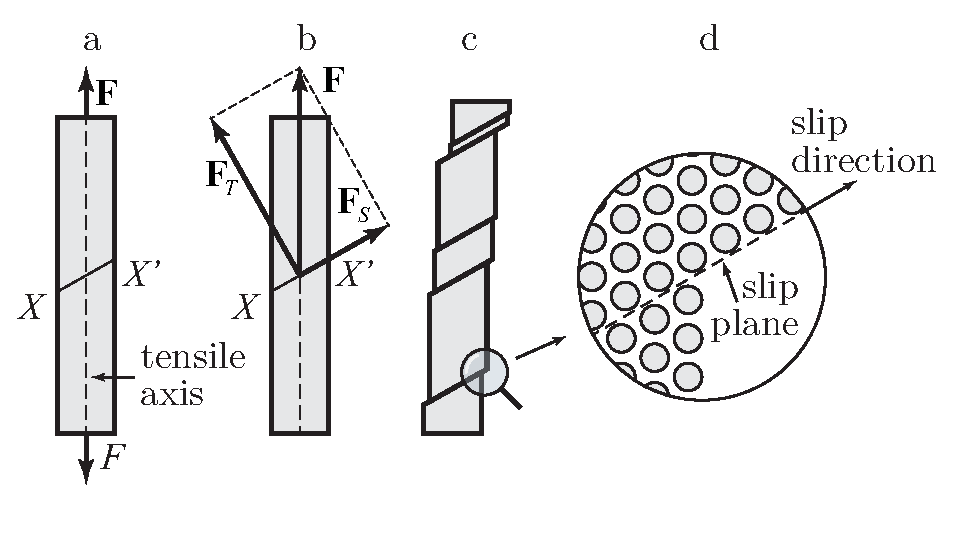
\includegraphics[width=0.6\textwidth]{slip_mechanism}
\caption[Plastic deformation]{The slip mechanism in plastic deformation.}
\label{fig:plastic_deformation}
\end{figure}

\subsection{The role of dislocations in modelling plasticity}
In engineering, plastic deformation is often described by phenomenological models in which constitutive relations are given between the stress, deformation, deformation rate and dislocation density\cite{Taylor1938307,HILL1972401,ASARO1985923,KUBIN1985397}. These models provide satisfactory results for a large variety of materials under general conditions for large enough samples. It turned out, however, that on a \si{\micro\meter} size scale the mechanical properties and the general behaviour of crystalline materials differ from what their phenomenological theories can predict \cite{FLECK1994475,mcelhaney_vlassak_nix_1998,Csikor251}. One example is the system size dependence of the plastic response observed experimentally, that is called size effect and it plays an important role in nanotechnology.

Due to the intense development in nanotechnology, it was inevitable to face the challenges of size effec to develop models correctly describing and modelling specimens in the \si{\micro\meter} size scale. The pressure from the side of the industry first led to the developement of new phenomenological, non-local models that describe the size effect successfully \cite{FLECK1994475,WalgraefAifantisJournal,WALGRAEF19851365}. However, they neglect the fact that plastic deformation are achieved by the motion of individual dislocations. They introduce gradient terms with coefficients containing length-dimensional parameters leading to a fundamental confrontation with the properties  of dislocations (see appendix \ref{sec:dimensionless_units}). These models are capable for capturing the hardening due to the smaller size of the specimen and they also explain some types of dislocation patterning, but due to their fundamental approach they are unable to account for some other phenomenon involving to involve the mechanism of dislocations. It has turned out that the plastic deformation of micropillars (micron-sized single crystal rods) is realised by intermittent, avalanche-like strain bursts in different regions of the sample as seen in Fig.~\ref{fig:avalanches_EM} \cite{DIMIDUK20054065,Dimiduk1188,Csikor251}. This behaviour makes the phenomenological models inefficient in predicting the plastic deformation on nanoscale.

\begin{figure}[htbp!] 
\centering    
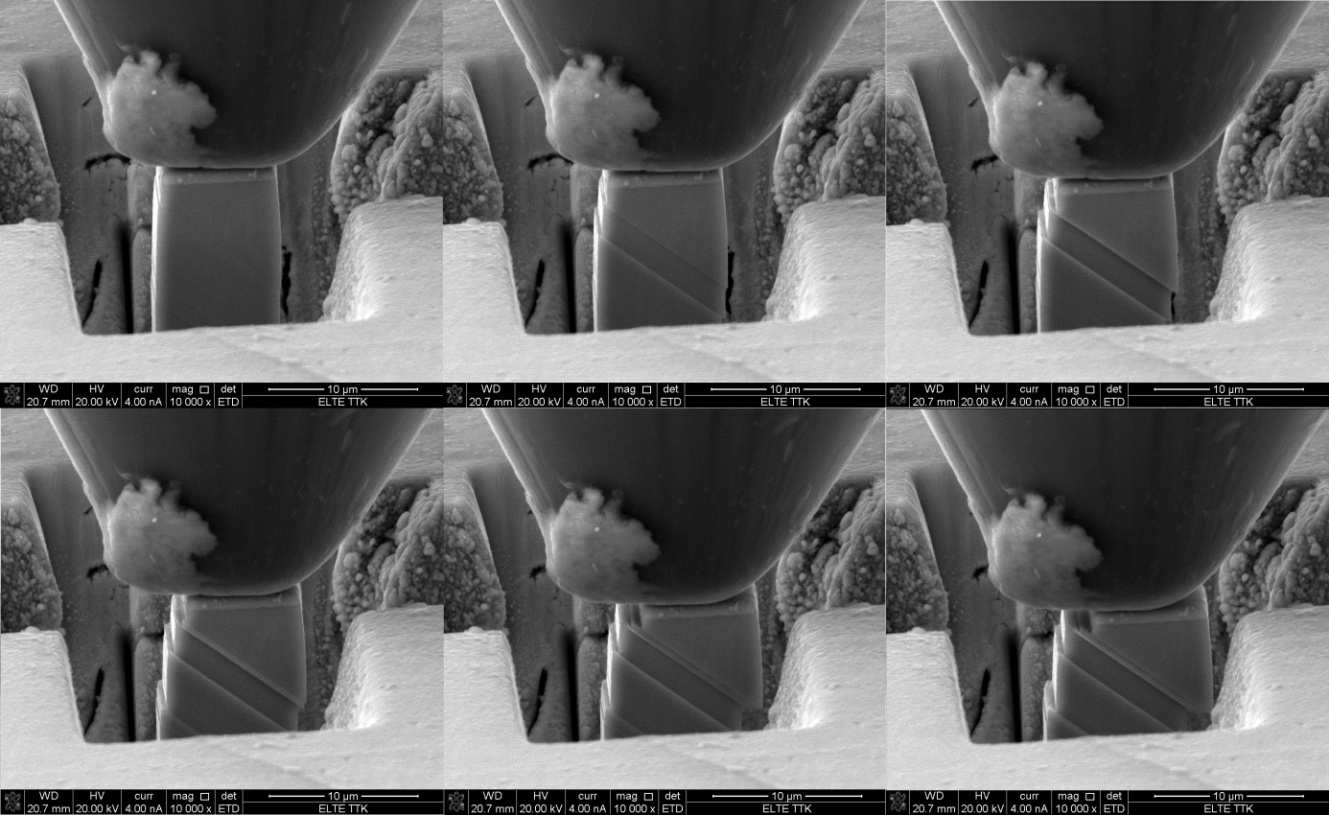
\includegraphics[width=0.8\textwidth]{bazalisZn28840.png}
\caption[Plastic deformation on nanoscale]{The slip mechanism in plastic deformation on nanoscale. The plastic response is not continuous, as it would be expected on macroscales. This picture has been taken at ELTE in a scanning electron microscope of a Zn single crystal oriented to basal slip system.}
\label{fig:avalanches_EM}
\end{figure}

\nomenclature[z-FIB]{FIB}{focused ion beam}      % first letter Z is for abbreviation
\nomenclature[z-CA]{CA}{cellular automaton}

%\nomenclature[a-F]{$F$}{complex function}                                                   %% first letter A is for Roman symbols

%\nomenclature[g-p]{$\pi$}{ $\simeq 3.14\ldots$}                                             %% first letter G is for Greek Symbols
%\nomenclature[g-i]{$\iota$}{unit imaginary number $\sqrt{-1}$}                      %% first letter G is for Greek Symbols
%\nomenclature[g-g]{$\gamma$}{a simply closed curve on a complex plane}  % %first letter G is for Greek Symbols
%\nomenclature[x-i]{$\oint_\gamma$}{integration around a curve $\gamma$} % %first letter X is for Other Symbols
%\nomenclature[r-j]{$j$}{superscript index}                                                       %% first letter R is for superscripts
%\nomenclature[s-0]{$0$}{subscript index}                                                        %% first letter S is for subscripts


%********************************** %Second Section  *************************************
\section{The actuality of the topic} %Section - 1.2

As described above, plastic strain is realised by and can be described with a fundamentally new mechanism in the regime of submicron scales. That is, the collective motion of dislocations causes a large intermittent strain burst -- called dislocation avalanches -- that in turn accumulates and creates plastic strain. This noisy behaviour can be handled only by statistical approaches.

The actuality of the topic is two-fold. First, state-of-the-art computers are able to run simulations on a much larger scale than ever before. Large supercomputers are capable to run molecular dynamic\footnote{See section \ref{sec:disloc_sim_md_sim}} simulations on \num{1000 x 1000 x 1000} atoms, displaying the core properties of dislocations in 3D. One cannot expect, however, that any of these computers can simulate a sample with size scale of \si{\micro\meter}. Simulations where the elementary units are the dislocations (or their segments) are also developed. They can capture the collective, avalanche-like behaviour of dislocations. Such models with further simplifications (e.g.\ 2D simulations) can be well handled on a larger computers that many universities and their departments have at their disposal.\footnote{These simplifications are still not sufficient in order to simulate a micron-sized sample. Consider a simulation with a mean dislocation density of \SI{e14}{\per m^2} in a micron-sized sample. In this case, one has to face \si{10^8} number of dislocations interacting with $10^8-1$ number of dislocations leading to a total of ${10^{16}}/2$ number of pair-interaction calculations per time steps. Supposing a lightning-fast CPU -- with a frequency of \SI{10}{\GHz}), and supposing that in each tick cycle the strongness of a pair-interaction force out of the $N^2/2$ can be calculated -- the time scale required to calculate all pair-interactions for just one single time step is in the order of months. Although this strong underestimation can be improved with parallel computing by involving hundred thousands of processors, the strong physical simplifications and huge technological challenges question the profitability of such trials.}

Second, state-of-the-art nanotechnology nowadays allows us to fabric and manipulate samples with a technology called FIB (focused ion beam) on the size scale of \si{\micro\meter}, on which the plastic deformation of the sample is deeply on the submicron scale. One can therefore recognise that nowadays the size scale one can simulate and fabric are in the same order of magnitude. This new key feature of the field has increased the possibility to verify models directly by physical, real specimen measurements and measurements can be suggested based on the results of computer simulations. Until now a large drawback of the technology was that the samples prepared with FIB in the vacuum chamber of the SEM were not deformed in the same device due to technical problems. Technological advancement also let us to develop a nanodeformation tool that can fit into the vacuum chamber of a SEM, facilitating to investigate in situ the emerging steps on the side of miropillars formed due to dislocation avalanches.

%********************************** % Third Section  *************************************
\section{The structure of the thesis}
In the next chapter, models describing crystal defects are presented with the focus on dislocation simulations, especially on continuum dislocation simulations. This is necessary in order to understand the models introduced in the latter parts.

The objective of this thesis is two-fold, just as the actuality of the topic. 
In the first half of the thesis, the topic is approached from a simulation point of view in chapter \ref{chapter:weakest_link}. A cellular automaton (CA) model is introduced to link model parameters between discrete dislocation dynamics \nomenclature[z-DDD]{DDD}{discrete dislocation dynamics}(DDD) and continuum dislocation dynamics (CDD) \nomenclature[z-CDD]{CDD}{continuum dislocation dynamics} models. The results are published in an article noted in chapter \ref{chapter:publications}, at point \hyperref[paper:A2]{[O1]}. A remarkable feature of the numerical model is that with further extensions of the CA model it is capable of describing materials which undergo strain softening, like metallic glasses. A striking property of the model, is that it is capable of describing single crystals just as metallic glasses. The details are described in the chapter \ref{chapter:disorder}, in which this feature is utilised to study fracture under strain softening in metallic glasses. The results are published in a paper, at point \hyperref[paper:A3]{[O2]} in chapter \ref{chapter:publications}. Finally, another CA model is introduced in chapter \ref{chapter:pattern} to study dislocation patterning. The results are presented along with a non-discretised model. The results have been also published in a paper, noted at point \hyperref[paper:A4]{[O3]} in chapter \ref{chapter:publications}.

In the second half, the topic of this thesis is approached from an experimental point of view, see chapter \ref{chapter:in_situ}. In order to investigate the properties of plastic deformation on a micron-scale, one has to produce a mass amount of samples and test them. The fabrication can be done by a FIB, a commercially available technology for electron microscopes. Another challenge is how to construct and calibrate a nanodeformation device (which fits into the vacuum chamber of a SEM) in order to conduct experiments. The device is coupled to an acoustic emission signal detector to exhibit the potential of the setup. The results achieved therewith has been already published in a paper, see point \hyperref[paper:A1]{[O4]} in chapter \ref{chapter:publications}.
%!TEX root = ../thesis.tex
%*******************************************************************************
%****************************** Second Chapter *********************************
%*******************************************************************************

\chapter{Dislocation simulations}

\ifpdf
    \graphicspath{{Chapter2/Figs/Raster/}{Chapter2/Figs/PDF/}{Chapter2/Figs/}}
\else
    \graphicspath{{Chapter2/Figs/Vector/}{Chapter2/Figs/}}
\fi


\section{From molecular dynamics to discrete dislocation dynamics}

In materials science and physics, modeling and simulation play an essential role. In engineering knowledge-based tools are developed to design materials with better performance without unnecessary trials. They are used for quantitative understanding on the relations between composition, processing, structure and properties of the materials. From the materials physics point of view there are great possibilities to test early concepts to describe qualitative findings. Although tremendous potential benefits of modeling and simulation are brought to mankind, they pose challenges because of the huge complexity involving multiple orders of magnitude in time and space scales, mentioning only one of the toughest.
\begin{enumerate}
\item Dislocations bring a clear example of the size scale problems. Dislocation patterning appears on the size scale of hundreds of mean dislocation spacing 
($ \approx $ \SI{10}{\um}), while to resolve dislocation core structure scales below atomic distance are needed
(less than \SI{1}{\angstrom}).
\item Due to the long range interaction the collective motion of dislocation involves rather different different time scales. Creep is a rather slow deformation while the timescale of dislocation motion is short range. This challenge arises e.g.\ at simulating dislocations in single crystal Ni-based superalloys used in aircraft turbine blades: the timescale of dislocation motion is in the order of \si{\us}, while the change in microstructures happens in the order of weeks.
\end{enumerate}
Moreover chemical interactions may play a non-negligible role too. Covering interdisciplinary phenomena whose modelling involves different approaches elevate the problem to a conceptual level. Despite all these difficulties computational models show fruitful promises worth to try. As a general principle the physical accuracy of a model and its practicability are opposite aims regarding the spatial and temporal scales. So minimalist models introducing the smallest possible number of parameters by identifying the essential mechanisms which can capture the phenomenon desired are essential.\footnote{That's why I consider keyboard pushing as science when it comes to simple models based on physical assumptions.}

\subsection{Ab initio}
The starting point of the most fundamental picture in materials' simulation are the wave functions of the nuclei and electrons. ``Schrödinger's equation may solves all\footnote{Richard Feynmann: Lecture on Physics, Volume II, 41–6: Couette flow}'' and describe the time evolution of the system on the level of quantum physics. These models may involve Hartree-Fock and density functional theory approximation, but a key feature is that no phenomenological parameters are introduced. These first principle methods (also known as ab initio) represents the state of the art, completely non-phenomenological methods. First principle methods let us to construct materials have not created yet. It allows to investigate their parameters leading to an improvement in efficiency compared to a completely trial and error experimental discovery of new materials. Due to the complexity of the Schrödinger's equation simulations are strongly limited in both the number of independent variables (particles) and the time length. Their typical values are around \textbf{\numrange{1}{100} atoms} and time range of \textbf{\SIrange{e-15}{e-12}{\second}}. These limitation mean that ab initio methods cannot be used to study the collective properties of dislocations, but the properties of the primitive cell and crystal lattice as the underlying structure for dislocations.

\subsection{Molecular modelling} \label{sec:disloc_sim_md_sim}
Atomic scale methods consider atoms as the smallest units and are essentially build upon the equations of classical mechanics. They do not resolve subatomic scales, i.e.\ nuclei and electrons and their effect taken into account via phenomenological parameters as input parameters of the model leading to the possibility to simulate materials different in structure or in chemical properties. Limitations are moderated compared to ab initio methods: \textbf{\numrange{e4}{e9} or even up to \num{e12} number of atoms} can be handled for up to \textbf{\SIrange{e-12}{e-9}{\second}}. Atomistic methods can be casted into two major categories:
\begin{enumerate}
\item stochastic methods such as Monte Carlo methods\cite{alfonso2015simulation,saito1997monte},
\item deterministic methods such as molecular dynamics (MD\nomenclature[z-MD]{MD}{Molecular dynamics}). MD simulations are capable to simulate dislocation-related properties, such as dislocation-solute atom interaction, interface-matrix dislocation interaction and dislocation-dislocation interaction, creation, and annihilation \cite{ZHANG2013132,doi:10.1080/14786430903081990,Yamakov2002}. Due to computational limitations, they cannot handle large number of dislocations or very slow effects, e.g.\ deformation with a slow strain rate and diffusion controlled processes (like dislocation-climb).
\end{enumerate}

\subsection{Xscopic scale methods}
It is common to distinguish models corresponding to different scales as microscopic, mesoscopic, and macroscopic (denoted by my fantasy name xscopic) scales. They are above atomic scale methods' but their naming is rather arbitrary or field-dependent. Macroscopic scales means the size scale where materials can be handled homogeneous and all phenomena related to atoms can be taken into account via a finite number of parameters and where completely classical approaches can be used. In practice this scale is in the order of \si{\milli\meter} and above. Microscopic scale is directly above atomic scales where ab initio and MD are used. Mesoscale is something in between. In the field of phase/grain microstructures "microscopic" stands for intraphase/intragrain scales and mesoscopic stands for interphase/intergrain scales\cite{Rotersbook}. In fields of dislocation microscopic means that individual dislocations can be resolved (discrete dislocation) and mesoscopic means field quantities (e.g.\ dislocation density or dislocation-dislocation two particle correlation) are introduced to handle dislocated-related phenomena. The work presented in the thesis focuses on dislocations therefore the latter terminology is utilised in the following.

\textbf{Microscopic} methods in this sense mean discrete models like DDD where dislocations resolved into segments along the dislocation line. Forces -- including driving forces, dissipative forces and inertial term -- acting on the whole dislocation is averaged for the segments determining the motion of the segments. Driving force may include various sources, such as external force, dislocation-interaction forces ... etc. DDD simulations provide information on each of the dislocation and they can also handle large number of dislocations even in multiple slip systems to study their evolution during rearrangement. Larger number of dislocations means that with some simplifying assumptions commercially available computers can catch collective dislocation motion phenomena, such as dislocation avalanches \cite{Csikor251,ovaska2015quenched,PhysRevLett.112.235501}. A strong drawbacks of DDD simulations is a trivial outcome of their approach: they resolve dislocations one by one. So since one tries to track the motion of each dislocation segment, the problem leads to computational cost unaffordable at the scales of dislocation patterning.

\textbf{Mesoscopic} methods average out the microstructure: they refers to such models where  fields and continuum quantities are used. As an example, DDD resolved each of the dislocations and tracks their motion, while in CDD modelling dislocation density distributions, dislocation-dislocation correlation functions ... etc. are introduced and their change in time describes the evolution of the system. As a consequent, their computational cost is basically independent of the number of dislocations (or dislocation density) therefore simulation space can be scaled up even to the size scale where real specimen experiments can be performed even on commercial computers. While in DDD models the way stresses are calculated is more or less straightforward, CDD models lead to nontrivial conceptual problems: what are the key quantities, how to handle them mathematically and how could one handle efficiently to a numerical problem. This challenge is not surprising, because CDD models have to link
\begin{itemize}
\item information got from lower-levels contained in discrete models, like the microstate of dislocations and
\item information got from higher-levels describing materials on macroscopic scales.
\end{itemize}
The difficulties mentioned above can be handled by deriving terms and numeric parameters in a continuum models obtained by coherent coarse graining of discrete models. The expected results can be also foreseen by empirically generalise the experimental data in an an adequate way.

\textbf{Macroscopic} scale methods approach the problem from the opposite direction. In this case the evolution of the whole system is prescribed phenomenologically and only finite amount of averaged parameters are used to account for the microstructure. The main advantage of these models is that their numeric implementation is straightforward, they can easily fit into the standard framework of finite element methods already available. These models are efficient engineering tools when it comes to estimate the life-time \cite{Connolly_2014_MST, Le_2014_IJP} under mechanical fatigue or creep conditions. In experiments the details of the stress-strain curves are highly dependent on the specific test conditions hence model parameters must also reflect this sensitivity feature if the underlying constitutive formulation still holds at all. These methods are reliable only in a limited range where they are tested against real experiments meaning their prediction can hardly go beyond what the models were build upon. They are able to capture, however, changing microstructural mechanism by using new set of parameters, i.e.\ introducing new ones and omitting old ones, but this is barely a phenomenological approach where one can hardly give the parameters used in the model any microstructural meaning. Although no doubt that these models provide useful tools in their own field of engineering, they are inadequate for the field of microstructure engineering.


\section{Contiuum dislocation dynamics} \label{sec:disloc_sim_CDD}
The basis of continuum dislocation dynamics was founded by Nye and Kröner in the nineteen fifties by introducing a tensorial measure, the Kröner-Nye dislocation density tensor to represent the geometrically necessary dislocation (GND) \nomenclature[z-GND]{GND}{geometrically necessary dislocation} densities in a crystal. It was cumbersome and took half a decade to describe plasticity with the density field  introduced above in a nontrivial case of continuous dislocation density where one has to already take into account the boundary conditions \cite{doi:10.1080/14786436308213841}. Since then numerous different models based on the Kröner-Nye tensor were introduced \cite{Acharya_2001_JMPS, Le_2016_IJP, Sedlacek_2003_PM, Xia_2015_MSMSE} where dislocations are the boundaries between plastically sheared and unsheared regions on a slip plane. In this picture all dislocations are geometrically necessary and there's no other type of dislocation. In energy functional based models (such as phase field dislocation dynamics model \cite{Beyerlein20150166}) dislocation evolution is driven by the decreasement of the total internal energy, therefore any other source of dislocations than the boundary is neglected. These models can hardly resolve the system spatially below the mean dislocation distance meaning they are inadequate models to account for mechanisms taking place below this size scale.

Another possible type of dislocation is the statistically stored dislocation (SSD) density \nomenclature[z-SSD]{SSD}{statistically stored dislocation} accounted only for the flow stress and plastic slip rate. It neglects completely the geometric compulsion \cite{johnston_1959_JAP, Kocks_1976_JEMT}. These models focus on the reproduction of the connection between dislocation density and the flow stress (e.g.\ the Taylor-equation for the flow stress ${\tau _f} = \alpha GB\sqrt \rho  $, where $G$ is the shear modulus) and the connection between the plastic slip rate (e.g.\ the Orowan-equation $\partial \eta /\partial t = \rho vb$, where $\eta$ is the plastic strain). These descriptions are valid as long as the naive picture of dislocations holds\footnote{tautology} and in these cases they can also describe work hardening and plastic flow \cite{Bouaziz_2013_PM, Caceres_2007_MSEA, Estrin_1984_AM} on a phenomenological base.

In the rest of this work we will focus on another line of approach where individual dislocations are coarse grained only of its own type. These models can account for the evolution of GND and SSD simultaneously \cite{Groma_1997_PRB, Groma_2003_AM}. To minimalise the complexity of such model one could consider only straight edge dislocations in a plain-strain geometry where only two types of dislocations exist: with Burgers vector $s \cdot b$, $s \in \left\{ { +1 , -1 } \right\}$, called 2D dislocation model\footnote{The 3rd direction, $z$, is in the direction of the dislocation line.}. Although the explanation and interpretation of the appearing term in 2D CDD models \cite{Groma_2003_AM} reveals astonishing features \cite{PhysRevB.93.214110}, arbitrary configurations of curved dislocations became examinable with a general extension \cite{Hochrainer_2014_JMPS, hochrainer2007three, Stefan_2011_JMR, SANDFELD20151} granted by a straightforward though cumbersome calculation applied on the original basis. These models have been successfully tested against DDD simulations \cite{Stefan_2015_MSMSE} or against other CDD models \cite{Monavari_2016_JMPS} and proved to be accountable on the size scale below the mean dislocation spacing up to orders of magnitude larger scales.

In the following an above-mentioned 2D CDD model with a statistical approach will be introduced in order to present the basis of chapter \ref{chapter:weakest_link} and \ref{chapter:pattern}.

\subsection{Equation of motion of dislocations}
\nomenclature[z-EOM]{EOM}{equation of motion}
In this section the equation of motion (EOM) of straight, parallel edge dislocations in single slip is discussed from a DDD point of view. This is the simplest setup one can envisage which still reproduces some key features of dislocation system demonstrated by DDD simulations. The derivation is implemented by a systematic manner providing further possibilities for improvement.


\begin{figure}[htbp!] 
\centering    
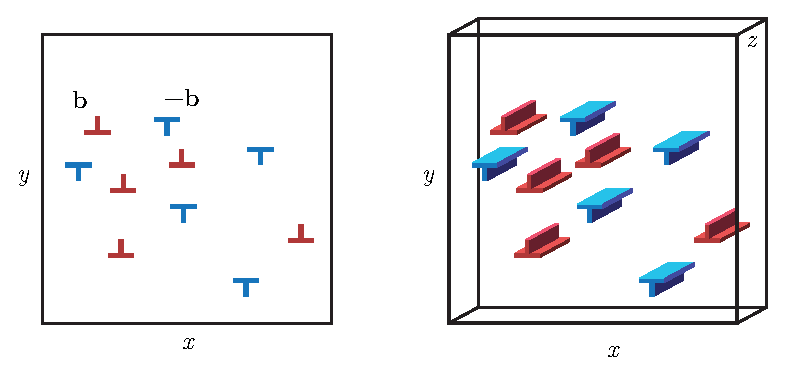
\includegraphics{DDD2}
\caption[2D DDD]{A 2D dislocation configuration (single slip) representing a total of $N = N_t = 10$ dislocations; ${N_ + } = 5$, ${N_ - } = 5$, the number of exceed dislocations ${N_s} = \sum\limits_{i = 1}^N {{s_i}}  = 0$ (s for signed). The $z$ direction is perpendicular to the plane of the sheet/screen and points towards the reader. (The $x$, $y$ and $z$ axes form a right-handed system.)}
\label{fig:2D_DDD}
\end{figure}

In the following we consider $N$ dislocations with Burgers vector $s \cdot \left( {b,0,0} \right)$, $s \in \left\{ { - 1,1} \right\}$ with dislocation line directing to the positive direction of the $z$ axis (see Fig.~\ref{fig:2D_DDD}). Neglecting the inertial terms on dislocations, i.e.\ using over-damped dynamics, the EOM of the dislocation system is given by
\begin{equation} \label{eq:EOM_DDD}
\frac{{d{x_i}}}{{dt}} = {M_0}b{s_i}\left( {\sum\limits_{j = 1}^N {{s_j}{\tau _{{\text{ind}}}}\left( {{{\mathbf{r}}_i} - {{\mathbf{r}}_j}} \right) + {\tau _{{\text{ext}}}}} } \right),
\end{equation}
where ${{\mathbf{r}}_i} = \left( {{x_i},{y_i},{Z_i}} \right)$ is the position ($Z_i$ points to the points of the dislocation line), ${s_i}$ is the sign of the $i$th dislocation, $M_0$ is a mobility factor specific to the dislocation in the system given, $b_i$ is the Burgers vector, ${{\tau _{{\text{ind}}}}}$ is the shear stress generated by dislocation $j$ at the place of dislocation $i$, ${{\tau _{{\text{ext}}}}}$ is the external shear stress. For simplicity the time dependence of ${{\mathbf{r}}_i}$ will not be indicated in the rest of this thesis. The actual form of ${\tau _{{\text{ind}}}}$ reads as
\begin{equation} \label{eq:tau_ind}
{\tau _{{\text{ind}}}}\left( {\mathbf{r}} \right) = x\frac{{{x^2} - {y^2}}}{{{{\left( {{x^2} + {y^2}} \right)}^2}}} = \frac{{\cos \left( \phi  \right)\cos \left( {2\phi } \right)}}{r}.
\end{equation}

By adding a random force term to \cref{eq:EOM_DDD}, the model is capable to contain the effect of thermal noise, leading to a stochastic differential equation. By investigating the corresponding Fokker-Planck equation with real physical parameters, one can find that the time scale corresponding to thermal noises are orders of magnitude (e.g.\ $10^4$) larger then the one corresponding to dislocation-dislocation interaction. Neglecting the thermal fluctuation in the elastic energy resulting that the dislocations cannot escape from even the smallest energy barrier leaving them in the nearest local energy minimum. One has to note that although dislocations are still unstable crystal defects meaning that dislocation-free system would be the preferred configuration, this state cannot be achieved because the system cannot recover from its metastable configuration -- at least within a reasonable time.

Dislocation climb is another thermal effect could have been taken into account. The underlying mechanism lies on vacancies which are stable crystal defects at finite temperature. However, in the followings dislocation climb will be neglected and only glide will be allowed representing a zero-temperature approximation.

\subsubsection{Coarse graining}
The first step towards the desired CDD model from the DDD model is the procedure called coarse graining or homogenisation. The dislocation density tensor introduced by Nye and Kröner is
\begin{equation}
{\alpha _{ij}} =  - {\varepsilon _{ikl}}{\partial _k}\beta _{lj}^{\text{p}},
\end{equation}
where 
$\varepsilon $ is the three-dimensional Levi-Civita symbol\footnote{The completely antisymmetric $3 \times 3 \times 3$ tensor, or the three indexed permutation symbol} and $\beta _{lj}^{\text{p}}$ is the plastic distortion. In the 2D single slip case the quantity ${\alpha _{ij}}$ has only one non-zero component, and it is highly singular on a DDD level: it can be written as a sum of Dirac-delta distributions
\begin{equation} \label{eq:alpha_is_sum_of_dirac_delta}
{\alpha _{31}} = {\rho _{\text{d}}} = \sum\limits_{i = 1}^N {{s_i}\delta \left({{\mathbf{r}} - {{\mathbf{r}}_i}} \right)},
\end{equation}
where ${\rho _{\text{d}}}:{\mathbb{R}^2} \to \mathbb{R}$ denotes the scalar-valued dislocation density. The evolution of the system is completely defined at this point: the EOM of the dislocations are given meaning that the dislocation density can be calculated at any give point at any time which determines -- compared to an initial state -- the plastic distortion and the stress. In this case, however, one has to follow each of the dislocation containing the whole microscopic information of dislocation configuration.

In a hopefully lucky situation one may predict the macroscopic plastic response of the system without knowing the detailed information of the whole dislocation arrangement and the vast majority of the information can be neglected by finding the key homogeneous quantities as it is done in many other physical systems. One way to do that is to calculate locally averaged fields for the dislocation density, dislocation current density, stress, ... etc. Locally averaged means that a convolution is applied with a window function tending to zero fast enough in a certain sense. One may ask if there are only one appropriate function or more, which ones are better and worse and if there exist any window function at all which could provide averaged quantities modelling our system. There is a hope that within certain limits a range of function do the job and the main features of the result obtained by coarse graining does not depend strongly on the specific shape of the window function. If we cannot find any proper function and our model seems to be ineffective describing the reality it may mean that all the microscopic details are necessary for the description and one cannot use a continuum picture.

The goal of the continuum description is to get rid of unimportant details to speed up the numerical models implemented on such basis. However, one has to be careful. Consider two dislocation configurations where signed sum of dislocations are equal within a region, ${N_s} = \sum\limits_{i = 1}^N {{s_i}} $, as seen in Fig.~\ref{fig:coarse_graining}. Apply coarse graining with a window function with the size of box. Consider the signed dislocation density $\kappa$. It can be seen that on one hand the value of $\kappa$ are the same and on the other hand the plastic response of the two configurations are substantially different. This is an example to point out that further quantities than dislocation density tensor is needed to characterise the state of the system.

\begin{figure}[htbp!] 
\centering    
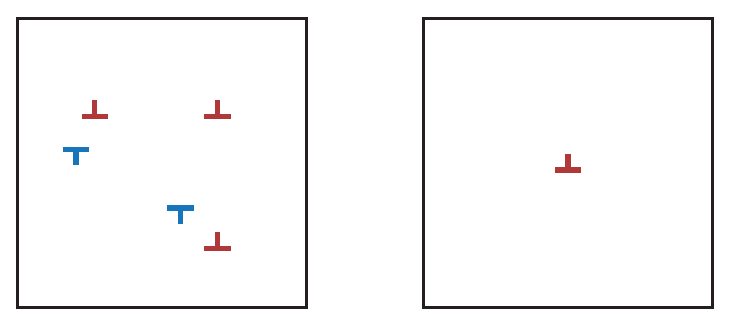
\includegraphics[width=0.8\textwidth]{coarse_graining}
\caption[Coarse graining is riskful]{Coarse graining applied on strongly different dislocation arrangement can lead to the same signed dislocation densities at some points. This two configurations gives the same signed dislocation density $\kappa$ at the center using a window function represented by the box.}
\label{fig:coarse_graining}
\end{figure}


To introduce the key quantities under certain assumptions one has to coarse grain the EOM in \cref{eq:EOM_DDD}. For shorter notation only $s_i=+1$ type of dislocations will be considered first and then the results obtained will be generalised to the case when two types of dislocations are presented. For simplicity, ${\tau _{{\text{ext}}}}$ is neglected first. Let us apply ${\partial _x}\left( {\delta \left( {{\mathbf{r}} - {{\mathbf{r}}_i}} \right) \cdot  \bullet } \right)$ first on both sides:
\begin{equation} \label{eq:EOM_DDD2}
{\partial _x}\left[ {\frac{{d{x_i}}}{{dt}}\delta \left( {{\mathbf{r}} - {{\mathbf{r}}_i}} \right)} \right] = {M_0}{\partial _x}\left\{ {\left[ {\sum\limits_{j \ne i}^N {F\left( {{{\mathbf{r}}_i} - {{\mathbf{r}}_j}} \right)} } \right]\delta \left( {{\mathbf{r}} - {{\mathbf{r}}_i}} \right)} \right\},
\end{equation}
where $F\left( {\mathbf{r}} \right) = b \cdot {\tau _{{\text{ind}}}}\left( {\mathbf{r}} \right)$. With the equivalency
\begin{equation}
{\partial _x}\left( {\frac{{d{x_i}}}{{dt}}\delta \left( {{\mathbf{r}} - {{\mathbf{r}}_i}} \right)} \right) = \frac{{d{x_i}}}{{dt}}{\partial _x}\delta \left( {{\mathbf{r}} - {{\mathbf{r}}_i}} \right) =  - \frac{{d{x_i}}}{{dt}}{\partial _{{x_i}}}\delta \left( {{\mathbf{r}} - {{\mathbf{r}}_i}} \right) =  - \frac{d}{{dt}}\delta \left( {{\mathbf{r}} - {{\mathbf{r}}_i}} \right)
\end{equation}
\cref{eq:EOM_DDD2} reads as
\begin{equation}
 - \frac{d}{{dt}}\delta \left( {{\mathbf{r}} - {{\mathbf{r}}_i}} \right) = {M_0}{\partial _x}\left[ {\left\{ {\int {F\left( {{\mathbf{r}} - {\mathbf{r}}'} \right)} \left[ {{\rho _{\rm{d}}}\left( {{\mathbf{r}}'} \right) - \delta \left( {{\mathbf{r}} - {\mathbf{r}}'} \right)} \right]{d^2}r'} \right\}\underbrace {\delta \left( {{\mathbf{r}} - {{\mathbf{r}}_i}} \right)}_{{\text{avoid self - int}}{\text{.}}}} \right].
\end{equation}
Here the term ${\delta \left( {{\mathbf{r}} - {{\mathbf{r}}_i}} \right)}$ is to avoid self interaction of the dislocations. Recall \cref{eq:alpha_is_sum_of_dirac_delta} and take into account that only positive dislocations are considered and sum up both sides with respect to $i$:
\begin{equation}
 - \frac{d}{{dt}}{\rho _{\rm{d}}}\left( {\mathbf{r}} \right) = {M_0}{\partial _x}\left[ {\left\{ {\int {F\left( {{\mathbf{r}} - {\mathbf{r}}'} \right)} \left[ {{\rho _{\rm{d}}}\left( {{\mathbf{r}}'} \right) - \delta \left( {{\mathbf{r}} - {\mathbf{r}}'} \right)} \right]{d^2}r'} \right\}{\rho _{\rm{d}}}\left( {\mathbf{r}} \right)} \right].
\end{equation}
Please note the non-local property of this equation. Let us make the coarse graining now by applying the operation
\begin{equation}
\left\langle { \bullet \left( {\mathbf{r}} \right)} \right\rangle  = \int { \bullet \left( {{\mathbf{r}}'} \right) \cdot w\left( {{\mathbf{r}} - {\mathbf{r}}'} \right){d^2}r'}  = \left( { \bullet  * w} \right)\left( {\mathbf{r}} \right).
\end{equation}
Denote the averaged one-particle dislocation density function by
\begin{equation} \label{eq:intro_one_particle}
{\rho _1}\left( {\mathbf{r}} \right) = \left\langle {{\rho _{\rm{d}}}\left( {\mathbf{r}} \right)} \right\rangle,
\end{equation}
and the two-particle dislocation density by 
\begin{equation} \label{eq:intro_two_particle}
{\rho _2}\left( {{{\mathbf{r}}_1},{{\mathbf{r}}_2}} \right) = \left\langle {{\rho _{\rm{d}}}\left( {{{\mathbf{r}}_1}} \right){\rho _{\rm{d}}}\left( {{{\mathbf{r}}_2}} \right) - {\rho _{\rm{d}}}\left( {{{\mathbf{r}}_1}} \right)\delta \left( {{{\mathbf{r}}_1} - {{\mathbf{r}}_2}} \right)} \right\rangle.
\end{equation}
With these notation one gets
\begin{equation} \label{eq:one_two_particle_EOM}
\frac{{\partial {\rho _1}\left( {\mathbf{r}} \right)}}{{\partial t}} + M_0 \int {{\partial _x}\left[ {{\rho _2}\left( {{\mathbf{r}},{{\mathbf{r}}_2}} \right)F\left( {{\mathbf{r}} - {{\mathbf{r}}_2}} \right)} \right]{d^2}{r_2} = 0}.
\end{equation}
Please note that in this equation ${\rho _1}\left( {\mathbf{r}} \right)$ and ${\rho _2}\left( {{{\mathbf{r}}_1},{{\mathbf{r}}_2}} \right)$ represent the coarse-grained one- and two-particle densities.

\Cref{eq:one_two_particle_EOM} does not describe completely the system, it contains two time-dependent values ${\rho _1}\left( {\mathbf{r}} \right)$ and ${\rho _2}\left( {{{\mathbf{r}}_1},{{\mathbf{r}}_2}} \right)$. This equation could be used to express the time evolution of the one-particle density function dependent on two-particle density function. However, one can get an equation for the two-particle density function depending on the three-particle density function, ... etc, and in the end the $N-1$-particle density function will depend on the $N$-particle density function. The general equation that gives the dependence of the $k$-particle density function on the $N>k$ particle density function can be found in the work of \citet{Groma_1997_PRB}:
\[\frac{{\partial {f_k}}}{{\partial t}} + \sum\limits_{i = 1}^k {\sum\limits_{j = i,j \ne i}^k {{\partial _{{x_i}}}\left[ {{f_k} \cdot F\left( {{{\mathbf{r}}_i} - {{\mathbf{r}}_j}} \right)} \right]} }  + \left( {N - k} \right)\int {{\partial _{{x_i}}}\left[ {{f_{k + 1}} \cdot F\left( {{{\mathbf{r}}_i} - {{\mathbf{r}}_{k+1}}} \right)} \right]d^2{r_{k + 1}}}  = 0,\]
where the $k$-particle distribution function is introduced, ${\rho _k} = \frac{{N!}}{{k!}}{f_k}$, and it is a function of the coordinates of the dislocations,${f_k}\left( {{{\mathbf{r}}_1},{{\mathbf{r}}_2},...,{{\mathbf{r}}_k}} \right)$, and of the time as well.

With these one got a hierarchy of equations. This form is still equivalent with the description of the original DDD system without the loss of generality, because nothing is supposed on the window function appearing only in the $i$-particle density functions (namely the ${\rho _1}\left( {\mathbf{r}} \right)$ and ${\rho _2}\left( {{{\mathbf{r}}_1},{{\mathbf{r}}_2}} \right)$ in \cref{eq:intro_one_particle,eq:intro_two_particle}). This generality breaks off when one gives a specific function on $w$. In the next two sections different approximation are applied on these terms. It turns out that at least the first  one -- the self-consistent, or mean field -- is an oversimplification while the latter one provides enough to observe dislocation avalanches and dislocation patterning. Before we do so, let us generalise the form of \cref{eq:one_two_particle_EOM} for two different types of dislocations: one with Burgers vector $+b$ and one with $-b$ pointing to the $x$ direction.
\begin{equation} \label{eq:intro_pos_EOM}
\frac{{\partial {\rho _ + }\left( {\mathbf{r}} \right)}}{{\partial t}} =  - {M_0}b{\partial _x}\left\{ {\int {\left\{ {\left[ {{\rho _{ +  + }}\left( {{\mathbf{r}},{{\mathbf{r}}_2}} \right) - {\rho _{ +  - }}\left( {{\mathbf{r}},{{\mathbf{r}}_2}} \right)} \right]{\tau _{{\text{ind}}}}\left( {{\mathbf{r}} - {{\mathbf{r}}_2}} \right)} \right\}{d^2}{r_2}}  + {\rho _ + }\left( {\mathbf{r}} \right){\tau _{{\text{ext}}}}} \right\}
\end{equation}

\begin{equation} \label{eq:intro_neg_EOM}
\frac{{\partial {\rho _ - }\left( {\mathbf{r}} \right)}}{{\partial t}} =  - {M_0}b{\partial _x}\left\{ {\int {\left\{ {\left[ {{\rho _{ -  - }}\left( {{\mathbf{r}},{{\mathbf{r}}_2}} \right) - {\rho _{ -  + }}\left( {{\mathbf{r}},{{\mathbf{r}}_2}} \right)} \right]{\tau _{{\text{ind}}}}\left( {{\mathbf{r}} - {{\mathbf{r}}_2}} \right)} \right\}{d^2}{r_2}}  - {\rho _ - }\left( {\mathbf{r}} \right){\tau _{{\text{ext}}}}} \right\}
\end{equation}

In these equation the two types of ${{\rho _ \pm }}$ and four types of ${{\rho _ {\pm \pm} }}$ represent the coarse grained one- and two-particle density functions.

To get the coarse-grained total dislocation density and signed dislocation density, also known as (coarse-grained) GND, one has to add and then subtract \cref{eq:intro_pos_EOM,eq:intro_neg_EOM}. 
\begin{multline} \label{eq:CDD_rho_wlog}
\frac{{\partial \rho \left( {\mathbf{r}} \right)}}{{\partial t}} =  - {M_0}b{\partial _x}\left\{ \int \left[ {{
   \rho _{ +  + }}\left( {{\mathbf{r}},{{\mathbf{r}}_2}} \right) + {\rho _{ -  - }}\left( {{\mathbf{r}},{{\mathbf{r}}_2}} \right)} \right. \right. \\
  \left. \phantom{\int {\left[ {\left( {\mathbf{r}} \right)} \right]} } {\left.  - {\rho _{ +  - }}\left( {{\mathbf{r}},{{\mathbf{r}}_2}} \right) - {\rho _{ -  + }}\left( {{\mathbf{r}},{{\mathbf{r}}_2}} \right) \right]{\tau _{{\text{ind}}}}\left( {{\mathbf{r}} - {{\mathbf{r}}_2}} \right) d^2r_2}  + \kappa \left( {\mathbf{r}} \right){\tau _{{\text{ext}}}} \right\}
\end{multline}

\begin{multline} \label{eq:CDD_kappa_wlog}
\frac{{\partial \kappa \left( {\mathbf{r}} \right)}}{{\partial t}} =  - {M_0}b{\partial _x}\left\{ \int \left[ {{
  \rho _{ +  + }}\left( {{\mathbf{r}},{{\mathbf{r}}_2}} \right) - {\rho _{ -  - }}\left( {{\mathbf{r}},{{\mathbf{r}}_2}} \right)} \right. \right. \\
  \left. \phantom{\int {\left[ {\left( {\mathbf{r}} \right)} \right]} } {\left.  - {\rho _{ +  - }}\left( {{\mathbf{r}},{{\mathbf{r}}_2}} \right) + {\rho _{ -  + }}\left( {{\mathbf{r}},{{\mathbf{r}}_2}} \right) \right]{\tau _{{\text{ind}}}}\left( {{\mathbf{r}} - {{\mathbf{r}}_2}} \right) d^2r_2}  - \rho \left( {\mathbf{r}} \right){\tau _{{\text{ext}}}} \right\},
\end{multline}
where $\rho  = {\rho _ + } + {\rho _ - }$ and $\kappa  = {\rho _ + } - {\rho _ - }$ are the coarse grained density quantities.

\subsection{Self-consistent field approximation} \label{sec:disloc_sim_self_consistent}
Solving the hierarchy of equations for the different order of dislocation densities is mathematically equivalent with the original problem described in DDD at \cref{eq:EOM_DDD}. The same holds if two types of dislocations are allowed. Instead of introducing higher-rank equations one has to cut them at some rank $k$, i.e.\ to express the $k$-particle density function on lower level particle density functions.

First the simplest possible assumptions will be considered, when the dislocation-dislocation correlation is completely neglected (i.e.\ the hierarchy is cut at $k=2$). In this case according to probability theory the two-particle density function is the direct product of the one-particle density functions:
\begin{equation} \label{eq:no_correlation}
{\rho _{ss'}}\left( {{{\mathbf{r}}_1},{{\mathbf{r}}_2}} \right) = {\rho _s}\left( {{{\mathbf{r}}_1}} \right){\rho _{s'}}\left( {{{\mathbf{r}}_2}} \right)\quad s,s' \in \left\{ { + , - } \right\}.
\end{equation}

By substituting \cref{eq:no_correlation} into \cref{eq:CDD_rho_wlog,eq:CDD_kappa_wlog} one gets
\begin{equation} \label{eq:EOM_no_correlation_rho}
\frac{{d\rho \left( {\mathbf{r}} \right)}}{{dt}} =  - {M_0}b{\partial _x}\left\{ {\kappa \left( {\mathbf{r}} \right)\left[ {{\tau _{{\text{sc}}}}\left( {\mathbf{r}} \right) + {\tau _{{\text{ext}}}}} \right]} \right\}
\end{equation}
and
\begin{equation} \label{eq:EOM_no_correlation_kappa}
\frac{{d\kappa \left( {\mathbf{r}} \right)}}{{dt}} =  - {M_0}b{\partial _x}\left\{ {\rho \left( {\mathbf{r}} \right)\left[ {{\tau _{{\text{sc}}}}\left( {\mathbf{r}} \right) + {\tau _{{\text{ext}}}}} \right]} \right\},
\end{equation}
where
\begin{equation} \label{eq:disloc_int_force}
{\tau _{{\text{sc}}}}\left( {\mathbf{r}} \right) = \left( {\kappa  * {\tau _{{\text{ind}}}}} \right)\left( {\mathbf{r}} \right) = \int {\kappa \left( {{\mathbf{r}}'} \right){\tau _{{\text{ind}}}}\left( {{\mathbf{r}} - {\mathbf{r}}'} \right){d^2}r'}
\end{equation}
is called self-consistent (or mean field) shear stress field, the shear stress generated by the coarse-grained GND. As a side note it is worth to mention calculations can prove that the shear stress introduced here is the same if it were introduced from the field theory of dislocations as the coarse grained quantity of the appropriate component of the stress tensor field $\left\langle {{\sigma _{12}}\left( {\mathbf{r}} \right)} \right\rangle $.

This model also omit the possibility of dislocation creation and annihilation. This could be taken into account to incorporate a model where the dislocation density is not a conservative quantity but in the scope of this thesis this phenomena will be completely neglected. Besides numerical reasons, i.e.\ it requires smaller computational power, a more important reason lies in the nature how such phenomena could be introduced. In 2D systems they always involve new artificial dimensional parameter(s) introducing a new length scale ruining the scale properties of dislocations\cite{0965-0393-22-6-065012}. Natural way to handle dislocation multiplication and annihilation is only given in 3D which is again, out of scope of this thesis.

So we have got the equations for the time evolution of dislocation densities. It should be noted that \cref{eq:EOM_no_correlation_rho,eq:EOM_no_correlation_kappa} could be set up in a completely speculative way too, namely a given dislocation moves in the stress field generated by the other dislocations. The advantage of this method is two-fold. It is pointed out what are the necessary assumptions to obtain it, and this approximation can be improved in a systematic way.

Linear stability analysis shows that within the framework of self-consistent field approximation no perturbation can increase, however, stable perturbation can appear. This means that the elastic interaction between individual dislocations cannot lead to pattern formation which is in agreement with the experiments.

Just to mention a few, the following major issues must be solved.
\begin{itemize}
\item The model does not contain the Taylor-equation for the flow stress ${\tau _f} = \alpha GB\sqrt \rho  $, nor any form of friction-like stress.
\item The elastic energy of a dislocation system where no correlation is introduced diverges logarithmically, an effect not observed experimentally. This would mean that the energy of a dislocation system is not an extensive quantity.
\item No growing perturbation can emerge, the system does not form patterns according to linear stability analysis.
\end{itemize}

\subsection{Dislocation-dislocation correlations} \label{sec:disloc_sim_LDA}
\nomenclature[z-LDA]{LDA}{local density approximation}
To step beyond the self-consistent field approximation one has to consider correlations in the two-particle dislocation density function, which is indeed the case for real systems \cite{PhysRevB.64.224102}. Without loss of generality the two-particle density function can be always written in the form of
\begin{equation}
{\rho _{ss'}}\left( {{{\mathbf{r}}_1},{{\mathbf{r}}_2}} \right) = {\rho _s}\left( {{{\mathbf{r}}_1}} \right){\rho _{s'}}\left( {{{\mathbf{r}}_2}} \right)\left( {1 + {d_{ss'}}\left( {{{\mathbf{r}}_1},{{\mathbf{r}}_2}} \right)} \right)\quad s,s' \in \left\{ { + , - } \right\},
\end{equation}
where ${{d_{ss'}}\left( {{{\mathbf{r}}_1},{{\mathbf{r}}_2}} \right)}$ denotes the so-called dislocation-dislocation correlation function. For a general arrangement of dislocations \cref{eq:one_two_particle_EOM}, the hierarchy of the equations (or in case without restriction on the external stress and the signs of dislocation, \cref{eq:intro_pos_EOM,eq:intro_neg_EOM}) can be used on $d_{ss'}$ to express its form. In case of parallel screw dislocations, one could find an analytical solution if the correlation function can be writtern as a product of two, one-particle function \cite{doi:10.1177/1081286508092609,VINOGRADOV20083726}. In case of edge dislocations, where opposite signs for the Burgers vector is allowed, one has to apply some approximation and find out under what restriction the approximation can be justified.

In the following analysis, a relaxed dislocation system is suspected, where initially each dislocation were placed in an uncorrelated way and the system was allowed to evolve into a state where on each dislocation the acting total stress is zero. (This numeric calculation can be done on DDD modelling.) It is also supposed that the total number of dislocations with opposite Buergers vectors are the same. (Furthermore, no dislocation annihilation or creation is introduced as mentioned before.) The simulation results indicate that the two-particle density functions decay exponentially and due to dimensional reasons, this decay must go with the characteristic length scale of the mean dislocation spacing. Based on this, it assumed that the direct dependency of the two-particle density functions on ${{{\mathbf{r}}_1}}$ and ${{{\mathbf{r}}_2}}$ are weak, and only the difference of the positions of the two particles  occurs in the expressions, the direct dependency of ${{{\mathbf{r}}_1}}$ and ${{{\mathbf{r}}_2}}$ comes only via the spatial dependency of the dislocation density $\rho$, i.e.
\begin{equation}
{d_{ss'}}\left( {{{\mathbf{r}}_1},{{\mathbf{r}}_2}} \right) = {{\tilde d}_{ss'}}\left( {{{\mathbf{r}}_1} - {{\mathbf{r}}_2},\rho \left( {{{\mathbf{r}}_1}} \right)} \right).
\end{equation}
(This approximation is true under the restriction $\kappa  \ll \rho $ \cite{Groma_2003_AM,PhysRevB.93.214110}, and if the dislocation density varies slowly on the length scale of the mean dislocation spacing.) Furthermore the correlation cannot depend on a dimensional argument, therefore supposing the simplest case by dimensional analysis argument one arrives to the form 
\begin{equation} \label{eq:corr_two_particle_dim_arg}
{\tilde d_{ss'}}\left( {{{\mathbf{r}}_1} - {{\mathbf{r}}_2},\rho \left( {{{\mathbf{r}}_1}} \right)} \right) = {\tilde {\tilde {d}}}_{ss'}\left( {\left( {{{\mathbf{r}}_1} - {{\mathbf{r}}_2}} \right) \cdot \sqrt {\rho \left( {{{\mathbf{r}}_1}} \right)} } \right)
\end{equation}
(In the following the tilde is omitted as it does not lead to misreading due to the different number -- or type -- of arguments.) This approximation can be called as local density approximation. This approximation is in perfect analogy with first order approximation applied in conventional thermal systems and leads to linear response theory. By substituting \cref{eq:corr_two_particle_dim_arg} into \cref{eq:CDD_rho_wlog,eq:CDD_kappa_wlog} one gets
\begin{equation}
\frac{{\partial {\rho _ + }\left( {\mathbf{r}} \right)}}{{\partial t}} =  - {M_0}b{\partial _x}\left\{ {{\rho _ + }\left( {\mathbf{r}} \right)\left[ {{\tau _{{\text{sc}}}}\left( {\mathbf{r}} \right) + {\tau _ + }\left( {\mathbf{r}} \right) + {\tau _{{\text{ext}}}}} \right]} \right\}
\end{equation}
and
\begin{equation}
\frac{{\partial {\rho _ - }\left( {\mathbf{r}} \right)}}{{\partial t}} =  + {M_0}b{\partial _x}\left\{ {{\rho _ - }\left( {\mathbf{r}} \right)\left[ {{\tau _{{\text{sc}}}}\left( {\mathbf{r}} \right) + {\tau _ - }\left( {\mathbf{r}} \right) + {\tau _{{\text{ext}}}}} \right]} \right\},
\end{equation}
where ${{\tau _{{\text{sc}}}}\left( {\mathbf{r}} \right)}$ is the previously defined self-consistent stress field and ${{\tau _ + }\left( {\mathbf{r}} \right)}$ and ${{\tau _ - }\left( {\mathbf{r}} \right)}$ are defined as
\begin{equation}
{\tau _ + }\left( {\mathbf{r}} \right) = + \int {\left[ {{\rho _ + }\left( {{\mathbf{r}}'} \right){d_{ +  + }}\left( {{\mathbf{r}} - {\mathbf{r}}'} \right) - {\rho _ - }\left( {{\mathbf{r}}'} \right){d_{ +  - }}\left( {{\mathbf{r}} - {\mathbf{r}}'} \right)} \right]{\tau _{{\text{ind}}}}\left( {{\mathbf{r}} - {\mathbf{r}}'} \right){d^2}r'}
\end{equation}
and
\begin{equation}
{\tau _ - }\left( {\mathbf{r}} \right) =  - \int {\left[ {{\rho _ - }\left( {{\mathbf{r}}'} \right){d_{ -  - }}\left( {{\mathbf{r}} - {\mathbf{r}}'} \right) - {\rho _ - }\left( {{\mathbf{r}}'} \right){d_{ -  + }}\left( {{\mathbf{r}} - {\mathbf{r}}'} \right)} \right]{\tau _{{\text{ind}}}}\left( {{\mathbf{r}} - {\mathbf{r}}'} \right){d^2}r'}.
\end{equation}
Without going into the details, the following observations and assumptions can be made.
\begin{itemize}
\item ${{d_{ +  + }}}$ and ${{d_{ -- }}}$ -- as functions acting on two-particle argument -- are symmetric, therefore the corresponding one-particle variable variants must be even functions of their argument ${\mathbf{r}}$.
\item From a similar argumentation one can get that ${d_{ +  - }}\left( {\mathbf{r}} \right) = {d_{ -  + }}\left( {\mathbf{r}} \right)$ holds.
\item For nearly homogeneous systems the contribution of ${d_{ +  + }} - {d_{ -  - }}$ can be neglected compared to ${d_{ +  - }}$ or ${d_{ -  + }}$.
\item One can apply a Taylor expansion on $\rho \left( {\mathbf{r}} \right)$ and $\kappa \left( {\mathbf{r}} \right)$ around the point ${\mathbf{r}}$.
\item ${\tau _{{\text{ind}}}}\left( {x,y} \right) =  - {\tau _{{\text{ind}}}}\left( { - x,y} \right)$ and ${\tau _{{\text{ind}}}}\left( {x,y} \right) = {\tau _{{\text{ind}}}}\left( { - x, - y} \right)$.
\item ${\tau _{{\text{sc}}}} + {\tau _{{\text{ext}}}}: = {\tau _{{\text{mf}}}}$ is often smaller than other appearing stress quantities (in the case of small GND and low external stress) so on any ${\tau _{{\text{mf}}}}$ depending quantity a Taylor expansion around $0$ can be applied.
\end{itemize}

\subsubsection{Equation of motion in a continuous dislocation dynamic system under local density approximation} \label{sec:EOM_LDA}
The hypotheses mentioned above lead to the equations
\begin{equation} \label{eq:EOM_LDA_rho}
\frac{{\partial {\rho _ + }\left( {\mathbf{r}} \right)}}{{\partial t}} =  - {M_0}b{\partial _x}\left\{ {{\rho _ + }\left( {\mathbf{r}} \right)\left[ {{\tau _{\rm{sc}}}\left( {\mathbf{r}} \right) + {\tau _{\rm{b}}}\left( {\mathbf{r}} \right) - \left( {1 - \frac{{\kappa \left( {\mathbf{r}} \right)}}{{\rho \left( {\mathbf{r}} \right)}}} \right){\tau _{\rm{f}}}\left( {\mathbf{r}} \right) + {\tau _{\rm{d}}} + {\tau _{{\text{ext}}}}} \right]} \right\}
\end{equation}
and
\begin{equation} \label{eq:EOM_LDA_kappa}
\frac{{\partial {\rho _ - }\left( {\mathbf{r}} \right)}}{{\partial t}} =  + {M_0}b{\partial _x}\left\{ {{\rho _ - }\left( {\mathbf{r}} \right)\left[ {{\tau _{\rm{sc}}}\left( {\mathbf{r}} \right) + {\tau _{\rm{b}}}\left( {\mathbf{r}} \right) - \left( {1 + \frac{{\kappa \left( {\mathbf{r}} \right)}}{{\rho \left( {\mathbf{r}} \right)}}} \right){\tau _{\rm{f}}}\left( {\mathbf{r}} \right) - {\tau _{\rm{d}}} + {\tau _{{\text{ext}}}}} \right]} \right\},
\end{equation}
or equivalently by adding and subtracting them:
\begin{equation}
\frac{{\partial \rho \left( {\mathbf{r}} \right)}}{{\partial t}} =  - {M_0}b{\partial _x}\left\{ {\kappa \left( {\mathbf{r}} \right)\left[ {{\tau _{{\rm{sc}}}}\left( {\mathbf{r}} \right) + {\tau _{\rm{b}}}\left( {\mathbf{r}} \right) + {\tau _{{\text{ext}}}}} \right] + \rho \left( {\mathbf{r}} \right){\tau _{\rm{d}}}\left( {\mathbf{r}} \right)} \right\}
\end{equation}
and
\begin{equation} \label{eq:pattern_eom_kappa}
\frac{{\partial \kappa \left( {\mathbf{r}} \right)}}{{\partial t}} =  - {M_0}b{\partial _x}\left\{ {\rho \left( {\mathbf{r}} \right)\left[ {{\tau _{{\rm{sc}}}}\left( {\mathbf{r}} \right) + {\tau _{\rm{b}}}\left( {\mathbf{r}} \right) + \frac{{{\kappa ^2}\left( {\mathbf{r}} \right) - {\rho ^2}\left( {\mathbf{r}} \right)}}{{{\rho ^2}\left( {\mathbf{r}} \right)}}{\tau _{\rm{f}}}\left( {\mathbf{r}} \right) + {\tau _{{\text{ext}}}}} \right] + \kappa \left( {\mathbf{r}} \right){\tau _{\rm{d}}}\left( {\mathbf{r}} \right)} \right\},
\end{equation}
where the leading terms ${{\tau _{\rm{b}}}\left( {\mathbf{r}} \right)}$, ${{\tau _{\rm{d}}}\left( {\mathbf{r}} \right)}$ and ${{\tau _{\rm{f}}}\left( {\mathbf{r}} \right)}$ reads as 

\begin{equation} \label{eq:flow_stress}
{\tau _{\rm{f}}}\left( {\mathbf{r}} \right) =  - \mu bC\sqrt {\rho \left( {\mathbf{r}} \right)},
\end{equation}
\begin{equation}\label{eq:back_stress}
{\tau _{\rm{b}}}\left( {\mathbf{r}} \right) =  - Gb\frac{D}{{\rho \left( {\mathbf{r}} \right)}}{\partial _x}\kappa \left( {\mathbf{r}} \right),
\end{equation}
and 
\begin{equation}\label{eq:diff_stress}
{\tau _{\rm{d}}}\left( {\mathbf{r}} \right) =  - Gb\frac{A}{\rho \left( {\mathbf{r}} \right) }{\partial _x}\rho \left( {\mathbf{r}} \right),
\end{equation}
where $\mu$ is the shear modulus, $\nu$ is the Poisson's ratio and $G = \mu /\left[ {2\pi \left( {1 - \nu } \right)} \right]$. $C$, $D$ and $A$ are parameters in the order of $1$, they depend on some of the one- and two-particle density functions, but while $A$ and $D$ are constants under the assumptions mentioned above, $C$ is linear in ${\tau _{{\text{mf}}}}$. Let us take a close look on the parameters and the stress terms.
\begin{enumerate}
\item To have a more precise description on $C$, the strain rate from dislocation field theory must be included at this point. Without further explanation we recall \cite{gromaCISM} that the plastic shear rate for a homogeneous system can be expressed as 
\begin{equation}
\dot \gamma  = \rho b{M_0}\left[ {{\tau _{{\text{mf}}}} - \left( {1 - \frac{{\kappa {{\left( {\mathbf{r}} \right)}^2}}}{{\rho {{\left( {\mathbf{r}} \right)}^2}}}} \right){\tau _{\rm{f}}}\left( {\mathbf{r}} \right)} \right].
\end{equation}
For a system where $\kappa = 0$ the flow stress will have a finite value due to dislocation dipoles and multipoles, and below this shear stress value the plastic strain rate is 0. The relation
\begin{equation} \label{eq:friction_stress_coeff}
C = \left\{
  \begin{array}{lr}
    \frac{\alpha }{\mu b \sqrt \rho  } \tau_{\text{mf}} & {\text{if }}{\tau _{{\text{mf}}}} \leqslant {\tau _{\text{flow}}} \\ 
  \alpha \quad  & {\text{otherwise,}}
  \end{array}
\right.
\end{equation}
does reflect this behavior, where ${\tau _{{\text{flow}}}} = \alpha \mu b\sqrt \rho  $ is the flow-stress. One can envisage then the role of the mean-field stress as the driving force in a stick-slip-like system making it a good argument to call ${{\tau _{\rm{f}}}}$ as friction stress. $\alpha$ is a parameter in the model depending on the microstructure of the dislocation arrangement.

It is nontrivial how a case-separated value like \cref{eq:friction_stress_coeff} can be obtained from an energy functional if one tries to construct this dependency by a variational approach. The key idea is to add a nontrivial, nonlinear mobility function with a threshold by hand. These terms play the role of Taylor stresses, i.e.\ they represent the positive and negative dislocations trapping each other into a $n$-polar configuration. Please note the role of $\kappa$ in \cref{eq:EOM_LDA_kappa,eq:EOM_LDA_rho}, as in the case of excess dislocations of type ${\rho ^i},\;i \in \left\{ { + , - } \right\}$ the pinning force is reduced for $\rho^i$ and increased for the other type. As a special case, $\kappa  = \rho $ or $\kappa  = -\rho $, the pinning stress is $0$.
\item 
To name the term $\tau_{\rm{b}}$ note the relation ${\tau _{\rm{b}}} \sim {\partial _x}\kappa $. Such term is often used in strain gradient plasticity theories accounting for size effects. It is called the term back stress, therefore this term will be referred as back stress. A main difference here is that it is introduced with no further physical parameters then the already used ones and the appearing length scale appears through the (mean) dislocation spacing $\sqrt{\rho}$.
\item
The term $\tau_d$ is called diffusion stress because it goes with the derivative of the dislocation density $\rho$, ${\tau _d} \sim {\partial _x}\rho $. It's atypical feature is that it moves both positive and negative dislocations the same direction, as can be seen on \cref{eq:EOM_LDA_rho,eq:EOM_LDA_kappa}.
\end{enumerate}

These results are valid under many limitations, e.g.\ $\kappa  \ll \rho $, but the model can be extended by a phase-field approach to cases when $\kappa  \approx \rho $ \cite{PhysRevLett.114.015503}. For general $\kappa / \rho$ cases there is no reason not to use linear interpolation between the two extremities. Further extensions towards a 3D description is also possible \cite{PhysRevB.92.174120}. 

\subsection*{Summary}
It was explicated why and how one can to move further than DDD-level description in order to handle samples in the size scales of microns. It has to be realised, that continuum description raises conceptional and mathematical difficulties. They can be solved by either ad-hoc empirical approaches suitable for complex systems using fitting parameters which meanings are hardly possible to express on a microstructural level or analysing the simplest cases which can be handled as exact as possible with parameters which meanings are clear on a microstructural level. The latter way was followed and elaborated in a CDD model based on the simplest case of DDD, a single slip system with straight edge dislocations. It was pointed out what approximations lead to non-physical results, e.g.\ considering no correlation between dislocations and it is showed what minimal further step could be added to achieve a description which shows no inconsistency\footnote{up to date today}.

This simplest case used above represents real setups with real specimen meaning that this description is valid not only a set with measure zero. This description is exact in the sense that the meaning of all quantities introduced are well understood and direct derivation can be set up from a corresponding DDD model.

We may want, however, to introduce further simplification in order to solve the EOM of the given quantities of $\kappa$ and $\rho$, or equivalently, $\rho_+$ and $\rho_-$. The robustness of the calculation is demonstrated in chapter \ref{chapter:weakest_link} where further assumptions will be considered to achieve an even more minimal picture of dislocation rearrangement. Although the derivation explained above require strong simplifications, the advantage of this approach, namely that the final model is got by dropping out terms and take stronger and stronger assumptions, is that it remains clear, what are the assumptions required, in contrast to a merely ad-hoc approaches where the validity is completely non-controlled.

The model derivated requires -- beside the material-specific Poissons ratio and shear modulus -- three parameters depending on the dislocation-arrangement, namely $A$, $D$ and $C$. The first two can be considered constant but for $C$ one may consider a more accurate value as it can be accounted for the stochastic behaviour of dislocation systems. A step back from CDD towards DDD could be made in order to figure out how to bestow $C$ to represent the microstructural property leading to stochastic behaviour during dislocation avalanches. In chapter \ref{chapter:weakest_link} besides further simplification an assumption will be made which is not linked directly to this pioneering derivation of CDD.

%!TEX root = ../thesis.tex
%*******************************************************************************
%****************************** Fourth Chapter **********************************
%*******************************************************************************
\chapter[From discrete to continuum dislocation dynamics]{Role of weakest links and system-size scaling in multiscale modelling of stochastic plasticity \hyperref[paper:A2]{[O1]}} \label{chapter:weakest_link}

% **************************** Define Graphics Path **************************
\ifpdf
    \graphicspath{{Chapter4/Figs/Raster/}{Chapter4/Figs/PDF/}{Chapter4/Figs/}}
\else
    \graphicspath{{Chapter4/Figs/Vector/}{Chapter4/Figs/}}
\fi

In this study the intermittent local strain burst events involved in plastic deformation of crystalline materials will be investigated from a numerical and theoretical point of view. This approach differs completely from that of chapter \ref{chapter:in_situ}, where new technological ideas will be introduced to facilitate and improve the experimental examination of the avalanche-like behaviour in crystalline materials.

To better understand the physical basis of the phenomenon a minimal stochastic continuum plasticity model (SCPM) \nomenclature[z-SCPM]{SCPM}{stochastic contiuum plasticity model} is introduced, where the details of the microstructure of the dislocations are taken into account via a fluctuating local yield threshold which is one possibility to handle the question raised in section \ref{sec:disloc_sim_LDA} after \cref{eq:friction_stress_coeff}, namely the actual form of $\alpha$\footnote{The value $\alpha$ can be calulated by a kind of weighted average of the stress field induced by a dislocation, where the weights are coming from a specific linear combination of the two-particle dislocation-dislocation density function. Under specific assumptions one can consider the value of $\alpha$ to be constant, but due to its high sensitivity on the local dislocation arrangement, one can also envisage it as a fluctuating value around a mean value.}. In this published study (see point \hyperref[paper:A2]{O1} at chapter \ref{chapter:publications}) a method for determining the appropriate yield stress distribution in micron scale plasticity is presented. The distribution we propose is derived from lower scale DDD simulations which is combined with weakest link arguments. To demonstrate the success of the parameter-derivation in the microplastic regime, stress-strain curves obtained from both the SCPM and the lower.scale DDD models are presented. The two models behave identically in the thermodynamic limit and they are statistically equivalent shown by various scaling properties. The proposed technique can be adapted to different microstructures and also to amorphous materials according to our expectations.

\section{Introduction}
Understanding and modelling crystal plasticity requires multiscale approaches as the plasticity itself involves features of the specimen on multiple spatial and temporal scales from the smallest, atomic scales through the scales of crystal defects (point-like defects, dislocations or even dislocation patterns) and grain microstructure up to the specimen size. In a fortunate situation one can separate the size scales in the sense that at a given scale level lower phenomena are taken into account by only a restricted amount of parameters. Such scale linking is offered by the DDD and CDD approaches in crystal plasticity, an enticing possibility intensively studied \cite{Groma_2003_AM,PhysRevLett.114.015503,Hochrainer_2014_JMPS,POH2013913,LEVKOVITCH20067246,doi:10.1080/14786430600972921}. The main advantage of having descriptions on different levels is that difficulties appearing at lower levels can disappear on higher scales due to appropriate approximations chosen carefully. In the case of dislocations this difficulty on a lower level arises from the fact that dislocations interact via a long range force field, therefore in DDD simulations each pair-interaction must be taken into account leading to a disadvantageous scaling of the computational cost. This restricts simulations to only a couple of thousands of dislocations or dislocation segments. An appropriate CDD model might lift this restriction, where continuous density field quantities represent the dislocations, and the dynamics of dislocations is translated into coupled partial differential equations of these fields.

Continuum descriptions filter out spatial fluctuations below the the size scale of the mean dislocation spacing which play an important role of the intermittent strain bursts caused by dislocation avalanches \cite{doi:10.1080/14786430802132522,Dimiduk1188}. Such fluctuations may be negligible for bulk samples but certanly not for micron-scale specimens where they derange the prediction of formability causing a major challenge for material design \cite{Csikor251}. Spatial fluctuations may also increase average strength of specimens with dimensions reduced down to the micron scale or even below, a size effect observed in experimental investigation \cite{DIMIDUK20054065,Dimiduk1188,doi:10.1146/annurev-matsci-082908-145422}. One way to take into account the important physics of strain bursts is to extend CDD models by introducing a new stochastic component appearing in the differential equations.

Such SCPM was proposed in 2D\cite{1742-5468-2005-08-P08004}, where the stochastic component arises in a random component as the local yield stress of the material. This component is meant t account for the stress-fluctuations below the mean dislocation spacing which can be caused by formation and breaking of local jammed configurations such as narrow dislocation dipoles or junctions in 3D. The model discretises both time and space leading to a cellular automaton (CA) representation. The equations are solved in this framework and the plastic strain field is investigated thereafter. The stochastic nature of plasticity is successfully captured by the resulting model \cite{1742-5468-2007-04-P04013} which is also suitable for modelling the quasiperiodic oscillatory behaviour observed in micropillars at a low strain rate \cite{papanikolaou2012quasi}.

SCPMs were first introduced to study plasticity in amorphous materials \cite{0965-0393-2-2-001,PhysRevLett.89.195506}, where dislocations cannot play any role in the deformation. It is surprising, how such models can be also used in strongly different systems, namely in crystalline materials, to study plasticity. The basic assumptions which lead to usability of the similar models are:
\begin{enumerate}
\item The accumulation of plastic strain can be resolved into smaller events taking place in a localised region. These events decrease the on-site stress and cause a long-range stress-rearrangement in the sample with equivalent asymptotic properties.
\item A fluctuation in the local yield stress accounts for the disorder below the scale of resolution of the CA model .
\end{enumerate}

A version of the SCPM -- equivalent with the one used in this study -- was recently introduced to study avalanche phenomena in amorphous materials \cite{PhysRevE.84.016115,PhysRevE.88.062403,1742-5468-2015-2-P02011,PhysRevLett.116.065501}. The reason why equvivalent models can describe completely different materials lies in the concept that a local strain increment can be envisaged as an adequate Eshelby inclusion problem \cite{Eshelby376}. This can be realised both with or without dislocations resulting practically the same mathematical formula which explains the first point in the previous enumeration. The conceptional differences of the materials can be taken into account in the second point of the enumeration. As an example, in the works of \citet{PhysRevE.84.016115} and \citet{1742-5468-2005-08-P08004}, they both use a probabilistic distribution for the local yield stress but their actual form differs, as they intend to represent different microstructural features of the actual material, hence differ between crystalline and amorphous solids.

In this study a possible approach is presented 	how these parameters can be calibrated for the case of crystal plasticity. The role of the underlying lower-scale model is played by two types of 2D DDD models that have been investigated extensively in the past \cite{miguel2001intermittent,PhysRevLett.106.105501,ovaska2015quenched,1742-5468-2015-8-P08009}. A load-controlled quasistatic plastic deformation will be performed where the beginning and end of the avalanches can be well defined \cite{PhysRevLett.112.235501}. The microplastic regime will be in focus where no system-scale yielding occurs. It will be shown that Weibull distribution characterises the external stress at the event of first dislocation avalanche, and the mean stress at the $i$th avalanche follows a weakest link sequence from the same distribution. An in-depth statistical analysis will be also provided to show by scaling relations that both simulations of DDD and SCPM exhibit a smooth plastic response at not too large strains when the system size tends to infinity. With an appropriate choice of the other SCPM parameters its plastic response can be fitted to those obtained for DDD models at least in the microplastic regime, meaning they are statistically equivalent.

\section{Simulation models}
For the sake of simplicity only 2D models are considered in this chapter. To mimic an infinite crystal (or to avoid of introducing extra external conditions), toroidal periodic boundary conditions are used. We premise that the stress field of a dislocation is required under periodic boundary conditions. It can be found in the work of \citet{BAKO200622} based on the book of \citet{hirth1982theory}. For simplicity, the equations in this chapter uses the infinite-large limit form. Only the key features of the models will be discussed throughout this section as they have been used extensively in the literature.

\subsection{Stochastic continuum plasticity model} \label{sec:weakest_SCPM_description}
The SCPM used in our study is based on the pioneering work of \citet{1742-5468-2005-08-P08004} aiming of studying crystal plasticity at the micron scale. Their model considers a 2D plain strain situation where slip can only occur on one single slip system. Without loss of generality here we assume the plastic strain tensor to be of the form ${{\mathbf{\varepsilon }}^{{\text{pl}}}}\left( {\mathbf{r}} \right) = {\gamma ^{{\text{pl}}}}\left( {\mathbf{r}} \right) \cdot {\mathbf{M}}$, where ${\gamma ^{{\text{pl}}}}\left( {\mathbf{r}} \right)$ is the scalar plastic strain and ${\mathbf{M}} = \left( {{{\mathbf{e}}_x} \otimes {{\mathbf{e}}_y} + {{\mathbf{e}}_y} \otimes {{\mathbf{e}}_x}} \right)/2$. Not only the strain but also the local stress -- denoted by ${\tau _{{\text{loc}}}}\left( {\mathbf{r}} \right)$ -- is a scalar field quantity, as only the shear component plays a role.  In an infinite system the shear stress at a position $\mathbf{r}$ can be written as 
\begin{equation} \label{eq:weakest_tau_loc}
{\tau _{{\text{loc}}}}\left( {\mathbf{r}} \right) = {\tau _{{\text{ext}}}} + \left( {{G_{\rm{E}}} * {\gamma _{{\text{pl}}}}} \right)\left( {\mathbf{r}} \right),
\end{equation}
where ${\tau _{{\text{ext}}}}$ represents the remote boundary tractions, ${G_{\rm{E}}}\left( {\mathbf{r}} \right)$ is the elastic Green's function determined by the solution of the Eshelby inclusion problem \cite{Eshelby376} -- which also includes the details of the actual form of plastic deformation -- and the star $*$ denotes the spatial convolution. \Cref{eq:weakest_tau_loc} means that the local stress field consists of two parts: an external term influenced by the environment and an internal term generated by the inhomogeneous plastic deformation field. The stress and strain fields are discretised on a square lattice with directions parallel and perpendicular to the slip direction. The size of a cell in the lattice is $d$ in the dimensionless units described in appendix \ref{sec:dimensionless_units}, and the size of the whole lattice is $L \cdot d \times L \cdot d$ and different values for $L$ has been chosen to investigate the properties of the model as the system size tends to infinity. In this study $L=8,16,32,...,512$ were used. Space coordinates are discretised and the indices $i$ and $j$ are used to denote the coordinates where $x=i \cdot d$ and $y = j \cdot d$. The Green's function is also discretised, ${G_{\rm{E}}}\left( {i,j} \right)$, which gives the stress field caused by a plastic slip event at the origin, ${\gamma _{{\text{pl}}}}\left( {i,j} \right) = {\delta _{i0}}{\delta _{j0}}\Delta {\gamma _{{\text{pl}}}}$, where ${\delta _{kl}}$ is the Kronecker symbol and $\Delta {\gamma _{{\text{pl}}}}$ is the size of the plastic event. The elementary slip event is implemented by adding four dislocations with Burgers vectors $b{{\mathbf{e}}_{\mathbf{x}}}$, $b{{\mathbf{e}}_{\mathbf{y}}}$, $-b{{\mathbf{e}}_{\mathbf{x}}}$ and -$b{{\mathbf{e}}_{\mathbf{y}}}$ at the right, top, left and bottom sides to the cell that has to be deformed leading to a plastic deformation of $\Delta {\gamma _{{\text{pl}}}} = 2/d$. (Fig.~\ref{fig:weakest_elementary_slip_event} illustrates the procedure.) The stress value generated by these four dislocations is then calculated at cell $\left( {i,j} \right)$ and evaluated at the centerpoints of the cells. In the very centre this gives ${G_{\rm{E}}}\left( {0,0} \right)\Delta {\gamma _{{\text{pl}}}} =  - 4\Delta {\gamma _{{\text{pl}}}} =  - 8/d$. For the rest of the cells the result can be seen in Fig.~\ref{fig:weakest_greens_function} in the units of  $\left| {{G_{\rm{E}}}\left( {0,0} \right)} \right| \cdot \Delta {\gamma _{{\text{pl}}}}$. The Green's function describes the stress-redistribution in the sample, and in accordance with Newton's axiom, itself does not decrease or increase the average stress since $\sum\limits_{i,j = 0}^L {{G_{\rm{E}}}\left( {i,j} \right)}  = 0$.


\begin{figure}[htbp!] 
\centering    
\includegraphics[width=0.6\textwidth]{periodic_dipole_stress_field128x128symm_bin_dat_tilized_multiplot2}
\caption[Stress field of the elementary slip event]{The central part of the stress field of the elementary slip event, ${G_{\rm{E}}}\left( {i,j} \right) \cdot \Delta {\gamma _{{\text{pl}}}}$ in the units of $\left| {{G_{\rm{E}}}\left( {0,0} \right)} \right|\Delta {\gamma _{{\rm{pl}}}}$. System size: $L=128$. In the inset the part $\left[ { 0,2} \right] \times \left[ { 0,2} \right]$  is enlarged and the individual value of the stress of the cells are shown. The pattern has a fourfold symmetry which comes from the symmetric arrangement of the dislocations at four sides of the cell $\left( {0,0} \right)$.}
\label{fig:weakest_greens_function}
\end{figure}

The dislocation microstructure inside a cell determines the local flow stress, a fluctuating local threshold value which prevents plastic flow in case of too small local stresses, i.e., if for a given cell
\begin{equation} \label{eq:weakest_loc_equilibrium}
{\tau _{\rm{r}}}\left( {{\mathbf{r}},t} \right): = {\tau _{{\text{th}}}}\left( {{\mathbf{r}},t} \right) - \left| {{\tau _{{\text{loc}}}}\left( {{\mathbf{r}},t} \right)} \right| > 0
\end{equation}
holds (r for residual), then the cell is in equilibrium, the dislocations move neither on a continuum nor on the discrete level. When the inequality does not hold, the cell is active, it yields. The value of ${\tau _{{\text{th}}}}\left( {{\mathbf{r}},t} \right)$ is different from cell to cell, and its actual value is chosen from a given distribution, assigned first to each cell at the beginning of the simulation. This threshold value is an independent random variable for each cell and correlations between the cells are neglected which implies some non-controlled assumptions on the cell size. The values are taken from a Weibull distribution 
\begin{equation} \label{eq:weakest_weibull}
P\left( {{\tau _{{\text{th}}}}} \right) = \frac{\beta }{{{\tau _w}}}{\left( {\frac{{{\tau _{{\text{th}}}}}}{{{\tau _w}}}} \right)^{\beta  - 1}}{e^{ - {{\left( {{\tau _{{\text{th}}}}/{\tau _w}} \right)}^\beta }}}
\end{equation}
with shape parameter $\beta=1, 1.4, 2$ and scale parameter ${{\tau _w}}$. The threshold value of a cell is regenerated after each plastic deformation occurring at that cell. The plastic strain is considered homogeneous at the beginning of the simulation leading to 0 internal stress. The loading procedure is stress-controlled, starts from 0 and is increased quasi-statically: First it is increased until a single site violates \cref{eq:weakest_loc_equilibrium}, that is, it gets activated activated. The local strain is then increased by $\Delta {\gamma _{{\text{pl}}}}$ in the active cell and a new ${{\tau _{{\text{th}}}}}$ value is assigned from the very same Weibull distribution used at the beginning. The change in the local strain changes the internal stress not only in the active cell, but also elsewhere, due to the non-localness of the Green's function. The change caused by the plastic event is calculated according to \cref{eq:weakest_tau_loc}. Activated cells are identified by \cref{eq:weakest_loc_equilibrium} and strain applied to those cells which violates the inequality referenced and internal stress is recalculated. This search, strain generation and internal stress recalculation is done over and over again as long as the inequality violated at least for one cell. An avalanche is defined by the sum of the plastic events occurring at this given external stress.

Extremal dynamic is considered, meaning, if more the one cell violates the local equilibrium at once, strain is applied to that cell first for which ${\tau _r}$ is the smallest negative number, and then the recalculation of the internal stress field is done. When no more cells are activated, the avalanche is closed and the external stress is increased again to that value where at least one cell violates the inequality initiating a new avalanche.

The total strain $\gamma$ is defined as $\gamma  = \left\langle {{\gamma _{{\text{pl}}}}} \right\rangle $, where $\left\langle  \bullet  \right\rangle $ denotes the spatial average.

\begin{figure}[htbp!] 
\centering    
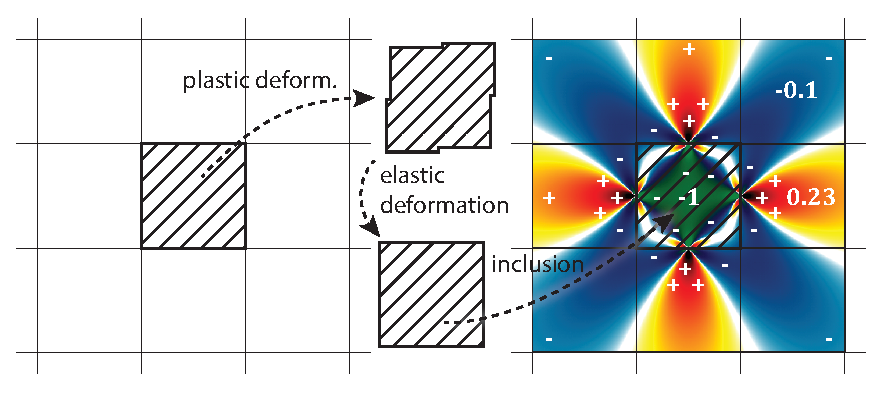
\includegraphics[width=0.6\textwidth]{arrangement}
\caption[Sketch of elementary slip event]{The sketch shows the elementary slip event. Four dislocations are placed on the edges of the active cell which causes a plastic strain $\Delta {\varepsilon ^{{\rm{pl}}}} = \Delta {\gamma ^{{\rm{pl}}}} \cdot {\bf{M}} = \Delta {\gamma ^{{\rm{pl}}}} \cdot \left( {{{\bf{e}}_x} \otimes {{\bf{e}}_y} + {{\bf{e}}_y} \otimes {{\bf{e}}_x}} \right)/2$. Then the cell is elastically deformed to fit back into its original position. The stress field this procedure generates can be calculated on the basis of the generalised Eshelby's inclusion problem and is equivalent with the stress field of the four dislocations. This deformation procedure creates the stress field shown on Fig.~\ref{fig:weakest_greens_function}. The stress field of the four dislocations are evaluated at the centerpoints of the cells.}
\label{fig:weakest_elementary_slip_event}
\end{figure}


\subsection{Discrete dislocation dynamics}
Two types of DDD models are used in this study. A time and space continuous one and one where both time and space are discretised.

\subsubsection{Time continuous DDD}
The model called time-continuous DDD (TCDDD) is the conventional DDD model, widely used in the literature. Here we consider $N$ straight parallel edge dislocations in the same slip system describing the easy slip regime of a face centered cubic (FCC) \nomenclature[z-FCC]{FCC}{face centered cubic} crystal at low temperatures (no climb and cross-slip, only glide).

There are two types of dislocations considered differing only in their Burgers vector, ${\mathbf{b}} = \left( {b,0} \right)$ and ${\mathbf{b}} = \left( {-b,0} \right)$. The first is called a positive dislocation $s=1$ and latter as a negative one $s=-1$. Equal amount of positive and negative dislocations are considered (no excess dislocations). The simulation space is square shaped with sides parallel and perpendicular to the Burgers vector and since they are edge dislocations, they move parallel to the $x$ axis, therefore only the shear component of the stress tensor plays a role in the EOM of the dislocations. An individual dislocation at the origin induce an anisotropic shear stress field at the position ${\mathbf{r}}$ as 
\begin{equation}
{\tau _{{\text{ind}}}}\left( {\mathbf{r}} \right) = x\frac{{{x^2} - {y^2}}}{{{{\left( {{x^2} + {y^2}} \right)}^2}}} = \frac{{\cos \left( \phi  \right)\cos \left( {2\phi } \right)}}{r},
\end{equation}
where $\left( {r,\phi } \right)$ are polar coordinates and units are omitted in agreement with appendix \ref{sec:dimensionless_units}.

The acting external stress is considered to be homogeneous and strong damping is considered due to phonon drag (over-damped motion) therefore the EOM of the $i$th dislocation, being at position ${{\mathbf{r}}_i} = \left( {{x_i},{y_i}} \right)$ is given by 
\begin{equation} \label{eq:weakest_EOMx}
\frac{{d{x_i}}}{{dt}} = {s_i}\left[ {{\tau _{{\text{ext}}}} + \sum\limits_{j = 1;j \ne i}^N {{s_j}{\tau _{{\text{ind}}}}\left( {{{\mathbf{r}}_i} - {{\mathbf{r}}_j}} \right)} } \right]
\end{equation}
and
\begin{equation} \label{eq:weakest_EOMy}
\frac{{d{y_i}}}{{dt}} = 0.
\end{equation}
where this latter means the absence of climb.

At the beginning of the simulations values are assigned independently to both $x$ and $y$ coordinates from a uniform distribution leading to no initial spatial correlations between the dislocations. Then \cref{eq:weakest_EOMx} is numerically solved and iterated until each dislocation reaches equilibrium defined by a low enough non-zero value limit for the average absolute velocity. This initial transient was not considered in the forthcoming evaluation as it belongs only to the generation of the initial state and time measurement is started from the end of relaxation.

In the following phase the plastic response of the system is simulated due to applied load. The external stress is increased at a constant rate till the system reaches the $v\left( t \right) > {v_{\rm{c}}}$ condition. The system is considered to be in the state of an avalanche if $v\left( t \right) > {v_{\rm{c}}}$ holds and during an avalanche the external stress is kept constant implementing a quasistatic load-controlled procedure. (The procedure is illustrated in Fig.~\ref{fig:weakest_DDD_lavina_def}.)

  
\begin{figure}[htbp!] 
\centering    
\includegraphics[width=0.6\textwidth]{bako_ddd_lavina_def}
\caption[Loading protocol and avalanches in a DDD]{On an individual realisation of a DDD simulation the quasistatic loading procedure is illustrated. If the average velocity $v$ of the dislocations (signed with their Burgers vector) is below a threshold value $v_{{\rm{c}}}$, the rate of the external stress is chosen as a constant value. If the $v>v_{{\rm{th}}}$, the external stress is kept constant.}
\label{fig:weakest_DDD_lavina_def}
\end{figure}

Plastic activity in this model has two different aspects.
\begin{enumerate}
\item During avalanches the strain rate is high and weakly depends on the external driving rate.
\item Between avalanches the strain rate is non-zero and proportional to the external stress rate and the deformation is quasireversible.
\end{enumerate}
The border of this two regimes is well defined by a carefully chosen value of ${{\dot v }_{\rm{c}}}$.

In agreement with appendix \ref{sec:dimensionless_units}, system size can be expressed by the number of dislocations as $L = {N^{0.5}}$ which explains the choice of the system sizes, chosen as $L=8,\,11.31,\,16,\,22.63,\,32$. For each system size large number of statistically equivalent realisations were taken ($3000,\,2000,\,800,\,300$ and $180$ respectively). For numerical reasons narrow enough dislocation dipoles were removed, but the introduction of this artificial length scale did not affect the phenomena investigated according to our verification.


\subsection{Cellular automaton DDD} \label{sec:weakest_CADDD}
The CADDD model is very similar to the continuous one introduced above but two restrictions are introduced which fasten up the simulation considerably.
\begin{enumerate}
\item Space is discretised into a square lattice with a cell size of $\delta$ and directions along the $x$ and $y$ axes. Dislocations can only jump from cell to a neighboring one in the $x$ direction. Only one dislocation can occupy a cell: the second dislocation of the same sign is not allowed to step to the same cell and dislocations with opposite signs annihilate each other if they are in the same cell. A very fine mesh was defined, more precisely, only every $128 \times 128$th cell was populated at the beginning.
\item Time is also discretised using the following dynamics. The acting stress $\tau$ is evaluated at both right and left edges of the cells which contain a dislocation. If the stress is positive at the right side or negative at the left side, a step towards the given direction of the stress leads to a $\Delta E \sim \;\left| \tau  \right|\delta $ decrease in the elastic energy, where $\tau$ denotes the stress at the given edge. Dislocation with such property is called active dislocation. At each time step the active dislocation with the highest possible $\Delta E$ is identified and moved by one cell in the direction determined by the largest energy drop. If none of the dislocations is active at a given time, then the external stress is increased until it is large enough to activate one, which means a quasistatic load-controlled procedure just as in the other two models.
\end{enumerate}
Like in TCDDD, simulations are started from an uncorrelated random dislocation distribution followed by an initial relaxation. The speed-up due to this technique has two main reasons.
\begin{enumerate}
\item Some details on the dynamics are erased due to the rough space and time steps.
\item The finite number of possible pair-interactions can be precalculated and stored in the memory. 
\end{enumerate}
With the introduction of this CA DDD model it becomes possible to identify the effect of the chosen dynamics -- i.e.\ extremal with CA or overdamped with continuous -- on the numerical results obtained. However, comparison is limited at the small deformation and time scales as the discrete steps corrupt the dynamics of the small avalanches and also affect the quasireversible regime observed in TCDDD, as the the motion of a dislocation either belongs to an avalanche or either is not presented at all. This is, however, not a major issue as long as macroscopic deformation, avalanche statistics and stress-strain curves are investigated.

  
\begin{figure}[htbp!] 
\centering    
\includegraphics[width=0.6\textwidth]{stress_strain_sketch}
\caption[Stress-strain curve sketch]{Sketch of the external stress-strain curves obtained from the SCPM and DDD models. The curve is made of only steps, therefore the stress and strain information on each sequence (${\tau ^{\left( i \right)}}$ and ${\gamma ^{\left( i \right)}}$, respectively) describes the whole curve.}
\label{fig:weakest_stress_strain_sketch}
\end{figure}

\section{Numerical results} \label{sec:weakest_numerical_results}
In this section the simulation results are presented and analysed for the SCPM first, and then for the two types of DDD models simultaneously. For each model the results are presented in the following order:
\begin{enumerate}
\item For each model the stress-strain curves show a step-like behaviour and differ among realisations for the same model. Therefore the average of the stress-strain curves will be in focus first.
\item Then the fluctuation in the plastic response will be evaluated.
\item Individual strain bursts are investigated then, started with the stress sequence denoted by ${\tau ^{\left( k \right)}}$. (See Fig.~\ref{fig:weakest_stress_strain_sketch} for the definition of ${\tau ^{\left( k \right)}}$.)
\item And finally the strain sequence is analysed denoted by ${\gamma ^{\left( k \right)}}$. The way the numbers are assigned and a short outlook is presented in Fig.~\ref{fig:weakest_stress_strain_sketch}.
\end{enumerate}
From now on $\tau$ will denote the external stress.

\subsection{SCPM} \label{sec:weakest_SCPM}
Three scalar parameters of the SCPM were under investigation.
\begin{enumerate}
\item The $\beta$ shape parameter of the Weibull distribution (see \cref{eq:weakest_weibull}) characterizing the local yield stress distribution.
\item The strain increment at each elementary slip deformation denoted by $\Delta {\gamma _{{\text{pl}}}}$.
\item The scale parameter $\tau_w$ characterising the average strength of a cell $\left\langle {{\tau _{{\text{th}}}}} \right\rangle $. For Weibull distributions with $\beta$ values considered in this study, ${\tau _w} \approx 1.1 \cdot \left\langle {{\tau _{{\text{th}}}}} \right\rangle $ holds.
\end{enumerate}
One of the last two parameters can be always eliminated by measuring the stress in units of $\left\langle {{\tau _{{\text{th}}}}} \right\rangle $ and strain in the units of $\Delta {\gamma _{{\text{pl}}}}$, which defines a nondimensional coupling constant $I = \Delta {\gamma _{{\text{pl}}}}/\left\langle {{\tau _{{\text{th}}}}} \right\rangle $. According to our choice $\left\langle {{\tau _{{\text{th}}}}} \right\rangle $ was set to 1 and $\Delta {\gamma _{{\text{pl}}}}$ was the variable. Where it is not stated otherwise, $\beta=1.4$ and $\Delta {\gamma _{{\text{pl}}}} = 1/4$ were used.

\subsubsection{Average stress-strain curve} \label{sec:weakest_scpm_av_ssc}


\begin{figure}[htbp] 
  \centering
  \begin{subfigure}[b]{0.44\textwidth}
    \includegraphics[width=\textwidth]{stress_strain_curve_scaled}
    \caption{The effect of the shape parameter $\beta$. The power-law region is consistent with the $\langle \tau \rangle = \gamma^{1/\beta \zeta}$ relation predicted by \cref{eq:weakest_spm_stress_expect_manyexp} with $\zeta=1$. No size effect is observed, apart from the smallest plastic regimes with large scatter in ${\tau _{{\text{th}}}}$ ($\beta=1$), the curves collapse.}
    \label{fig:weakest_avg_stress_strain_SCPM_beta}   
  \end{subfigure}                  \hspace{0.01\textwidth}
  \begin{subfigure}[b]{0.53\textwidth}
    \includegraphics[width=\textwidth]{stress_strain_scaling_SCPM}
    \caption{The effect of $\tau_w$ and $\Delta \gamma^\text{pl}$ at $\beta=1.4$ and $L=128$. According to the scaling collapse shown in the inset the average stress-strain curves obey $\langle \tau \rangle = \tau_w^{1.32} (\Delta \gamma^\text{pl})^{-0.32} f(\gamma \tau_w^{-0.5} (\Delta \gamma)^{-0.5})$ with a suitable function $f$.\\ \\}
    \label{fig:weakest_avg_stress_strain_SCPM_I}
  \end{subfigure}
  \caption[Averaged stress-strain curves for the SCPM]{The averaged stress-plastic strain curves for the SCPM. In Fig.~(a) different values for the shape parameter $\beta$, while in Fig.~(b) different $\Delta {\gamma _{{\text{pl}}}}$ were used. In each case for small strains the curves follow a power-law, then saturate.}
  \label{fig:weakest_avg_stress_strain_SCPM}
\end{figure}

The stress-strain curves of the individual realisations were averaged at given strain values. This means that at a given strain value $\gamma$ the different values of the corresponding external stress were averaged. Fig.~\ref{fig:weakest_avg_stress_strain_SCPM_beta} shows the averaged stress-strain curve for different $\beta$ values and system sizes on a double logarithmic scale. The figure shows that the microplastic regime is described by a power law, 
\begin{equation} \label{eq:weakest_SCPM_stress_strain_scale}
\left\langle \tau  \right\rangle \left( \gamma  \right) = {\tau _1}{\gamma ^\alpha }
\end{equation}
over several orders of magnitude where $\tau_1$ is a constant and the exponent $\alpha$ depends on the shape parameter $\beta$ of the Weibull distribution. The fitted values of $\alpha$ along with other scale parameters obtained from this and the other two models can be found in \cref{tab:weakest_example}. The curves show no size effect, i.e.\ for a given $\beta$ the curves for different $L$ overlap, justifying that no size scaling was introduced in \cref{eq:weakest_SCPM_stress_strain_scale}. For plastic strains $\gamma \gtrsim 1$ the stress reaches a plateau due to infinitely large avalanches signaling the onset of continuous plastic flow.

Fig.\ref{fig:weakest_avg_stress_strain_SCPM_I} shows the role of $\Delta {\gamma _{{\text{pl}}}}$ and ${\tau _w}$. It was mentioned that only $I = \Delta {\gamma _{{\text{pl}}}}/{\tau _w}$ is the independent parameter. This feature can be seen for simulations with parameters $\left( {\Delta {\gamma _{{\text{pl}}}},{\tau _w}} \right) = \left( {1/2,2} \right),$ $\left( {1,4} \right)$ and $\left( {2,8} \right)$. By dividing the plastic strain by ${\Delta {\gamma _{{\text{pl}}}}}$ and the stress by ${\tau _w}$ the curves collapse for each of the individual realisation, therefore their averaged curve too at a mathematical precision.

It can be also seen in the figure that the curve depends on the specific choice of the parameters (for different value of $I$), but according to the inset, if the stress and strains are rescaled by ${\tau _w}$ and $\Delta {\gamma _{{\text{pl}}}}$, the curves collapse into a mastercurve with a specific scaling of the parameter $I$.


\subsubsection{Fluctuations in the plastic response}


\begin{figure}[htbp!] 
  \centering
  \begin{subfigure}[b]{0.48\textwidth}
    \includegraphics[width=\textwidth]{scaled_cumulative_external_stress_probability_at_0-007813_def}
    \caption{$\gamma  = 0.008$}
    \label{fig:weakest_stress_distrib_scpma}   
  \end{subfigure}          
%  \begin{subfigure}[b]{0.48\textwidth}
%    \includegraphics[width=\textwidth]{scaled_cumulative_external_stress_probability_at_0-01563_def}
%    \caption{$\gamma  = 0.016$}
%    \label{fig:stress_distrib_scpmb}   
%  \end{subfigure}             
  \begin{subfigure}[b]{0.48\textwidth}
    \includegraphics[width=\textwidth]{scaled_cumulative_external_stress_probability_at_0-03125_def}
    \caption{$\gamma  = 0.032$}
    \label{fig:weakest_stress_distrib_scpmc}
  \end{subfigure}
  \caption[Fluctuations in the plastic response for the SCPM]{The cumulative stress distributions at different deformation values for the SCPM are shown. As system size increases the width of distributions shrink, that is, stress fluctuations disappear for large samples. By multiplying a kind of effective external stress (which can be obtained as the external stress decreased by a certain value) with a power of the system size curves can be fitted with a normal distribution (dashed line) as seen in the insets.}
  \label{fig:weakest_stress_distrib_scpm}
\end{figure}

For each of the realisations the stress-strain curve is a staircase-like function as sketched in Fig.~\ref{fig:weakest_stress_strain_sketch}, but the averaging described above makes from the ensemble of these functions a smooth one hiding the underlying details. To recover this fluctuation the cumulative distribution function (CDF) \nomenclature[z-CDF]{CDF}{cumulative distribution function} of the stresses at a given strain for different realisations is measured and denoted by ${\Phi _\gamma }\left( \tau  \right)$. The wider this curve is the larger the scatter of the external stress is which are measured for different realisations. For bulk samples the individual stress-strain curves are identical meaning that there is no fluctuation in the external stress, therefore tending to larger values with the system size one expects the width of ${\Phi _\gamma }\left( \tau  \right)$ to shrink. As seen in Fig.~\ref{fig:weakest_stress_distrib_scpm} for all strains $\gamma$ the measured ${\Phi _\gamma }\left( \tau  \right)$ curves indeed tend towards a step function as the system size increases. The stress-strain curve of a bulk material is expected to become the $\left\langle \tau  \right\rangle \left( \gamma  \right)$ curve since there is no relevant size effect observed. This also implies that the step function the ${\Phi _\gamma }\left( \tau  \right)$ CDF tends towards must be located at the given value of $\left\langle \tau  \right\rangle \left( \gamma  \right)$. It is noted that the ${\Phi _\gamma }\left( \tau  \right)$ curves for different system sizes crosses each other in the very same point. This property may hide a connection between the system parameters not revealed in this study.


All the insets in Fig.~\ref{fig:weakest_stress_distrib_scpm} show that curves collapse after scaling the stresses by the system size around $\left\langle \tau  \right\rangle \left( \gamma  \right)$. Moreover the curves (see later section \ref{sec:weakest_theory_stress_sequence} and \cref{eq:weakest_spm_stress_expect_large_i}) can be fitted by a normal distribution 
\begin{equation} \label{eq:weakest_stress_distrib}
{\Phi _\gamma }\left( \tau  \right) = \frac{1}{2}\left[ {1 + {\text{erf}}\left( {\frac{{\tau  - \left\langle \tau  \right\rangle \left( \gamma  \right)}}{{c{L^{ - \theta }}}}} \right)} \right],
\end{equation}
where $c$ is an appropriate constant and $\theta $ is the exponent characterising the system size dependence on the stress fluctuations. It was found that the no size effect can be indentified on the stress-strain curve in which case $\theta =1$ is expected. Our findings are in good agreement with this expectation as $\theta  = 1 \pm 0.05$ was found.

Previously, a shifted Weibull distribution was used to fit ${\Phi _\gamma }\left( \tau  \right)$ onto the results for 2D and 3D DDD and as well as micropillar compression data \cite{ISPANOVITY20136234}. A normal distribution, however, has fewer parameters and is in good agreement with the theoretical arguments presented later in section \ref{sec:weakest_theory_stress_sequence}.

\subsubsection{Stress sequence}

In this and the upcoming sections the stress and strain sequences ${\tau ^{\left( i \right)}}$ and ${\gamma ^{\left( i \right)}}$ will be in focus, because they play a key role in the simple plasticity model to be introduced in section \ref{sec:weakest_simple_plasticity_model}. First the cumulative distribution ${\Phi ^{\left( 1 \right)}}$ of ${\tau ^{\left( 1 \right)}}$ (the external stress at first event) will be considered. In the SCPM the plastic strain is initially homogeneous (e.g.\ zero) everywhere, therefore until the first event the local stress is also homogeneous and equal to the applied external stress everywhere according to \cref{eq:weakest_tau_loc}. As a result the distribution of the external stress at the occurance of the first plastic event must be a Weibull distribution with shape parameter $\beta$ and scale parameter ${\tau _w} \sim {L^{ - 2/\beta }}$ (for explanation see section \ref{sec:weakest_theory_stress_sequence}). According to Fig.~\ref{fig:weakest_tau_i_scpma} ${\Phi ^{\left( 1 \right)}}$ indeed follows well the corresponding Weibull distribution, and the curves for different system sizes overlap if the stress is rescaled by ${L^{2/\beta }}$.

\begin{figure}[htbp!] 
  \centering
  \begin{subfigure}[b]{0.48\textwidth}
    \includegraphics[width=\textwidth]{plotting_cumulative_prob_at_ext_stress_scaled}
    \caption{The cumulative distributions $\Phi^{(1)}$ of the first activation stress $\tau^{(1)}$ are plotted. The scaling collapse for different system sizes is obtained by rescaling the stress by $L^{2/\beta}$. The corresponding Weibull distributions (given by \cref{eq:weakest_spm_stress_cumul}) are also plotted with black lines.}
    \label{fig:weakest_tau_i_scpma}   
  \end{subfigure}          \hspace{0.01\textwidth}
  \begin{subfigure}[b]{0.48\textwidth}
    \includegraphics[width=\textwidth]{scaled_mean_stress_at_ith_avalanche_1_1_4_2}
    \caption{The average stress sequence $\langle \tau^{(i)} \rangle$ is plotted. The curves are proportional with $i^{1/\beta}$ and the ones corresponding to different system sizes collapse if stresses are rescaled by $L^{2/\beta}$, in accordance with \cref{eq:weakest_stress_sequence_average}.\\ \\}
    \label{fig:weakest_tau_i_scpmb}   
  \end{subfigure}             
  \begin{subfigure}[b]{0.46\textwidth}
    \includegraphics[width=\textwidth]{deviation_of_stress_at_ith_avalanche_1_1_4_2}
    \caption{STD of the stress sequence $\delta \tau^{(i)}$. The curves are consistent with \cref{eq:weakest_stress_sequence_std}.}
    \label{fig:weakest_tau_i_scpmc}
  \end{subfigure}
  \caption[Stress sequences for the SCPM]{The analysis of the stress sequence for different shape values $\beta=1, 1.4, 2$ and system sizes for the case of SCPM. The findings led to the simple plasticity model introduced in section \ref{sec:weakest_simple_plasticity_model}. The model prediction is plotted in each subfig with black lines.}
  \label{fig:weakest_tau_i_scpm}
\end{figure}

Fig.~\ref{fig:weakest_tau_i_scpmb} and Fig.~\ref{fig:weakest_tau_i_scpmc} plot the average stress sequence $\left\langle {{\tau ^{\left( i \right)}}} \right\rangle $ and its standard deviation (STD) \nomenclature[z-STD]{STD}{standard deviation} $\delta {\tau ^{\left( i \right)}}$, respectively. For a given shape value $\beta$ the curves collapse for small $i$ values when the stress is rescaled by ${L^{2/\beta }}$. The mastercurves follow power laws,
\begin{equation} \label{eq:weakest_stress_sequence_average}
\left\langle {{\tau ^{\left( i \right)}}} \right\rangle  = {\tau _0}{\left( {\frac{i}{{{L^\eta }}}} \right)^{1/\beta }},
\end{equation}
\begin{equation} \label{eq:weakest_stress_sequence_std}
\delta {\tau ^{\left( i \right)}} = \frac{{{\tau _0}}}{{{i^{1/2}}}}{\left( {\frac{i}{{{L^\eta }}}} \right)^{1/\beta }},
\end{equation}
where the value of $\eta $ is estimated by visual analysis and $\eta =2.0\pm0.05$ is found.



\subsubsection{Strain sequence}


\begin{figure}[htbp!] 
  \centering
  \begin{subfigure}[b]{0.48\textwidth}
    \includegraphics[width=\textwidth]{plotting_deformation_at_ith_aval_1_1_4_2}
    \caption{The averaged strain sequences can be scaled together with an appropriate transformation of the ordinate.}
    \label{fig:weakest_gamma_i_scpma}   
  \end{subfigure}           \hspace{0.01\textwidth}
  \begin{subfigure}[b]{0.48\textwidth}
    \includegraphics[width=\textwidth]{plotting_deformation_deviation_at_ith_aval_1_1_4_2}
    \caption{The STD at each index value can also scaled with the same factor as for the sequence.}
    \label{fig:weakest_gamma_i_scpmb}   
  \end{subfigure}             
  \caption[Analysis of the strain sequences for SCPM]{Strain sequences from the SCPM. The strain $\gamma^{(i)}$ measured at the $i$th strain burst for different system sizes and $\beta$ values. The curves follow \cref{eq:weakest_strain_sequence_average} and \cref{eq:weakest_strain_sequence_std} (solid lines) with $\zeta=1 \pm 0.05$ and $\xi=2 \pm 0.1$. }
  \label{fig:weakest_gamma_i_scpm}
\end{figure}


The strain sequence shows similar properties to the stress sequence. The averaged curve and its deviation can be seen in Fig.~\ref{fig:weakest_gamma_i_scpm}. For small $i$ values both $\left\langle {{\gamma ^{\left( i \right)}}} \right\rangle $ and $\delta {\gamma ^{\left( i \right)}}$ follow power laws, 
\begin{equation} \label{eq:weakest_strain_sequence_average}
\left\langle {{\gamma ^{\left( i \right)}}} \right\rangle  = {s_0}\frac{{{i^\zeta }}}{{{L^\xi }}},
\end{equation}
\begin{equation} \label{eq:weakest_strain_sequence_std}
\delta {\gamma ^{\left( i \right)}} = \frac{{{s_1}}}{{{i^{1/2}}}}\frac{{{i^\zeta }}}{{{L^\xi }}},
\end{equation}
where values for $\zeta $ and $\xi $ are obtained by visual inspections: $\zeta  = 1.0 \pm 0.05$ and $\xi  = 2.0 \pm 0.1$. We found that both $\zeta $ and $\xi $ are insensitive to the exponent $\beta$ but ${{\gamma ^{\left( i \right)}}}$ and $\delta {\gamma ^{\left( i \right)}}$ themselves are sensitive, therefore $s_0$ and $s_1$ too. It means that the size of individual avalanches vary significantly in different cases.


\subsection{DDD models}
\subsubsection{Average stress-strain curve}

The average stress-strain curves for the DDD models were calculated the same way as for the SCPM detailed in section \ref{sec:weakest_scpm_av_ssc}. The stress-strain curves can be seen in Fig.~\ref{fig:weakest_avg_stress_strain_DDD} which show similar features to those obtained by the SCPM case, namely:
\begin{enumerate}
\item The microplastic regime is characterised by a power law with an exponent $\alpha  = 0.8 \pm 0.05$ (see \cref{eq:weakest_SCPM_stress_strain_scale}) and only a weak size effect can be seen.
\item This regime breaks down at $\tau  \approx 0.1$.
\item The curves saturate for large ($\gamma \gtrsim 10$) strains.
\end{enumerate}

\begin{figure}[htbp!] 
  \centering
  \begin{subfigure}[b]{0.48\textwidth}
    \includegraphics[width=\textwidth]{stress-average-at-gamma_v2}
    \caption{TCDDD}
    \label{fig:weakest_avg_stress_strain_TCDDD}   
  \end{subfigure}          
  \begin{subfigure}[b]{0.48\textwidth}
    \includegraphics[width=\textwidth]{avg_stress_strain_ca}
    \caption{CADDD}
    \label{fig:weakest_avg_stress_strain_CADDD}   
  \end{subfigure}             
  \caption[Analysis of the stress sequence for DDDs]{The average stress-strain curves of the DDD simulations. They follow a power-law until $\gamma \approx 0.1$, and saturate for large ($\gamma \gtrsim 10$) strains.}
  \label{fig:weakest_avg_stress_strain_DDD}
\end{figure}


Significant difference in the averaged stress-strain curves between the two DDD models arises only at large strains. In the work of \citet{1742-5468-2015-8-P08009} it is discussed, that the source of this discrepancy can be originated from artifact of the periodic boundary conditions. This phenomenon does not play any role at the initial part of the stress-strain curve, therefore it does not affect the statistical arguments presented in the followings, which is valid for small to medium strains only where the two DDD models exhibit similar behaviour.




\subsubsection{Fluctuation in the plastic response}

\begin{figure}[htbp!] 
  \centering
  \begin{subfigure}[b]{0.48\textwidth}
    \includegraphics[width=\textwidth]{TCDDD_stress-distrib-0_05}
    \caption{TCDDD; $\gamma = 0.05$}
    \label{fig:weakest_stress_distrib_ddd_TCDDD_005}   
  \end{subfigure}          
  \begin{subfigure}[b]{0.48\textwidth}
    \includegraphics[width=\textwidth]{TCDDD_stress-distrib-0_2}
    \caption{TCDDD; $\gamma = 0.2$}
    \label{fig:weakest_stress_distrib_ddd_TCDDD_02}   
  \end{subfigure}             
  \begin{subfigure}[b]{0.48\textwidth}
    \includegraphics[width=\textwidth]{CADDD_stress-distrib-0_05}
    \caption{CADDD; $\gamma = 0.05$}
    \label{fig:weakest_stress_distrib_ddd_CADDD_005}   
  \end{subfigure}          
  \begin{subfigure}[b]{0.48\textwidth}
    \includegraphics[width=\textwidth]{CADDD_stress-distrib-0_2}
    \caption{CADDD; $\gamma = 0.2$}
    \label{fig:weakest_stress_distrib_ddd_CADDD_02}   
  \end{subfigure}             
  \caption[Stress sequences for the DDDs]{The cumulative stress distributions $\Phi_\gamma$ at two different deformation levels $\gamma$ for the two DDD models. Scaling collapse can be obtained (see insets) by multiplying a kind of effective external stress (obtained by subtracting a certain value from the external stress) with a power of the system size, just as for the SCPM in Fig.~\ref{fig:weakest_stress_distrib_scpm}. The collapsed curves can be well fitted by an appropriate normal distribution (dashed lines).}
  \label{fig:weakest_stress_distrib_ddd}
\end{figure}



In Fig.~\ref{fig:weakest_stress_distrib_ddd} cumulative distributions ${\Phi _\gamma }\left( \tau  \right)$ of the stresses for different realisations at a given strain $\gamma$ are calculated and plotted, just as for the SCPM case, and the curves also share the similarities. Namely, the curves
\begin{enumerate}
\item tend to step functions as the system size increases,
\item intersect in a single point,
\item can be collapsed by scaling the stress with a certain power of the system size,
\item are well approximated by a normal distribution.
\end{enumerate}
As a consequence of the last point, \cref{eq:weakest_stress_distrib} holds with the proper exponent, here $\theta  = 0.8 \pm 0.05$, which means the system shows size dependency in this sense. Note that $0.8 = {\theta _{{\text{DDD}}}} < {\theta _{{\text{SCPM}}}} = 1$.




\subsubsection{The stress sequence}
\begin{figure}[htbp!] 
  \centering
  \begin{subfigure}[b]{0.48\textwidth}
    \includegraphics[width=\textwidth]{first-aval-stress_v3}
    \caption{The cumulative distribution $\Phi^{(1)}$ of the first activation stress $\tau^{(1)}$. Data collapse is obtained by plotting $\Phi^{(1)}$ as a function of $\tau L^{1.15}$ in the inset, plotted along a Weibull distribution with $\beta \approx 1.4 \pm 0.05$.}
    \label{fig:weakest_tau_i_tacdda}   
  \end{subfigure}           \hspace{0.01\textwidth}
  \begin{subfigure}[b]{0.48\textwidth} 
    \includegraphics[width=\textwidth]{i-th-aval-mean-stress}
    \caption{The average of the external stress $\tau^{(i)}$ at the \textit{i}th avalanche for different system sizes. The data are consistent with \cref{eq:weakest_stress_sequence_average} (solid lines) if $i\gtrsim3$ and $\langle \tau^{(i)}\rangle \lesssim 0.2$ and with $\beta = 1.4 \pm 0.05$ and $\eta = 1.6 \pm 0.1$.}
    \label{fig:weakest_tau_i_tacddb}   
  \end{subfigure}             
  \begin{subfigure}[b]{0.48\textwidth}
    \includegraphics[width=\textwidth]{i-th-aval-deviation-stress}
    \caption{The STD of the external stress $\tau^{(i)}$ at the \textit{i}th avalanche for different system sizes. The data are consistent with \cref{eq:weakest_stress_sequence_std} (solid lines) if $i\gtrsim3$ and $\langle \tau^{(i)}\rangle \lesssim 0.2$ and with $\beta = 1.4 \pm 0.05$ and $\eta = 1.6 \pm 0.1$.}
    \label{fig:weakest_tau_i_tacddc}
  \end{subfigure}
  \caption[Stress sequences for the TCDDD]{The analysis of the stress sequence $\tau^{(i)}$ for TCDDD simulations of different system sizes. Predictions according to the simple plasticity model introduced in \ref{sec:weakest_simple_plasticity_model} is plotted with black lines.}
  \label{fig:weakest_tau_i_tacdd}
\end{figure}


As mentioned in the description of the CADDD model \ref{sec:weakest_CADDD}, inter-avalanche events cannot be distinguished from small avalanches, therefore they ruin the statistics in investigating the stress and strain sequence at the low strain/stress limit. As a consequence, only the TCDDD model will be used in this analysis.

For the CADDD case, the analysis of the stress sequence can be seen in Fig.~\ref{fig:weakest_tau_i_tacdd}. According to Fig.~\ref{fig:weakest_tau_i_tacdda}, where the cumulative distribution ${\Phi ^{\left( 1 \right)}}$ of ${\tau ^{\left( 1 \right)}}$ (the external stress at the first plastic event) is plotted, a Weibull distribution with the proper shape parameter $\beta$ can be perfectly fitted onto the curve after collapsing the curves into a mastercurve (shown in the inset) via rescaling ${\tau ^{\left( 1 \right)}}$ by ${L^{\eta /\beta }}$ with parameters
\begin{equation} \label{eq:weakest_tcddd_beta}
  \beta  =  1.4 \pm 0.05,
\end{equation}
\begin{equation} \label{eq:weakest_tcddd_eta}
  \eta  =  1.6 \pm 0.1. 
\end{equation}

The rescaled $\left\langle {{\tau ^{\left( i \right)}}} \right\rangle $ and $\delta {\tau ^{\left( i \right)}}$ obey the same rule observed for SCPM in  \cref{eq:weakest_stress_sequence_average,eq:weakest_stress_sequence_std} and share the parameters as in \cref{eq:weakest_tcddd_beta,eq:weakest_tcddd_eta}.



\subsubsection{Strain sequence}

Figure \ref{fig:weakest_gamma_i_CADDD} shows some statistics on the strain measured at the $i$th event. The average strain $\left\langle {{\gamma ^{\left( i \right)}}} \right\rangle $ at the burst of the $i$th avalanche can be seen in Fig.~\ref{fig:weakest_gamma_i_CADDDa} and its STD in Fig.~\ref{fig:weakest_gamma_i_CADDDb}. The curves are in good agreement with \cref{eq:weakest_strain_sequence_average,eq:weakest_strain_sequence_std} estabilished for the SCPM first, but here the exponents were $\zeta  = 0.9 \pm 0.05$ and $\xi  = 1.5 \pm 0.1$.


\begin{figure}[htbp!] 
  \centering
  \begin{subfigure}[b]{0.48\textwidth}
    \includegraphics[width=\textwidth]{plotting_deformation_at_ith_aval_1_1_4_2}
    \caption{The averaged strain sequences can be scaled together with an appropriate transformation of the ordinate.}
    \label{fig:weakest_gamma_i_CADDDa}   
  \end{subfigure}           \hspace{0.01\textwidth}
  \begin{subfigure}[b]{0.48\textwidth}
    \includegraphics[width=\textwidth]{plotting_deformation_deviation_at_ith_aval_1_1_4_2}
    \caption{The STD at each index value can also scaled with the same factor as that of the sequence.}
    \label{fig:weakest_gamma_i_CADDDb}   
  \end{subfigure}             
  \caption[Analysis of the strain sequences for SCPM]{Strain sequences from the TCDDD. The strain $\gamma^{(i)}$ measured at the $i$th strain burst for different system sizes and $\beta$ values. The curves follow \cref{eq:weakest_strain_sequence_average}) and \cref{eq:weakest_strain_sequence_std} (solid lines) with $\zeta=0.9 \pm 0.05$ and $\xi=1.5 \pm 0.1$ for large enough system sizes. }
  \label{fig:weakest_gamma_i_CADDD}
\end{figure}


A summary of all the exponents introduced in this section can be found in Table~\ref{tab:weakest_example}.

\section{Simple plasticity model based on order statistics} \label{sec:weakest_simple_plasticity_model}

A simple plasticity model is introduced in this section based on the numerical results obtained in the previous sections of this chapter. In this model the deformation is stress controlled, elastic deformation is neglected and the stress-strain curve is a monotonous staircase function, which is completely characterised by the stress-strain sequence $\left( {{\tau ^{\left( i \right)}},{\gamma ^{\left( i \right)}}} \right)$ (for a sketch see \ref{fig:weakest_stress_strain_sketch}). The intention behind this picture is to model the stochastic feature of the plasticity investigated numerically in the previous section, therefore scaling forms in the model proposed will share the same notations as used at the evaluation of the results. A comprehensive overviewof the parameters can be found in Table.~\ref{tab:weakest_example}.

In this model we adopt the work of \citet{doi:10.1080/14786435.2014.932502} using a weakest link assumption to express the mean value of the stress sequence ${\tau ^{\left( i \right)}}$ and its STD. From the work of \citet{PhysRevLett.112.235501} we adopt a straightforward rule for the strain sequence to obtain the mean value and STD of the strain sequence in the TCDDD model too, where anomalous system size scaling has been observed. The combination of the stress and strain sequences gives a statistical prediction on the stress-strain curve which affirm our numerical results in section \ref{sec:weakest_numerical_results}. In our model the material can be decomposed into smaller units which interact via only the stress-field kernel. In the small deformation limit the plastic events are localised into a smaller portion of the material and the starting points of the avalanches are not affected by the deformation history.

In this model we will further assume, that
\begin{enumerate}
\item The Weibull-shaped activation threshold of a plastic events remains unchanged during plastic deformation.
\item The distribution of the avalanche size is stress independent.
\item By splitting up the stress-strain curve into small segments, in each interval many avalanches occur so that the summation of the strain sequences leads to a normal distribution according to the central limit theorem.
\end{enumerate}
The validity of the first two is questionable in a general case, especially for the SCPM where critical behaviour at high enough external stress can be observed, but can be accepted at the limit of small stresses, where avalanches are rather localised and not limited by the system size. The third assumption can be always legitimated if the system size $L$ is large enough.


\subsection{Stress sequence}  \label{sec:weakest_theory_stress_sequence}
The main idea of the SCPM is that plasticity occurs via irreversible local structural excitations which are activated at different stress values. This critical stress distribution $P\left( \tau  \right) = \frac{d}{{d\tau }}\Phi \left( \tau  \right)$ (the derivative of the cumulative distribution) represents the inhomogenities in the material at the resolution of the mesh size. During the stress increase the weakest sites are activated first, therefore only the $\tau  \to 0$ limit of this distribution plays a role at low strains. A reasonable proposition for this distribution \cite{doi:10.1080/14786435.2014.932502} is a power law as
\begin{equation} \label{eq:weakest_cumulative_is_power_law}
\Phi \left( \tau  \right) = {\left( {\frac{\tau }{{{\tau _0}}}} \right)^\beta }\quad {\text{if }}\tau  \to 0
\end{equation}
with $\beta \geqslant 1$. It is also assumed that the subsequent events are independent, i.e.\ no spatial correlations in the stress and plastic strain is present initially (at the low strain limit). If the number of independent sites is $M$, and $M \to \infty$, then the cumulative distribution of the $i$th stress value ${\tau ^{\left( i \right)}}$ follows a Weibull order statistics \cite{rinne2008weibull}, e.g.\ for the first value it is
\begin{equation} \label{eq:weakest_spm_stress_cumul}
{\Phi ^{\left( {1,M} \right)}}\left( {{\tau ^{\left( {1,M} \right)}}} \right) = 1 - \exp \left[ { - \frac{1}{M}{{\left( {\frac{{{\tau ^{\left( {1,M} \right)}}}}{{{\tau _0}}}} \right)}^\beta }} \right].
\end{equation}
The expected value of the $i$th event is given by
\begin{equation}  \label{eq:weakest_spm_stress_expect}
\left\langle {{\tau ^{\left( {i,M} \right)}}} \right\rangle  = \frac{{{\tau _0}}}{{{M^{1/\beta }}}}\frac{{\Gamma \left( {i + 1/\beta } \right)}}{{\Gamma \left( i \right)}} \approx {\tau _0}{\left( {\frac{i}{M}} \right)^{1/\beta }},
\end{equation}
and the STD by
\begin{equation}  \label{eq:weakest_spm_stress_deviat}
\delta {\tau ^{\left( {i,M} \right)}} = \sqrt {{{\left( {\frac{{{\tau _0}}}{{{M^{1/\beta }}}}} \right)}^2}\frac{{\Gamma \left( {i + 2/\beta } \right)}}{{\Gamma \left( i \right)}} - {{\left( {\frac{{\Gamma \left( {i + 1/\beta } \right)}}{{\Gamma \left( i \right)}}} \right)}^2}}  \approx \frac{{{\tau _0}}}{{{i^{1/2}}}}{\left( {\frac{i}{M}} \right)^{1/\beta }},
\end{equation}
where the approximation is exact in the limit when $i \to \infty$, $M \to \infty$ and $i/M \to 0$, and the error is less than $2\%$ if $i>5$ and if $M > 1000 \cdot i$ \citep[Sec. 6.1.47.]{abramowitz1964handbook}.

The findings are not restricted to only to the first few plastic events, but also applicable in the regime of order statistics, where $i/M=p$ finite. In the asymptotic limit, when $M \to \infty$ and $i/M=p$ is finite, the probability density function (PDF) \nomenclature[z-PDF]{PDF}{probability density function} of the $i$th smallest member drawn from $M$ samples -- whose CDF is $\Phi \left( \tau  \right)$ -- is normal distributed according to the central limit theorem, and its CDF is
\begin{equation} \label{eq:weakest_spm_stress_expect_large_i}
{\Phi ^{\left( {i,M} \right)}}\left( {{\tau ^{\left( {i,M} \right)}}} \right) = \frac{1}{2}\left[ {1 + {\text{erf}}\left( {\frac{{{\tau ^{\left( {i,M} \right)}} - \left\langle {{\tau ^{\left( {i,M} \right)}}} \right\rangle }}{{{\sigma ^{\left( {i,M} \right)}}}}} \right)} \right],
\end{equation}
in which the expected value is given by \cite{dasgupta2008asymptotic}
\begin{equation}
\left\langle {{\tau ^{\left( {i,M} \right)}}} \right\rangle  = {\Phi ^{ - 1}}\left( p \right): = \tau \left( p \right),
\end{equation}
and the deviation by
\begin{equation}
{\sigma ^{\left( {i,M} \right)}} = {\left( {\frac{{p\left( {1 - p} \right)}}{{M \cdot {{\left[ {\Phi '\left( {\tau \left( p \right)} \right)} \right]}^2}}}} \right)^{1/2}},
\end{equation}
where ${\Phi ^{ - 1}}\left( p \right)$ is the inverse of the CDF $\Phi \left( \tau \right)$ and $\Phi '$ is the derivative of the CDF, $\Phi ' = \frac{d}{{d\tau }}\Phi \left( \tau  \right)$. It was found that for small $p$ the CDF is $\Phi  \approx {\left( {\tau /{\tau _w}} \right)^\beta }$ which recovers \cref{eq:weakest_spm_stress_expect,eq:weakest_spm_stress_deviat}, hence extreme order statistics is applicable in the regime of finite $i/M$ too.

The connection between the number of sites $M$ and linear system size $L$ can be also discussed in the framework of this simple plasticity model. According to a common assumption, all sites are homogeneously distributed where plastic event can occur and their density does not depend on the system size. This leads to a $M \propto {L^d}$ connection, where $d$ is the physical dimension of  the system, in our case, $d=2$. In the DDD case results have shown anomalous size dependence which requires the refinement of this connection. Instead of $d$, a fractal dimension $\eta$ is introduced to describe the size dependence in the form
\begin{equation} \label{eq:weakest_anomalous_link_scaling}
M \propto L^\eta.
\end{equation}
Substituting this \cref{eq:weakest_anomalous_link_scaling} into \cref{eq:weakest_spm_stress_cumul,eq:weakest_spm_stress_expect,eq:weakest_spm_stress_deviat}, one gets
\begin{equation}
{\Phi ^{\left( 1 \right)}}\left( {{\tau ^{\left( 1 \right)}}} \right) =  1 - \exp \left( { - {{\left[ {\frac{1}{{{\tau _0}}}\frac{{{\tau ^{\left( 1 \right)}}}}{{{L^{\eta /\beta }}}}} \right]}^\beta }} \right),
\end{equation}
\begin{equation}
{\tau ^{\left( i \right)}} \approx  {\tau _0}{L^{ - \eta /\beta }} \cdot {i^{1/\beta }},
\end{equation}
and
\begin{equation}
\delta {\tau ^{\left( i \right)}} \approx  {L^{ - \eta /\beta }} \cdot {i^{1/\beta  - 1/2}}.
\end{equation}


\begin{table}[htpb]
\newcolumntype{L}[1]{>{\raggedright\let\newline\\\arraybackslash\hspace{0pt}}m{#1}}
\newcolumntype{C}[1]{>{\centering\let\newline\\\arraybackslash\hspace{0pt}}m{#1}}
\newcolumntype{R}[1]{>{\raggedleft\let\newline\\\arraybackslash\hspace{0pt}}m{#1}}
\centering
\caption{Summary of the exponents used in this study.}
\label{tab:weakest_example}
\begin{tabular}{L{1cm} L{4.0cm} C{2.1cm} C{1.7cm} C{2.0cm} C{2.0cm}}
\hline
Symbol & Description & Value predicted by theory & Value for SCPM & Value for TCDDD & Value for CADDD \\
\hline
$\beta$ & Characterizes threshold stress distribution, see \cref{eq:weakest_cumulative_is_power_law})  & - & $1.0$, $1.4$, and $2.0$\tablefootnote{This exponent is an input parameter for the SCPM model} & $1.4 \pm 0.05$ & - \\
$\eta$ & Describes the relation between the system size $L$ and the total number of links $M$, see \cref{eq:weakest_anomalous_link_scaling}) & - & $2.0 \pm 0.05$ & $1.6 \pm 0.1$ & - \\
$\zeta$ & Characterizes the strain sequence, see \cref{eq:weakest_spm_strain_expect}) & - & $1.0 \pm 0.05$ & $0.9 \pm 0.05$ & - \\
$\xi$ & Characterizes the system size dependence of the average avalanche size, see \cref{eq:weakest_gamma_step_average}) & $\eta \zeta$ & $2.0 \pm 0.1$ & $1.5 \pm 0.1$ & - \\
$\alpha$ & Exponent of the power-law characterizing the microplastic regime of the stress-strain curves, see \cref{eq:weakest_SCPM_stress_strain_scale}& $(\beta \zeta)^{-1}$ & $1.0\pm 0.05$, $0.7\pm 0.05$, and $0.5 \pm 0.05$ & $0.8\pm 0.05$ & $0.8 \pm 0.05$\\
$\theta$ & Exponent characterizing the system size dependence of the stress fluctuations, see \cref{eq:weakest_stress_distrib}) & $\eta/2$ & $1.0 \pm 0.05$ &  $0.8 \pm 0.05$ & $0.8 \pm 0.05$ \\
\end{tabular}
\end{table}

\subsection{Strain sequence}
The size of strain burst events may exhibit power-law distribution, revealed by recent experimental and numerical studies \cite{Dimiduk1188,doi:10.1080/14786430802132522,PhysRevLett.112.235501,miguel2001intermittent}. This distribution $P\left( {\Delta \gamma } \right)$ is upper bounded by ${\Delta {\gamma _u}}$, which can originate from the system size or other intrinsic bounds inherent in dynamics, and lower bounded by $\Delta {\gamma _l}$ due to the fact that a power law distribution with exponent smaller than $-1$ cannot be normalised around the singularity at 0. This boundary can be originated from e.g.\ the mean dislocation spacing -- which is orders of magnitude larger than the size of the dislocation core --, below which the individual dislocation motion may be the major source of plastic strain. Restricting our model above the lower  boundary, the size distribution can be written as
\begin{equation}
P\left( {\Delta \gamma } \right) = C \cdot \Delta {\gamma ^{ - {\tau _a}}} \cdot f\left( {\Delta \gamma /\Delta {\gamma _u}} \right)\quad {\text{if }}\Delta \gamma  > \Delta {\gamma _l}
\end{equation}
where ${\Delta \gamma }$ is the size of the strain increment, $C$ is a normalisation factor, ${{\tau _a}}$ is the avalanche size exponent and $f\left( x \right)$ is a cutoff function, which tends to $1$ for $x \to 0$ , and tends to $0$ for $x \to \infty$.

According to the work of \citet{PhysRevLett.112.235501}, $\tau^a \approx 1$ was found in the microplastic regime and $\Delta \gamma_u$ depends only weakly on the allied stress and exhibits anomalous system size dependence. In a work of \citet{1742-5468-2015-2-P02011}, for the SCPM case, $\tau_a \approx 1.35$ was found, and $\Delta \gamma_u$ diverges at a critical stress and exhibits regular system size dependence. The mean value of the strain size and its variance can be written in both cases as 
\begin{equation} \label{eq:weakest_gamma_step_average}
\left\langle {\Delta \gamma } \right\rangle  = \frac{{{s_0}}}{{{L^\xi }}},
\end{equation}
\begin{equation}  \label{eq:weakest_gamma_step_deviat}
\delta \left( {\Delta \gamma } \right) = \frac{{{s_1}}}{{{L^\xi }}},
\end{equation}
where $\xi$ is the exponent characterising the system size dependence, and $s_0$ and $s_1$ are constants depending e.g.\ on the applied stress. For the 2D DDD case, $\xi < 2$ represents anomalous scaling, where the total size of a plastic event depends on the system size. Value $\xi = 2$ correspond to normal scaling in 2D, as it was found for the SCPM.

In case one can assume the independence of the size of the subsequent events, central limit theorem for large enough $i$ values gives the value of the mean and variance in the form of 
\begin{equation} \label{eq:weakest_spm_strain_expect}
\left\langle {{\gamma ^{\left( i \right)}}} \right\rangle  = {i^\zeta }\left\langle {\Delta \gamma } \right\rangle  = {i^\zeta }\frac{{{s_0}}}{{{L^\xi }}}
\end{equation}
and
\begin{equation} \label{eq:weakest_spm_strain_deviat}
\delta {\gamma ^{\left( i \right)}} = {i^{\zeta  - 1/2}}\delta \left( {\Delta \gamma } \right) = \frac{{{i^\zeta }}}{{{i^{1/2}}}}\frac{{{s_1}}}{{{L^\xi }}}.
\end{equation}

\subsection{Stress-strain curves}
The possibility to express the stress-strain curve for one realisation from the individual ${\tau ^{\left( i \right)}}$ and ${\gamma ^{\left( i \right)}}$ sequences is given as they completely characterise the curve. For a given large enough value $i$ both follow a normal distribution according to \cref{eq:weakest_spm_stress_expect,eq:weakest_spm_stress_deviat} and to \cref{eq:weakest_spm_strain_expect,eq:weakest_spm_strain_deviat}. By inverting $\left\langle {{\gamma ^{\left( i \right)}}} \right\rangle \left( i \right)$ and substitute the value $i$ into ${\tau ^{\left( i \right)}}$ and using the approximation 
\begin{equation}
\left\langle {{\tau ^{\left( i \right)}}} \right\rangle \left( \gamma  \right) \approx {\tau ^{\left( {{{\left\langle {{\gamma ^{\left( i \right)}}} \right\rangle }^{ - 1}}\left( \gamma  \right)} \right)}},
\end{equation}
one gets 
\begin{equation} \label{eq:weakest_spm_stress_expect_manyexp}
\left\langle \tau  \right\rangle \left( \gamma  \right) = \frac{{{\tau _0}}}{{s_0^{1/\left( {\beta \zeta } \right)}}}{L^{\left( {\xi /\zeta  - \eta } \right)/\beta }}{\gamma ^{1/\beta \zeta }}
\end{equation}
and 
\begin{equation} \label{eq:weakest_spm_stress_deviat_manyexp}
\delta \tau \left( \gamma  \right) = {\tau _2}{L^{\left( {\xi /\zeta  - \eta } \right)/\beta  - \xi /\left( {2\zeta } \right)}} \cdot {\gamma ^{\left( {1/\beta  - 1/2} \right)/\zeta }}
\end{equation}
with ${\tau _2} = {\tau _0}/s_0^{\left( {1/\beta  - 1/2} \right)/\zeta }$. In this approximation the stress-strain curve follows power law and has a system size dependence for all (large) $L$ values if $\left( {\xi /\zeta  - \eta } \right)/\beta  \ne 0$. To avoid this non-physical behaviour, 
\begin{equation}
\xi  = \zeta \eta
\end{equation}
must hold. In this case \cref{eq:weakest_spm_stress_expect_manyexp,eq:weakest_spm_stress_deviat_manyexp} have the form
\begin{equation}
\left\langle \tau  \right\rangle \left( \gamma  \right) \propto {\gamma ^\alpha }\quad \alpha  = 1/\beta \zeta 
\end{equation}
and
\begin{equation} \label{eq:weakest_spm_stress_deviat_oneexp}
\delta \tau \left( \gamma  \right) \propto {L^{ - \theta }}\quad \theta  = \eta /2.
\end{equation}
\Cref{eq:weakest_spm_stress_deviat_oneexp} says that with increasing system size the STD decreases since $\theta>0$ and one obtains a well-defined, system size independent curve in the $L \to \infty$ limit.

\section{Summary}
The main idea of our SCPM is that a crystalline material can be treated as an arrangement of independent smaller units, each characterised by a local flow threshold (i.e.\ activation stress of a local plastic strain event) accounting for the inhomogeneity of the underlying dislocation microstructure not taken into account completely on the continuum level. According to the weakest link theory, the PDF of the external stress ${\tau ^{\left( 1 \right)}}$ at the onset of the first activated plastic event must follow a Weibull distribution.

This idea was supported by the numerical results of the TCDDD model, where the PDF of ${\tau ^{\left( 1 \right)}}$ followed a Weibull distribution with a shape parameter $\beta$ independent from the system size. Moreover, the shape parameter not only determines the asymptotic behaviour of the PDF of the stress threshold for the individual units, which is a power low with an exponent of $\beta$, but also plays a central role in forming the stress-strain curve. Theoretical explanation of the value found for $\beta \approx 1.4$ is out of the scope of this study, but similar connection can be found in 3D DDD models and in micropillar compression tests too \cite{ispanovity2010submicron,ISPANOVITY20136234}, where the stress-strain curves are investigated and obtained that $\alpha  = 1/\left( {\beta \zeta } \right) = 0.8$. In the following chapter (chapter \ref{chapter:disorder})) the role of $\beta$ in ductility of disordered materials exhibiting strain softening will be presented.

For both the SCPM and the DDD models the stress sequence followed a power law, with and exponent $\eta$ characterising the system size dependence. For the case of SCPM $\eta \approx 2$ was found representing normal system size scaling, i.e.\ the number of sites $M$ which can be activated scales with the linear size of the system on the power of the system dimension, $M \propto L^2$. Whereas for DDD $\eta \approx 1.5$ was found, a significantly smaller number than the physical dimension of the system suggesting a fractal-like arrangement of the activated sites. This presumption can be checked by calculating the correlation integral $C\left( r \right)$ for the coordinates\footnote{The correlation integral $C\left( r \right)$ on a set of points gives the frequency that two points can be found within a smaller distance than $r$.} of the dislocation avalanches.\footnote{By the coordinates of an avalanche we took the coordinates of the first plastic event within the avalanche.} Figure~\ref{fig:corrlation_integral} shows this correlation integral for the SCPM and DDD model. It tells that for large enough $r$ values they can be approximated by a power law and the findings support our conjecture: for the SCPM case the place of plastic strains follows a $r^2$ dependence while for the DDD case the function goes as $r^{1.6}$, i.e.\ the plastic strains are indeed accumulated on a fractal pattern of the material. This is in good agreement with the work of \citet{weiss2003three}, which states that the sources of the accousic emission signals are located on a fractal layer, morever, the fractal behaviour in our DDD model could explain the long-range nature of the correlations observed in the work of \citet{PhysRevLett.112.235501} investigating 2D DDD system, however, the origin of this fractal phenomenon is out of the scope of this study.


\begin{figure}[htbp!] 
\centering    
\includegraphics[width=0.6\textwidth]{corr_int}
\caption[Coreelation integral]{The correlation integrals of the starting positions of the avalanches for the SCPM and TCDDD models are plotted on a log-log scale. For both cases the integral follows a power law $C\left( r \right) \propto {r^\eta }$, with $\eta \approx 2.0$ and $\eta \approx 1.6$, respectively. Power laws with these exponents are also plotted with solid black lines.}
\label{fig:corrlation_integral}
\end{figure}

It is important to note that the size effects found in this study are not in connection with those general phenomena observed in other samples, where size effects come from surface effects as dislocation pile ups or dislocations running out of the sample at free boundary, but represents the behaviour of bulk samples as we implemented periodic boundary conditions. This boundary condition may lead to nonphysical artifacts (e.g.\ Fig.~\ref{fig:weakest_avg_stress_strain_CADDD} shows inverse size effect for large strains) which can be handled with an appropriate modification of the boundary conditions \cite{1742-5468-2015-8-P08009}.

The theoretical models used in this study are capable of describing the microplastic regime of micron-scale samples. We also found that there are only two independent exponents, $\beta$ and $\eta$, which, on the one hand, represent microstructural details of the material, on the other hand, they are directly linked to macroscopic quantities. $\beta$ can be obtained from the microplastic regime of stress-strain curve identifying the exponent of the power law, while $\eta$ can be determined from the stress fluctuations of different samples. By measuring these parameters in a model or even in real experiments one can set up the SCPM to reflect the desired behaviour . Figure~\ref{fig:stress_strain_comparison} shows a well configured SCPM in order to give similar results at microplastic regime then what we got for the DDD models. The fact that the stress-strain curve of the SCPM follows well the curve obtained for DDD models at larger strains too does not necessarily hold relevance as the model doesn't capture the internal strain correlations observed in DDD models.

\begin{figure}[htbp!] 
\centering    
\includegraphics[width=0.6\textwidth]{stress_strain_comparison}
\caption[Stress-strain curve comparison]{The stress-strain curves obtained from the three different plasticity models. The parameters of the SCPM were: $\beta  = 1.4$, $\Delta {\gamma _{{\rm{pl}}}} = 6$ and ${\tau _w} = 2$.}
\label{fig:stress_strain_comparison}
\end{figure}

\section*{Notes in regard to the thesis}
In this study we demonstrated that the SCPM model introduced earlier is capable of describing the stochastic properties of materials in the microplastic regime. A simple plasticity model has been proposed which is founded on the subsequent plastic events of crystalline samples in the microplastic regime. A methodology was proposed to compare the results of the SCPM and DDD models, which is suitable to determine how the free parameters of the SCPM should be chosen in order to reproduce the behaviour observed in the lower level DDD simulations.

The SCPM introduced earlier is based on a continuum model using the self-consistent field approximation which neglects the initial correlations of dislocations and let them evolve only through the signed (excess) dislocation density. It is known that such system exhibit non physical behaviour, e.g.\ the energy of the dislocation system is not an extensive quantity. However, this model is still suitable to describe some properties of the stochastic phenomena observed in crystal plasticity and gives an idea how to handle correctly the appearing $C$ parameter occurring in the local flow stress introduced in the continuum model with local density approximation at \cref{eq:flow_stress}.

My specific contribution to this study was primarily based on the SCPM. Based on the description found in the work of \citet{1742-5468-2005-08-P08004} I implemented a model first which reproduces the same statistics. Our target was to run large number of simulations but due to our moderate computational resources an efficient and free software was needed. Therefore, I wrote the whole program in C++. I further extended the model with the possibility to chose a local flowstress distribution, the actual form of the interaction kernel $G_E$ and the size of the plastic event along some other details not mentioned so far. I performed all the analysis of the data and contributed in preparing the corresponding manuscript and in preparing the figures therein.

It was also mentioned that the validity of this SCPM is not restricted to crystalline materials only but can be also used in amorphous materials. A model essentially based on this implementation can be found in the next chapter \ref{chapter:disorder}.

\subsection*{Negative results}

The reason why many other parameters or details have been investigated lies in our initial goal, which was namely to investigate the size distribution of the avalanches and how the parameters of the SCPM modify it. I also tried to point out the non-depinning behaviour of dislocation avalanches with the SCPM developed but it turned out that either the size scale used is too small to verify our goal or this is not the case, i.e.\ dislocations/dislocation groups are pinned at each site and a critical stress (yield stress) indeed exists where infinite large event occurs. It was also desired to find an anomalous system size scaling but our efforts rewarded no success and to exclude the possibility, that it is due to the small system size, large system sizes were again desirable. To achieve larger system sizes than $512 \times 512$, a program code for GPU has been written in CUDA which gave the same results as the one written in C++ and due to the nature of GPGPU the simulation time scales favourably with the system size and already at the size of $1024 \times 1024$ runs faster then on CPU\footnote{performed on an architecture which costs the same amount of money}. Unfortunately the acquisition of such devices has been canceled and only further improvements in the CPU code moved forward the investigation of the influence of the system size. The sophisticated CPU code on larger systems still didn't produce the results desired which made me to focus on other properties of the model, i.e.\ how to correctly set up all the parameters introduced in this model instead of their effect on the avalanche size distribution and the critical behaviour.

During these trials we found the robustness of the model, i.e.\ how insensitive the exponents are\footnote{For example, the size distribution of the avalanches, which are also investigated in the work of \cite{Csikor251}.} to many details of the model. Just to mention a few I list some of those, which leaves the exponent $\tau$ in the size distribution $P\left( s \right) = C \cdot {s^{ - \tau }} \cdot \exp \left[ { - {{\left( {s/{s_0}} \right)}^2}} \right]$ of dislocation avalanches unchanged.
\begin{itemize}
\item The actual shape of the flowstress distribution is almost irrelevant for the value of $\tau$, as long as it has finite mean value. In general, they modify only $s_0$.
\item The main property of the interaction kernel is its long-rangeness. If the four dislocations are split up into smaller ones, or rearranged into other configuration, the long range stress field remains basically the same, and does not affect the exponent $\tau$.
\item The event size introduced as $\Delta \gamma$ has been deeply analysed. Let us imagine the following scenario. The local flowstress is small and the total stress acting on the cell is also small, but larger then the local flowstress. Now let us activate this cell. The size of the plastic event is finite and can happen that according to the elastic kernel shown in Fig.~\ref{fig:weakest_greens_function}, it decreases the local stress below 0 and initiate a plastic event with a size of $-\Delta \gamma$. To avoid this, two techniques were implemented.
\begin{enumerate}
\item We used adaptive size for the plastic event, i.e.\ the $\Delta {\gamma _{{\text{actual}}}}$ was chosen so to decrease the local stress until to 0 only (as it was done later in the study in chapter \ref{chapter:disorder}). Or, as an alternative, the size can be chosen from a distribution with a mean value of $\Delta {\gamma _{{\text{actual}}}}$.
\item Plastic flow with negative size was disallowed.
\end{enumerate}
The original solution and the two extensions all gave the same value for the exponent $\tau$ and did not play a role in the size distribution of the avalanches. Due to the possibility of the negative flow (plastic event with negative plastic strain) the strain-stress sequence can be non-monotonous, which phenomenon could be completely eliminated by the second extension. No other remarkable effect was revealed.
\end{itemize}

Although it could be hard to publish the negative results mentioned above, they also headed me to the right direction of investigations and gave good basis for further plans.
%!TEX root = ../thesis.tex
%*******************************************************************************
%****************************** Fifth Chapter **********************************
%*******************************************************************************
\chapter[The influence of disorder]{The influence of local disorder on
strain localization and ductility of strain softening materials \hyperref[paper:A3]{[O2]}} \label{chapter:disorder}

% **************************** Define Graphics Path **************************
\ifpdf
    \graphicspath{{Chapter4/Figs/Raster/}{Chapter5/Figs/PDF/}{Chapter5/Figs/}}
\else
    \graphicspath{{Chapter5/Figs/Vector/}{Chapter5/Figs/}}
\fi

In this study a model is proposed for the deformation of a locally disordered but macroscopically homogeneous material which shows softening during plastic deformation. A measure for the internal structural disorder is introduced and its role in strain localisation is investigated with respect to the formation of macroscopic shear bands in such materials. This study reveals the role of the heterogeneity in the suppression of strain localisation and on the extension of the plastic regime in the stress-strain curves.

\section{Introduction} \label{sec:disorder_intro}

Quite a feq materials undergo strain softening upon plastic deformation, that is, the load carrying capability of the material decreases. Strain softening often leads to formation of shear bands, when strain localises in the sample, making it locally even weaker. This positive feedback may lead finally to catastrophic failure. In case of localised deformation small macroscopic strain can also evoke failure if the width of the shear band is small compared to the specimen dimensions. When irreversible softening occurs after yield, stress-strain curves can also show the properties of brittle fracture even though the failure mode is inherently ductile. An illustrious example of this behaviour are metallic glasses \cite{ASHBY2006321,schuh2007mechanical} whose application is limited by the tendency to fail shortly after yield which is due to the formation of shear bands. In this case, softening mechanism is most likely linked to the shear-induced increase in free volume \cite{steif1982strain}, however, localised, adiabatic heating has been also proposed as an alternative source \cite{wright2001localized}.

In favour of delaying the onset of the catastrophic shear localisation, which would enhance the ductility of metallic glasses, numerous strategies have been proposed. The main concept is to introduce some degree of heterogeneity on a microstructural level, e.g.\ a second interface phase \cite{adibi2013transition}, embedding nano-crystallites or isolated dendritic crystallites into a glassy matrix \cite{das2005work,hofmann2008designing,XU2016314}, pre-straining along a different deformation path \cite{zhou2014non,WU2015136}, or micro-alloying to increase atomic-scale disorder by introducing quasi-point defects\cite{qiao2016understanding}.

Structural disorder is present in the vast majority of condensed matter. Not only metallic glasses, mentioned in the previous paragraph, but crystalline solids also exhibit microstructural disorder on a larger scale, but still well below the scale of a typical macroscopic specimen. On an orders of magnitude larger scale, metal foams also show structural disorder. One may ask how the macroscopic deformation behaviour is influenced by the microstructural disorder and length scales, which can vary from nanoscale (for metallic glasses) up to millimeters (for solid foams). Increasing microstructural heterogeneity may lead to increasing deformation homogeneity, as observed in compression tests of metallic foams\cite{ZAISER201338}.

In this study a generic model is considered which accounts for heterogeneity and randomness in the material microstructure and microstructure evolution in conjunction with strain softening. The model is derived from the one used in section \ref{sec:weakest_SCPM_description}, which is based on previous scalar plasticity studies\cite{1742-5468-2005-08-P08004,ZAISER20061432}, origianally introduced for single slip deformation of crystals with disordered dislocation microstructure. The idea to use this model to investigate the growth of shear bands and the associated avalanches in amorphous materials is not new\cite{TALAMALI2012275,PhysRevE.88.062403,1742-5468-2015-2-P02011,PhysRevLett.103.065501}, but none of them included strain softening explicitly.

In this chapter the model is introduced first, then the simulated deformation behaviour are presented for different microstructural disorder. A special emphasis will be put on the strain localisation process and its consequence on the stress-strain curve. It will be shown that increase in disorder delays strain localisation and thus leads to a remarkable increase in macroscopic ductility.

\section{The stochastic continuum plasticity model}
The model used throughout this chapter is based on the stochastic continuum plasticity model (SCPM) of chapter \ref{chapter:weakest_link}. Here I only summerise the differences compared to that model.

The external stress ${\tau ^{{\rm{ext}}}}$ is controlled by remote displacements acting on the specimen which generates the total (plastic and elastic) shear strain ${\gamma ^{{\text{tot}}}}$, and the elastic strain is proportional to the total stress, which is only the external stress, as the average of the internal stress is zero by construction, therefore
\begin{equation} \label{eq:disorder_gamma_pl}
{\tau ^{{\text{ext}}}} =  \mu \left( {{\gamma ^{{\text{tot}}}} - {\gamma ^{{\text{pl}}}}} \right)\quad {\gamma ^{{\text{pl}}}} = \frac{1}{{{L^2}}}\sum\limits_{k,l = 1}^L {\gamma _{k,l}^{{\text{pl}}}},
\end{equation}
where $\mu$ is the shear modulus.

Whenever the local stress in a cell $\left( {k,l} \right)$ exceeds the local threshold, i.e.\ \cref{eq:weakest_loc_equilibrium} is violated, plastic deformation occurs and at that cell $\gamma _{k,l}^{{\text{pl}}}$ is increased by

\begin{equation} \label{eq:disorder_gamma_rule}
\Delta \gamma _{k,l}^{{\text{pl}}} = \min \left( {\Delta {\gamma _0},C \cdot \Delta {\gamma _{k,l}}} \right)\quad C = \frac{{\tau _{k,l}^{{\text{int}}} + {\tau ^{{\text{ext}}}}}}{{\left| {{G_E}\left( {0,0} \right)} \right|}},
\end{equation}
where ${G_E}\left( {0,0} \right) =  - 2\mu /\left[ {\pi \left( {1 - \nu } \right)} \right]$ and $\nu$ is the Poisson's ratio. In agreement with the notations used before, $\tau _{k,l}^{{\rm{loc}}} = \tau _{k,l}^{{\mathop{\rm int}} } + {\tau ^{{\rm{ext}}}}$ is used\footnote{Here the type of force is noted in the upper index as the continuous spatial argument is now discrete and occupies the lower index.}. This specific choice of the plastic strain eliminates the local stress if the plastic strain required is not larger than ${\Delta {\gamma _0}}$. This ensures the dissipated energy $d{W^{{\text{diss}}}}$ to be positive, $d{W^{{\text{diss}}}} = \tau \Delta {\gamma ^{{\text{pl}}}} = {\mathbf{\sigma }} \cdot d{{\mathbf{\varepsilon }}^{{\text{pl}}}}$, but limits the largest allowed local plastic strain at the same time.

The different local flow threshold values $\tau _{k,l}^{{\text{th}}}$ represent the structural disorder and their values are chosen independently from a Weibull distribution with shape parameter $\beta$ and mean value $\tau _0^{{\text{th}}}$ (as the cell size of the simulations supposed to be larger than the correlation distance of the microstructural heterogeneity), where larger $\beta$ implies smaller scatter of the local yield stresses, i.e.\ more homogeneous microstructure. At the beginning of the simulation at zero plastic strain $\tau _{k,l}^{{\text{th}}}$ values are assigned to all cells. Strain softening is handled on cell-level: after each local strain increment occurring at a site $\left( {k,l} \right)$, a new $\tau _{k,l}^{{\text{th}}}$ threshold value is assigned from the same Weibull distribution multiplied by a penalty factor $F\left( {\gamma _{k,l}^{{\text{pl}}}} \right) = 1 - f \cdot \gamma _{k,l}^{{\text{pl}}}$, where $f > 0$ is the softening parameter (or for strain hardening, $f < 0$).

\begin{figure}[htbp!] 
\centering    
\includegraphics[width=0.6\textwidth]{weibull}
\caption[Weibull distributions]{The probability density function of a Weibull distribution for $x>0$ is given by $P\left( x \right) = \frac{\beta }{\lambda }{\left( {\frac{x}{\lambda }} \right)^{\beta  - 1}} \cdot \exp \left( { - {{\left( {x/\lambda } \right)}^\beta }} \right)$, where $\lambda$ is called the scale parameter and $\beta$ is called the shape parameter. Four different Weibull distributions are plotted here with $\lambda$ = 1 scale parameter and different $\beta$ shape parameters. Their mean for shape values $\beta=1$,~$2$,~$4$~and~$8$ are $1$,~$0.89$,~$0.91$~and~$0.94$ approximately.}
\label{fig:weibull_look_like}
\end{figure}


\subsection{Dimensionless units}
Just as in the study on the role of the weakest links in chapter \ref{chapter:weakest_link}, this model can also be non-dimensionalised by measuring all appearing quantities in the units of the introduced quantities. Let's measure all stresses in the units of the mean flow threshold $\tau _0^{{\text{th}}}$, all strains in units of $\tau _0^{{\text{th}}}/\mu $ (the elastic strain needed to reach the mean flow threshold value) and the spatial coordinates in the units of the cell size $d$. Beside the Weibull shape parameter $\beta$, the model behaviour is then controlled by two numerical parameters. \begin{enumerate}
\item $I = \left| {G_{0,0}^E} \right|\Delta {\gamma _0}/\tau _0^{{\text{th}}}$ (called 'coupling constant'), which controls, how much the stress in a cell is redistributed after an elementary plastic event, compared to the mean flow threshold value.
\item The softening parameter $f$. It is worth to note that different softening protocols can also be imagined, e.g.\ an exponential softening, where the factor which multiply the probability variable (chosen from the Weibull distribution) has the form $F\left( {\gamma _{k,l}^{{\text{pl}}}} \right) = 1 - {c_1}{e^{\gamma _{k,l}^{{\text{pl}}}/{c_2}}}$ with appropriate parameters $c_1$ and $c_2$.
\end{enumerate}

In the following a simplifying assumption $\nu  = 0.353$ is made in which case the coupling constant $I = \mu \Delta {\gamma _0}/\tau _0^{{\text{th}}}$. The local stress reduction at the site of a deformation event with size $\Delta {\gamma _0}$ is then $I$ and the external stress reduction due to the same event is $I/L^2$.


\subsection{Simulation protocol}
The simulation protocol closely follows the one used in section \ref{sec:weakest_SCPM_description}. The two main differences are:
\begin{enumerate}
\item The external stress decreases during a plastic event according to \cref{eq:disorder_gamma_pl} while the total deformation is kept constant. In these simulations it is not the external stress, what is prescribed, but the total strain.
\item The $\tau _{k,l}^{{\rm{th}}}$ flow threshold is multiplied by the factor $F\left( {\gamma _{k,l}^{{\text{pl}}}} \right)$. It is also a probability variable and its expected value is $F\left( {\gamma _{k,l}^{{\text{pl}}}} \right)$ times the original value ($\tau _0^{{\rm{th}}}$).
\end{enumerate}
This means that the simulation protocol is as follows. The initial flow threshold values are assigned to all sites according to the Weibull distribution with exponent $\beta$ and mean value $1$. The site with the lowest flow threshold is identified and the total strain ${\gamma ^{{\text{tot}}}}$ is increased till the external stress\footnote{which is equal to the total local stress in the beginning, when no inhomogeneous strain is present} according to \cref{eq:disorder_gamma_pl} reaches the flow threshold of that cell, triggering the first deformation event. The plastic deformation occurs instantaneously, modifies the internal stress (which is the Green's function convoluted with the plastic strain) and decreases the external stress, while ${\gamma ^{{\text{tot}}}}$ is kept constant. The new flow stress value is assigned to the affected cell, for which the same distribution is used, and then multiplied with the factor $F\left( {\gamma _{k,l}^{{\text{pl}}}} \right)$ (this decreases the expected value of the effective distribution in case of strain softening, $f>0$). After this the total acting stress may exceed the local flow threshold value for some other cells. If this is the case, the one with the highest surplus (smallest residual stress, according to \cref{eq:weakest_loc_equilibrium}, which is negative in case of instability) is identified and plastic strain is applied on that cell according to \cref{eq:disorder_gamma_rule}, thus implementing extremal dynamics. The loop is repeated until there are no more unstable sites, and the event called avalanche terminates. The plastic strain and stress at this point are evaluated and these data make up the whole stress-strain curve.

Then again the site with the smallest residual stress is located and ${\gamma ^{{\text{tot}}}}$ is increased such a way that the concomitant external stress will be large enough to trigger that cell, which then starts the next avalanche. The loop triggering avalanches is repeated until the local strain of at least one site reaches the value $\gamma _{k,l}^{{\text{pl}}} = 1/f$. At this point the strength of that site becomes $0$, which is considered as a nucleation of a microcrack, leading to the failure of the system. The plastic strain required to achieve failure is denoted by $\gamma _{\rm{f}}^{{\text{pl}}}$ and depends not only on the parameters of the simulations but also on the initial distribution of the local flow threshold values. This means that a statistical approach is required in this study.

\section{Results}
Simulations for Weibull shape parameters $\beta  = 1$, $2$, $4$ and $8$, for coupling constants $I = 0.125$, $0.25$, $0.5$ and $1$, and for system sizes $L = 32$, $64$, $128$, $256$ and $512$ were performed. In each case $512$ simulations were performed. The realisations were differed in the initial state guaranteed by the probability distribution of the flow stress values. The softening parameter $f$ was taken to be $1/16$ for all simulations.

\subsection{Stress-strain curves}
The average stress-strain curves were calculated by averaging the external stress at a given total deformation over all the different realisations. The system failure occurred not at the same total deformation for every case. The averaging was performed only for those deformation values, which were below this failure threshold in each realisation. This means that the plotted stress-strain curves contain data of all realisations on its whole domain. Theobtained  stress-strain curves can be seen in Fig.~\ref{fig:disorder_stress_strain}.


\begin{figure}[htbp!] 
\centering    
\includegraphics[width=0.6\textwidth]{linS_1_4_1000-1512_s_tsc_DsG}
\caption[Stress-total strain curves of different disordered materials]{Averaged stress-total strain curves for two different yield-stress distributions (Weibull exponents $\beta=1$ and $\beta=4$) and different system sizes. Parameters of the simulations: ${\rm{number of simulations}} = 512$, $I=1$, $f=1/16$.}
\label{fig:disorder_stress_strain}
\end{figure}

One can identify three different regions in Fig.~\ref{fig:disorder_stress_strain}.
\begin{enumerate}
\item An initial quasi-elastic loading region.
\item A transition to a plastic deformation region, where the stress increases with strain (hardening). The previous and this region are system size independent.
\item A transition to softening part, where the external stress decreases with the total strain. The simulations are terminated once a microcrack nucleation occurred, indicated by the $0$ flow stress at least one site. The corresponding failure strains $\gamma _{\text{f}}^{{\text{pl}}}$ are much smaller than what one would expect for a homogeneous system, $1/f$, meaning strong localisation in deformation. Contrary to the first regions, this one is system size dependent: the stress drop occurs more rapidly in larger systems, and system failure occurs earlier too, which means stronger deformation localisation in some sense. 
\end{enumerate}

In the upcoming sections the emerging deformation patterns are investigated first, and a measurement for strain localisation is introduced which characterises the strength of strain localisation. Finally, a simple model is introduced which gives an explanation for the localisation and system size dependence.

\subsection{Patterns in the strain maps}
The emerging strain patterns during the softening regime can be seen in Fig.~\ref{fig:disorder_strain_maps}. The left patterns show the plastic strain arrangement at the peak stress, before the onset of softening. In this stage deformation is macroscopically homogeneous, but mesoscale structures can be identified in the form of numerous weak shear bands in the $x$ and $y$ directions which are more pronounced at larger degree of disorder (smaller $\beta$ parameter). Note that the peak stress is reached at different total strain values, as for larger degree of disorder it is reached later, hence the mean value of the strain is larger.


\begin{figure}[htbp!] 
\centering    
\includegraphics[width=0.6\textwidth]{loc-strain-maps-1-4-highest-stress-and-strain_mod}
\caption[Strain patterns at peak stress and at failure]{Plastic strain patterns at the highest external stress, right before the onset of softening (left), and at the end of the simulation, at system failure (right). Parameters are: $\beta=1$ (top) and $\beta=4$ (bottom), $I=1$, $f=1/16$, $L=256$.}
\label{fig:disorder_strain_maps}
\end{figure}

During the softening regime the patterns undergo a qualitative change, as most of the additional strain emerging during the softening regime is localised in a single shear band where the microcrack nucleation also takes place. This shear band is more visible and pronounced in the case with less disorder (larger $\beta$ values).

The formation of localised shear band is in good agreement with the ideas of classical continuum mechanics, which predicts localisation to occur -- in a system without boundary constraints and under pure shear loading -- at the transition from strain hardening to strain softening regimes. A quantitative measurement for strain localisation is introduced in the following to describe this behaviour more precisely.

\subsection{Deformation localisation}
The spatial distribution of the incremental strain is investigated in order to quantify strain localisation. The averaged external stress-plastic strain curve is divided into $n=50$ equally large intervals, where the $k$th interval is defined by ${\gamma ^{{\text{pl}}}} \in \left[ {{\gamma ^{{\text{pl}}{\text{,}}k}},{\gamma ^{{\text{pl}}{\text{,}}k + 1}}} \right)$, where ${\gamma ^{{\text{pl}}{\text{,}}k}} = k \cdot \left\langle {\gamma _{\text{f}}^{{\text{pl}}}} \right\rangle /n$. The plastic strain increase occurring during strain interval $k$ at site $\left( {i,j} \right)$ is denoted by $\gamma _{i,j}^{{\text{pl}}{\text{,}}k}$.

The following definition of localisation will exploit the observation that shear bands have a planar shape. A plane ${\mathcal{P}}$ is the set of all consecutive cells in the $x$ (or $y$) direction at a given $y$ (or $x$) value, counting $L$ number of cells. Considering planes in $x$ and $y$ directions, there are a total of $2 \cdot L$ different planes in a system. The $d_{i,j}^\mathcal{P}$ denotes the distance between site $\left( {i,j} \right)$ and a plane $\mathcal{P}$, for which $0 \le d_{i,j}^{\cal P} \le L/2$ due to the periodic boundary conditions. The strain-weighted average of $d_{i,j}^\mathcal{P}$ at the $k$th strain interval is denoted as $d_k^\mathcal{P}$ and calculated as 
\begin{equation}
d_k^\mathcal{P} = \frac{{\sum\limits_{i,j = 1}^L {\gamma _{i,j}^{{\text{pl,}}k} \cdot d_{i,j}^\mathcal{P}} }}{{\sum\limits_{i,j = 1}^L {\gamma _{i,j}^{{\text{pl,}}k}} }}.
\end{equation}

Let us take a short look on two special cases to better understand this definition.
\begin{enumerate}
\item \label{enum:disorder_case1} When all deformations occur at only one plane along $x$ at $y^*$, one would get $d_k^{\cal P} = d_{1,{y^*}}^{\cal P}$, because for all the cases when $\gamma _{i,j}^{{\rm{pl,}}k} \ne 0$, $d_{i,j}^{\cal P} = d_{i,{y^*}}^{\cal P}$. The first argument of the lower index of $d$ can be anything in the range $\left[ {1,L} \right]$.
\item \label{enum:disorder_case2} For a completely homogeneous strain distribution one would get 
\[d_k^\mathcal{P} = \frac{{\sum\limits_{i,j = 1}^L {c \cdot d_{i,j}^\mathcal{P}} }}{{\sum\limits_{i,j = 1}^L c }} = \frac{{\sum\limits_{i,j = 1}^L {d_{i,j}^\mathcal{P}} }}{{{L^2}}} = \frac{{L\left( {0 + 2 \cdot 1 + 2 \cdot 2 + ... + 2 \cdot \frac{L}{4}} \right)}}{{{L^2}}} = \frac{{2\frac{L}{2}\frac{L}{4}}}{L} = \frac{L}{4}\]
for every plane $\mathcal{P}$.
\end{enumerate}

Then the plane is identified for which $d_k^{\cal P}$ is minimal, ${d_k} = \mathop {\min }\limits_{\cal P} \left( {d_k^{\cal P}} \right)$. In case \ref{enum:disorder_case1}, it would be the plane ${\mathcal{P}_{\min }} = \left\{ {\left( {x,{y^ * }} \right)|x \in \left[ {0,L} \right]} \right\}$, where all the deformations take place, and ${d_k} = d_{1,{y^ * }}^{{\mathcal{P}_{\min }}} = 0$. In case \ref{enum:disorder_case2}, ${d_k^{\cal P}}$ is the same for every plane, therefore ${d_k} = d_k^{\cal P} = L/4$.

The localisation parameter $\eta$ at a given interval $k$ is then defined as 
\begin{equation}
{\eta _k} = 1 - \frac{4}{L} \cdot \mathop {\min }\limits_\mathcal{P} \left( {d_k^\mathcal{P}} \right),
\end{equation}
i.e.\ the plane, for which $d_k^\mathcal{P}$ is minimal, identified, and then transformed in such a way, that for the largest possible localisation (case \ref{enum:disorder_case1}, where $d_k^\mathcal{P} = 0$) the result is $1$, and for the smallest possible localisation (case \ref{enum:disorder_case2}, where ${d_k} = L/4$) the result is $0$.


\begin{figure}[htbp!] 
\centering
\begin{subfigure}[b]{0.45\textwidth}
\includegraphics[width=\textwidth]{radius_and_ssc_256_DG_125_id}
\caption{$I=0.125$}
\end{subfigure}
\begin{subfigure}[b]{0.45\textwidth}
\includegraphics[width=\textwidth]{radius_and_ssc_256_DG1_id}
\caption{$I=1$}
\end{subfigure}
\caption[Stress-strain curves and strain localisation]{External stress-plastic strain curves and the strain evolution of the localisation parameter $\eta$ for different degrees of disorder (Weibull shape parameter $\beta=8$, $4$, $2$ and $1$. $f=1/16$, $L=256$)}
\label{fig:disorder_strain_localisation}
\end{figure}

Fig.~\ref{fig:disorder_strain_localisation} shows, that in all simulations the localisation parameter $\eta$ starts from $\eta=0$ and then monotonously increases during the hardening regime. After the peak stress is reached and the system enters the macroscopic softening region, $\eta$ increases rapidly towards $\eta=1$, indicating that new plastic events occur in one single shear band. It can be also clearly seen, that the increasing degree of disorder -- even though it leads to larger plastic response and an earlier onset of plastic flow -- extends the hardening region to larger strains with higher external stress and delays the onset of deformation localisation. The value of the coupling constant $I$ can be varied in an order of a magnitude without seriously affecting the main picture, therefore its role in localisation is marginal.

One can investigate the incremental strain around the final failure plane. In Fig.~\ref{fig:disorder_shear_band_evol} the profile of the shear bands for different values of the localisation parameter $\eta$ can be seen for larger disorder ($\beta=1$) and for smaller disorder ($\beta=8$). Note that the width of the bands are almost the same, but the localisation of deformation happens later in the case of larger disorder, although both curves compare situations with equal value of $\eta$. This phenomenon can only happen, if in the case of larger disorder, deformation first localises in general not on the final failure plane, and localisation on the final failure plane happens after larger deformation activity, which is spread out in the systemelsewhere than the final failure plane large strain has been already accumulated. In contrast, in case of small disorder, deformation localises on the final failure plane almost from the beginning of the softening region.

\begin{figure}[htbp] 
\centering
\begin{subfigure}[b]{0.45\textwidth}
\includegraphics[width=\textwidth]{shearbandsW1}
\caption{$\beta=1$}
\end{subfigure}
\begin{subfigure}[b]{0.45\textwidth}
\includegraphics[width=\textwidth]{shearbandsW8}
\caption{$\beta=8$}
\end{subfigure}
\caption[Evolution of deformation band]{Evolution of the distribution of plastic strain around the final failure plane for different Weibull shape parameters $\beta$ averaged over every simulation. $I=1$, $f=1/16$, $L=256$.}
\label{fig:disorder_shear_band_evol}
\end{figure}

The measure of localisation $\eta$ used in this study characterises localisation with respect to a best-fit shear plane, and is a novel approach in this field, but has been used before to analyse strain localisation and failure processes in rock samples \cite{PhysRevE.90.052401}. This definition is quite different form other measures proposed in this field, in the sense that it can accunt for the spatial distribution of the deformation. A naive measure provided by the root-mean-square deviation of the local strain from the average plastic strain \cite{CHENG20093253} cannot distinguish between a single broader shear band and numerous, spatially scattered narrower -- either point-like --  shear bands which carry the same local strain. Such a measure effectively takes account for the magnitude of the scatter, but not for its spatial distribution. This distinction is central to our argument, i.e.\ large degree of small-scale microstructural heterogeneity prevents the emergence of heterogeneity on the large scale in the form of single macroscopic shear band, which would lead to system failure.

\subsection{Mean strain to failure}
It has been shown that disorder decreases strain localisation, but one may raise the question how it modifies the mean strain at failure, a more practical parameter that can be easily measured in experiments. Fig.~\ref{fig:disorder_mean_strain_system_size} shows that the strain required for system failure is system size dependent and decreases with increasing system size. This dependency is not surprising if we do the following approximations based on the previous observations. Let us consider the strain occurring during the hardening region to be homogeneous with magnitude ${\gamma _{\text{h}}}$, while all strain emerging during the subsequent softening regime is localised in one slip band with a finite width of $d$, depending weakly on the Weibull-shape parameter $\beta$ and let us also suppose that the shear band itself is homogeneous. In this case the mean strain at failure is
\begin{equation} \label{eq:disorder_fit_curve}
{\gamma _{\text{f}}} = {\gamma _{\text{h}}} + \left( {\gamma _{\text{f}}^{{\text{loc}}} - {\gamma _{\text{h}}}} \right) \cdot \left( {d/L} \right),
\end{equation}
where ${\gamma _{\text{f}}^{{\text{loc}}}}$ is the strain value which characterises the plastic strain value of the cells inside the shear band when the failure occurs. The parameters in \cref{eq:disorder_fit_curve} can be obtained by fitting a ${\gamma _{\text{f}}} = {c_1} + {c_2}/L$ function on the data measured, particularly ${\gamma _{\text{h}}} = {c_1}$, which is the failure strain in the infinite large system limit.

\begin{figure}[htbp!] 
\centering    
\includegraphics[width=0.6\textwidth]{strain_to_failure_vs_system_size}
\caption[Mean strain at failure - system size]{Mean strain at failure as a function of the system size for different Weibull parameters. A ${\gamma _{\text{f}}} = {c_1} + {c_2}/L$ function is fitted via $c_1$ and $c_2$ plotted with lines. $I=1$, $f=1/16$.}
\label{fig:disorder_mean_strain_system_size}
\end{figure}

Fig.~\ref{fig:disorder_mean_strain_shape} shows the mean strain at failure as the function of the Weibull-shape parameter, for different system sizes, where values for the infinite large system limit come from the fitting of $c_1$ mentioned. It can be seen that larger microstructural disorder leads to an increase in ductility. The figure also shows that this effect is strongly pronounced in larger samples: the ratio of the main strain in the $\beta=1$ and $\beta=8$ cases are about $60$, while the corresponding variation coefficients are ${\sigma _{\beta  = 1}} = 1$ and ${\sigma _{\beta  = 8}} \approx 0.15$.

\begin{figure}[htbp!] 
\centering    
\includegraphics[width=0.6\textwidth]{strain_to_failure_vs_shape}
\caption[Mean strain at failure - Weibull shape]{Mean strain at failure as a function of the Weibull-shape parameter $\beta$, for different system sizes. The value for infinitely large system size is obtained from the fit curves in Fig.~\ref{fig:disorder_mean_strain_system_size}.}
\label{fig:disorder_mean_strain_shape}
\end{figure}

\section{Summary}

In this study the deformation and failure behaviour of  microstructurally disordered model materials are studied, which exhibit irreversible strain softening and fail by shear band formation. According to the intuitive idea increased microstructural heterogeneity may facilitate shear band nucleation and therefore may have a negative impact on deformability. The observed behaviour is just the opposite: a strong positive effect of increased heterogeneity and randomness on the deformation properties were found. Although the increased microstructural heterogeneity plays role in the earlier onset of plastic deformation in the form of diffuse shear bands -- which can be understood within the framework of classical weakest-link statistics \cite{ISPANOVITY20136234} --, but the same heterogeneity prevents the spreading of shear bands evolving into a system-wide macroscopic shear band leading to system failure. The earlier onset of deformation is coupled with an extended hardening regime, leading to the elimination of weak regions of the material. This hardening is only a survival-bias-hardening (in contrast with the explicitely defined softening), meaning that the weakest sites are eliminated and only stronger sites remain. This behaviour is more expressed when more sites can be considered very weak, which occurs in the case of larger scatter in the residual strength (i.e.\ larger disorder). After the hardening is exhausted, structural softening takes place and promotes macroscopic deformation localisation. The onset of strain localisation is close to the peak stress where the system enters the globally softening regime.

According to this study, in microstructurally disordered materials, where ductility is limited by shear band formation, the increase of the degree of microstructural heterogeneity on the nanoscale may result both in an increase in strength and in a significant increase in ductility. These results match well with the ideas to increase the ductility of metallic glasses by introducing a second interface phase \cite{adibi2013transition} or by embedding nano-crystallites or isolated dendritic crystallites into a glassy matrix \cite{das2005work,hofmann2008designing}, which all result in an increase of the scatter of local deformation properties within a disordered microstructure. Until now, such ideas have been studied by some types of MD simulations, which also supported the concept, that introducing nanoscale heterogeneity can promote the nucleation of multiple shear bands which prevent catastrophich shear localisation in one single band \cite{PhysRevB.83.100202,PhysRevB.83.100202}. The drawback of MD simulations are their spatial and temporal scale limits, which makes it difficult to directly investigate strain localisation on a macroscopic level, however, they are suitable to parametrise mesoscopic models\cite{rodney2009distribution,rodney2011modeling,albaret2016mapping}, such as the present one. The highest potential in this study is to combine the model presented with MD simulations in order to obtain physically based parameters for the model of bulk metallic glasses as well as of nanoglasses and amorphous nanocomposite structures.

It is important to note that this study does not investigate or promote the well established idea, that combining weak-but-ductile and strong-but-brittle materials into a composite may lead to a material carrying the desired strong-yet-ductile property.

In this model different volume elements of different strength fail at the same local strain, and at system failure the similarity of the evolving macroscopic shear band are marginal between the weakly and strongly disordered materials (see Fig.~\ref{fig:disorder_shear_band_evol}). Nevertheless, the overall deformation behaviour is essentially different in both cases: larger disorder extends the hardening region with diffuse shear band formation which delays the coalescence of the local shear bands into one large catastrophic macroscopic shear band. It would be desirable to understand how fluctuations emerge and extend across scales, as done by other models similar to the one presented in this study, which demonstrate the emergence of scale-free, system-wide correlations in the internal stress and local strain patterns \cite{zaiser2006scale,1742-5468-2015-8-P08009}. Due to these correlations, the macroscopic properties of such materials cannot be deduced from local statistics (e.g.\ using only weakest-link arguments), nor can they be trivially originated from small, circumscribed representative volume element. It is shown in this study, that local fluctuations not only influence, but significantly modify the behaviour properties of macroscopic materials, which can be used to design materials with improved properties for which novel conceptual tools may be needed.

\section*{Notes in regard to the thesis}
The summary above clearly identifies for which material the model presented is suitable for and in which area it has its largest potential, namely for microstructurally disordered materials which undergo strain softening. Its highest potential lies in bulk metallic glasses, nanoglasses and amorphous nanocomposite structures. At the same time I would like to emphasize that the model is not restricted to non-crytalline materials, also mentioned at the introduction of this chapter in section \ref{sec:disorder_intro}. Strictly speaking, the model does not involve dislocations and dislocation motion since the resolution of this model is much above the scale of the mean dislocation spacing of crystalline materials, and neither the deformation mechanism used here lies on the theory of dislocations. However, different dislocation arrangements can lead to the different local yield threshold introduced in this model, dislocation motion can be also used to account for plastic strain and the stress field of the plastic event of the Eshelby's inclusion problem share the basis with the stress field of dislocations, therefore it is indisputable that the model of this study can be used to study the effect of dislocations in a larger scale in a stochastic manner. The fact, that the underlying numerical model lies elementary on the model introduced for crystalline materials \cite{1742-5468-2005-08-P08004} reinforced me to carry out this study in the framework of my thesis.
%!TEX root = ../thesis.tex
%*******************************************************************************
%****************************** Sixth Chapter **********************************
%*******************************************************************************
\chapter[Dislocation patterning]{Dislocation pattern formation in a stochastic single slip model \hyperref[paper:A4]{[O3]}} \label{chapter:pattern}

% **************************** Define Graphics Path **************************
\ifpdf
    \graphicspath{{Chapter6/Figs/Raster/}{Chapter6/Figs/PDF/}{Chapter6/Figs/}}
\else
    \graphicspath{{Chapter6/Figs/Vector/}{Chapter6/Figs/}}
\fi

In this study, in order to investigate the formation of dislocation patterns, a model for dislocation transport is introduced. The theory proposed connects the formation of dislocation patterns to the dynamics of the driven dislocation system which tries to minimize the internal energy in the presence of a state dependent, friction-like flow stress. The approach throw a new light upon the old "energetic vs. dynamic" controversy regarding the physical origin of dislocation patterns. The mechanism is introduced in the simplest case, i.e.\ in plane strain, single slip, which demonstrate the required minimal conditions for pattern formation and the robustness of the model. This latter is emphasised by another implementation of the model whose results are also presented for comparison. In these two models the same driving stresses have been taken into account but the models differ in the description of dislocation transport. The model I implemented assumes spatially and temporally discrete transport of discrete "packets" of dislocation density driven by extremal dynamics, therefore called stochastic cellular automaton model, while the other model uses continuous time and space resolution and assumes that the dislocation velocity depends linearly on the acting local stress, and called hydrodynamic model. Despite the elemental differences of the models the emergent patterns in both models are mutually consistent and in good agreement with the prediction of the results of the linear stability analysis applied on the continuum model.

\section{Introduction}

Even the earliest TEM\nomenclature[z-TEM]{TEM}{transmission electron microscope} micrographs showed that the distribution of dislocations is hardly ever homogeneous in deformed crystals, they tend to form structures where dislocation density can raise by multiple orders of magnitude in a distance smaller than the mean dislocation spacing. Even though the properties of an individual dislocation with its environment is well understood on a theoretical level, the same does not hold for the patterns they form. Numerous models aimed to reveal the properties of dislocation pattern formation. Most of them are based on analogy with other pattern formation observed in physical systems. It has been argued that dislocation patterns can be understood as minimisers of some kind of energy functional, but even the mathematical formulation of such pictures led to intellectual exhaustion. In a remarkable exception, a work of \citet{holt1970dislocation} an approach similar to spinodal decomposition were used, where dislocation densities minimalise an associated internal energy functional but the model introduced could not handle the fact that dislocation patterns are stable not only in the presence but in the absence of external stress too. What is common in all energetic approach is that they envisage the deforming crystal with dislocations as a system far from equilibrium and assume that pattern formation may lead to energy dissipation. These concepts led to a set of coupled partial differential equation for dislocation densities \cite{WalgraefAifantisJournal,pontes2006dislocation} producing patterns full of delights for the eye but only some of the resemble dislocation patterns have been observed on TEM micrographs, while others, such as spiral waves have never been observed\cite{salazar1995dislocation}. All of these models aimed to describe pattern formation by introducing 
interaction forces in a phenomenological way in addition to the well understood elementary interactions between a single dislocation and its environment, therefore left the question open whether dislocation patterning is an energetic or dynamic phenomenon\cite{nabarro2000complementary}.

Over the past years studies have been introduced which consider dislocation density (densities) as key quantity and deduce the dynamic equations of dislocation densities from the equation of motion of discrete dislocations in a systematic manner based upon averaging procedures. The kinematics of dislocations has been formulated for 2D and later for 3D too\cite{hochrainer2007three,hochrainer2014continuum,hochrainer2015multipole}
 applying two approaches.
 \begin{enumerate}
 \item Direct averaging of the interaction forces of discrete dislocations\cite{Groma_2003_AM,valdenaire2016density,PhysRevB.93.214110}.
 \item Formulating an energy functional governing the dynamics of the dislocation system from phenomenological considerations\cite{groma2007dynamics,PhysRevLett.114.015503} or from direct averaging the elastic energy of discrete dislocation system \cite{PhysRevB.92.174120} and then obtaining the driving forces using thermodynamical principles\cite{HOCHRAINER201612}.
 \end{enumerate}
In contrary to the former attempts of describing dislocation patterns mentioned earlier, the focus in these models is not on pattern modelling, i.e.\ reproducing the patterns observed but to model dislocations and their collective properties in a continuum framework. What indicates the effectiveness of these models is that the dynamic equations of dislocation densities in the CDD model deduced faithfully from the discrete level leads to the emergence of heterogeneous dislocation pattern formation.

Simulating pattern formation and its evolution in 3D multiple slip system would be important, and the advances in computation power\cite{Xia_2015_MSMSE} or kinematic averaging methods\cite{sandfeld2015pattern} sure do provide the possibility to do so, the aim presented in this study is to elucidate the role of the model parameters and the influences of dynamic and energetic mechanisms on pattern formation only in 2D single slip system, seems t be an oversimplification. With this choice, however, an exact representation of the kinematics becomes possible and both for the energy functional \cite{groma2007dynamics,PhysRevB.92.174120} and for the effective mobility law\cite{PhysRevB.93.214110} well-defined forms can be established. In the 2D model one does not need phenomenological assumptions. A complete understanding of the combined role of energy minimisation, external force and  friction stress is obtained. In the previous work of \citet{PhysRevB.93.214110} linear stability analysis on the evolving dislocation densities has been performed leading to the important conclusions on the early stages of patterning mechanism but it can hardly provide further details on the stability and robustness of the emergent patterns. This study firmly extends the scope of previous work to the nonlinear regime and investigate the robustness of the evolving patterns by comparing two elementary different implementation. The robustness is illustrated with further scenarios in the paper embracing all the results\hyperref[paper:A4]{O3} which is the fourth paper included in this thesis.

This study is organised as follows: in the next section \ref{sec:pattern_models} the two simulations models used are introduced. The first model in \ref{sec:pattern_models_det} is the continuum one based on the work of \citet{PhysRevB.93.214110} which implements a spatially and temporal continuous model. The second model in \ref{sec:pattern_models_stoch} is the stochastic one essentially developed and managed by me. It implements a spatially and temporally discrete and stochastic model which considers the same stresses as the continuum model but uses completely different dynamics. Results of the latter model is presented and compared with the former for similar cases, and with the results of the linear stability analysis. The study ends with the discussion on the robustness of dislocation patterning in section \ref{sec:pattern_conclusion}.

\section{Simulation models} \label{sec:pattern_models}
In this section the two different models are introduced in details. Both consider the same stresses but implements dislocation transport in a rather different way.

The system considered in both cases contains only straight edge dislocations of the two types in a single slip system with only conservative motion (dislocation climb is not allowed, dislocation motion happens only in the slip plane). The dislocations behave as quasi-particles in 2D, which is, without loss of generality, taken to be in the $xy$ plane, the slip planes taken to be the $xz$ planes with Burgers vectors ${\mathbf{b}} = \left( {b,0,0} \right)$ and $-{\mathbf{b}} = \left( {-b,0,0} \right)$. In our case, it is the $y$ dislocation coordinate which cannot change. The system size in both cases is limited, but toroidal boundary conditions are used to eliminate the effect of the boundary.


\subsection{Deterministic continuum model} \label{sec:pattern_models_det}
The deterministic continuum model is a direct and straightforward implementation of the 2D CDD model\cite{Groma_2003_AM,valdenaire2016density,PhysRevB.93.214110} explained earlier.

\subsubsection{Transport equations} \label{sec:pattern_hydro}
The dislocation densities must obey continuity equations. The sign convention according to which the positive dislocation density ${\rho ^ + }$ moves to the positive direction of $x$ with velocity ${v^ + }$ under positive resolved shear stress, and negative dislocation densities ${\rho ^ - }$ moves with velocity ${v^ - }$ is used. With these notations the time derivative of the shear strain $\gamma$ can be expressed as 

\[{\partial _t}\gamma  = b\left( {{\rho ^ + }{v^ + } - {\rho ^ - }{v^ - }} \right).\]
In case there is no source term of dislocation densities, the system conserves the dislocation density and the continuity equations 
\[\begin{aligned}
  {\partial _t}{\rho ^ + }\left( {{\mathbf{r}},t} \right) =   -  & {\partial _x}\left( {{\rho ^ + }{v^ + }} \right) \\ 
  {\partial _t}{\rho ^ - }\left( {{\mathbf{r}},t} \right) =   - & {\partial _x}\left( {{\rho ^ - }{v^ - }} \right) \\ 
\end{aligned} \]
hold, where 
\begin{equation}
\begin{aligned} \label{eq:pattern_speed}
  {v^ + }\left( {{\mathbf{r}},t} \right) = & + {M_0}b{\tau ^ + }\left( {{\mathbf{r}},t} \right) \hfill \\
  {v^ - }\left( {{\mathbf{r}},t} \right) = & - {M_0}b{\tau ^ - }\left( {{\mathbf{r}},t} \right),
\end{aligned}
\end{equation}
in which ${\tau ^+ }$ and ${\tau ^- }$ are effective shear stresses driving the positive and negative dislocations with mobility coefficient $M_0$. The velocities are proportional to the acting effective forces $b \tau^+ $ or $b \tau ^-$ (i.e.\ the effective glide components of the Peach-Koehler forces), as it can be seen from \cref{eq:pattern_speed}.

\subsubsection{Evaluation of the effective driving stresses}

The effective driving stresses result from the combination of the sign-dependent local driving stresses acting on the positive (or negative) dislocation density $\tau _{\text{d}}^ + $ (or $\tau _{\text{d}}^ - $)\footnote{Here "d" denotes "driving", while in a previous section at \ref{sec:disloc_sim_LDA}, "d" denoted "diffusion". Here, "diffusion" will be denoted by "diff".} and the friction-like stress $\tau _{\text{f}}^ + $ (or $\tau _{\text{f}}^ - $) as

\begin{equation} \label{eq:pattern_effective}
\begin{aligned}
{\tau ^ + }\left( {\tau _{\text{d}}^ + ,\tau _{\text{f}}^ + } \right) = & \tau _{\text{d}}^ +  \cdot \left| {\tau _{\text{d}}^ + } \right| - \tau _{\text{f}}^ + \begin{cases}
  \tau _{\text{d}}^ +  - \operatorname{sgn} \left( {\tau _{\text{d}}^ + } \right) \cdot \tau _{\text{f}}^ +, & {\text{if }}\left| {\tau _{\text{d}}^ + } \right| > \tau _{\text{f}}^ +  \\ 
  0, & {\text{if }}\left| {\tau _{\text{d}}^ + } \right| \leqslant \tau _{\text{f}}^ + , 
\end{cases} \\
{\tau ^ - }\left( {\tau _{\text{d}}^ - ,\tau _{\text{f}}^ - } \right) = & \tau _{\text{d}}^ -  \cdot \left| {\tau _{\text{d}}^ - } \right| - \tau _{\text{f}}^ - \begin{cases}
  \tau _{\text{d}}^ -  - \operatorname{sgn} \left( {\tau _{\text{d}}^ - } \right) \cdot \tau _{\text{f}}^ -, & {\text{if }}\left| {\tau _{\text{d}}^ - } \right| > \tau _{\text{f}}^ -  \\ 
  0, & {\text{if }}\left| {\tau _{\text{d}}^ - } \right| \leqslant \tau _{\text{f}}^ -  .
\end{cases}
\end{aligned}
\end{equation}

The driving stresses written in these equations are given by combinations of the spatially homogeneous shear stress ${\tau _{{\text{ext}}}}$ coming from the remotely applied boundary displacement providing the plastic flow and the dislocation-dislocation interaction forces of the continuum level.

\begin{equation}
\begin{aligned}
  \tau _{\text{d}}^ +  = {\tau _{{\text{ext}}}} + {\tau _{\text{sc} }} + {\tau _{{\text{back}}}} + {\tau _{{\text{diff}}}} \hfill \\
  \tau _{\text{d}}^ -  = {\tau _{{\text{ext}}}} + {\tau _{\text{sc} }} + {\tau _{{\text{back}}}} - {\tau _{{\text{diff}}}}
\end{aligned}
\end{equation}

The role and explanation of the different stress terms can be find in section \ref{sec:EOM_LDA} and in the work of \citet{PhysRevB.93.214110}.

\subsection{Stochastic continuum model} \label{sec:pattern_models_stoch}
In the second model the same forces are taken into consideration but dislocation transport is implemented in an essentially different way.

The space is discretised on a square lattice of size $L \times L = N \cdot d \times N \cdot d$, where the size of a cell is $d$ and its edges are aligned in the $x$ and $y$ directions and a spatial bijection of $\left( {x,y} \right) \mapsto \left( {i = x/d,j = y/d} \right)$ is also made. Dislocation densities are considered to be constant inside the lattice cells and quantised in the units of ${\rho _{\text{d}}} = {\rho _0}/\left( {2M} \right)$ called dislocatom ("d" for discrete), where $M$ is a chosen parameter describing the fineness of the quantisation. The dislocation state of a lattice cell $\left( {i,j} \right)$ is then given by the number of positive and negative dislocatoms, $\rho _{i,j}^ +  = n_{i,j}^ + {\rho _{\text{d}}}$ and $\rho _{i,j}^ -  = n_{i,j}^ - {\rho _{\text{d}}}$. No dislocation source terms are introduced, just as in the previous model, i.e.\ $\sum\nolimits_{i,j} {n_{i,j}^ + } $ and $\sum\nolimits_{i,j} {n_{i,j}^ - } $ are considered constant separately.

Time is propagated in discrete steps and just as in the deterministic continuum model, the spatial distribution of the dislocation densities are updated. Since all dependent and independent variables are represented with integers, the system defined describes a cellular automaton for which the rule of iteration steps gives the dynamics of the system.

\subsubsection{Cellular automaton dynamics}
The motion of dislocations is accomplished by exchanging dislocatoms between the neighboring cells in the first, $i$ index. Motion of positive and negative dislocatoms are determined by the same effective driving stress $\tau _{\text{d}}^ + $ and $\tau _{\text{d}}^ - $, but this time defined only at the border of $x$-adjoint cells and during the calculations it is assumed that all dislocatoms are concentrated in the middle of the cells, therefore there is a shift of $d/2$ between the place of dislocatatoms and the force acting on them. For the sake of simplicity the boundary between cells $\left( {i,j} \right)$ and $\left( {i+1,j} \right)$ will be denoted as $\left( {i,j} \right)$. Dislocatoms are moved under the following protocol:

\begin{enumerate}
\item The boundary is determined where the largest the absolute value of the effective driving stress is, i.e.\ the value $\mathop {\max }\limits_{i,j,s} \left| {\tau _{i,j}^s} \right|$ is identified and denoted by $\left| {\tau _{{i_m},{j_m}}^{{s_m}}} \right|$. If $\left| {\tau _{{i_m},{j_m}}^{{s_m}}} \right| > 0\left( { \Leftrightarrow \exists \left( {i,j,s} \right):\left| {\tau _{i,j}^s} \right| > 0} \right)$, then one dislocatom will be moved between cell $\left( {i,j} \right)$ and $\left( {i+1,j} \right)$ of dislocation type $s_m$. The four possibilities are:
\begin{itemize}
\item $\tau _{{i_m},{j_m}}^{{s_m}} > 0,{s_m} \in \left\{  +  \right\} \Rightarrow $ a positive dislocatom will be moved from $\left( {i,j} \right)$ to $\left( {i+1,j} \right)$,
\item $\tau _{{i_m},{j_m}}^{{s_m}} < 0,{s_m} \in \left\{  +  \right\} \Rightarrow $ a positive dislocatom will be moved from $\left( {i+1,j} \right)$ to $\left( {i,j} \right)$,
\item $\tau _{{i_m},{j_m}}^{{s_m}} > 0,{s_m} \in \left\{  -  \right\} \Rightarrow $ a negative dislocatom will be moved from $\left( {i+1,j} \right)$ to $\left( {i,j} \right)$0,
\item $\tau _{{i_m},{j_m}}^{{s_m}} < 0,{s_m} \in \left\{  -  \right\} \Rightarrow $ a negative dislocatom will be moved from $\left( {i,j} \right)$ to $\left( {i+1,j} \right)$.
\end{itemize}
With other words, dislocatom of sign $s_m$ is moved on the boundary $\left( {i,j} \right)$ in the direction of ${s_m}\operatorname{sgn} \left( {\tau _{{i_m},{j_m}}^{{s_m}}} \right)$.
\item Cases are excluded when there is no available dislocatoms to move, i.e.\ the lookup in the maximum value restricted to those cells where motion is allowed by available dislocatoms.
\item The movement of a dislocatom through a boundary changes the strain at $\left( {i,j} \right)$ by $\operatorname{sgn} \left( {\tau _{{i_m},{j_m}}^{{s_m}}} \right) \cdot {\rho _{\text{d}}}bd$, i.e.\ the motion of a positive [or negative] dislocatom to the positive [or negative] direction (in case of positive effective stress) leads to an increase of the local strain, while the motion of a positive [or negative] dislocatom to the negative [or positive] direction (in case of negative effective stress) leads to a decrease of the local strain.
\item After a dislocatom has been moved, all densities and stresses are recalculated and the next critical boundary is identified.
\end{enumerate}

With the rules above one implements an extremal dynamics for which a good example would be a strongly nonlinear dependence of the dislocation velocity on the driving effective stress like in $v\left( \tau  \right) \sim {\tau ^\beta }$, $\beta \gg 1$. In such a case the ratio of the velocity of two different dislocations where the ratio of the effective driven stress is $c$ is given by $v\left( {c \cdot \tau } \right)/v\left( \tau  \right) = {c^\beta }$. In a CA model one can keep the displacement in the order of the spatial resolution, $v\left( {c \cdot \tau } \right) \cdot \Delta t = d$, which suppresses the motion of the slower dislocations and therefore $v\left( \tau  \right) \cdot \Delta t/d \ll 1$ becomes negligible, resulting that effectively only one dislocation, which has the largest effective driving stress,  moves at a time. This dynamics is in strong contrast with the hydrodynamical one described in the previous section \ref{sec:pattern_hydro}, where all dislocations with nonzero effective stress are moving.

\subsubsection{Stress calculation}
The effective driving stresses $\tau _{i,j}^ + $ and $\tau _{i,j}^ - $ are calculated basically the same way as before with some minor changes due to the discretisation and an exception of the friction stress. The total and signed (excess) dislocation densities are calculated as ${\rho _{i,j}} = {\rho _{\text{d}}}\left( {n_{i,j}^ +  + n_{i,j}^ - } \right)$ and ${\kappa _{i,j}} = {\rho _{\text{d}}}\left( {n_{i,j}^ +  - n_{i,j}^ - } \right)$, respectively. The external stress is spatially constant. The calculation of the internal stress is based on \cref{eq:disloc_int_force} with a change of the integration to summation. The back and diffusion stresses are calculated according to \cref{eq:back_stress,eq:diff_stress}, where the derivation operator acts as a discrete operator, ${\partial _x}f\left( {i,j} \right) = \left[ {f\left( {i + 1,j} \right) - f\left( {i,j} \right)} \right]/d$. The most important change is on the calculation of the friction stress. It is calculated as
\begin{equation}\label{eq:pattern_friction_stoch}
\begin{aligned}
\tau _{{\rm{f;}}i,j}^ +  = \alpha \mu b\sqrt {\frac{{{\rho _{i,j}} + {\rho _{i + 1,j}}}}{2}} \left( {1 - \frac{{{\kappa _{i,j}} + {\kappa _{i + 1,j}}}}{{{\rho _{i,j}} + {\rho _{i + 1,j}}}}} \right) \cdot \xi _{i,j}^ + ,\\
\tau _{{\rm{f;}}i,j}^ -  = \alpha \mu b\sqrt {\frac{{{\rho _{i,j}} + {\rho _{i + 1,j}}}}{2}} \left( {1 + \frac{{{\kappa _{i,j}} + {\kappa _{i + 1,j}}}}{{{\rho _{i,j}} + {\rho _{i + 1,j}}}}} \right) \cdot \xi _{i,j}^ - ,
\end{aligned}
\end{equation}
where ${\xi _{i,j}}$ is a random variable of mean value $1$ and standard deviation ${\sigma _\tau }$. Since there is no theoretical prediction for the actual form of the propbaility distribution of $\xi_{i,j}$, we have to select on a phenomenlogical ground. Although argumentation to use a power-law distribution, e.g Weibull-distribution, can be found\hyperref[paper:A2]{O1}, in this study a Gaussian-distribution is used. The number $\xi _{i,j}^ + $ or $\xi _{i,j}^ - $ is regenerated whenever a dislocation moves across the border $\left( {i,j} \right)$. The random factor $\xi_{i,j}$ accounts for the stress fluctuation inside a cell arising from the actual local configuration of the discrete dislocations\cite{1742-5468-2005-08-P08004}. With a choice of ${\sigma _\tau } = 0$, \cref{eq:pattern_friction_stoch} becomes the straightforward counterpart of the hydrodynamical case.

\subsection{Initial conditions, loading protocol}
${N^2} \cdot M/2$ number of positive and the same amount of negative dislocatoms were distributed initially in an uncorrelated manner.

Two different types of loading protocol were investigated:
\begin{enumerate}
\item Constant external was applied right from the very beginning.
\item $0$ external stress was applied at the beginning of the simulation and after an initial relaxation, the stress was increased quasi-statically, i.e.\ after each stress increment all the dislocatoms which felt effective driving force, moved according to the simulation protocol. This loading scheme produces a stress-strain curve with a horizontal asymptote representing the macroscopic flow stress.  
\end{enumerate}
It is shown that except the initial relaxation region, the two loading protocol lead to the same event sequence, therefore no change in the patterning behaviour is found.

\section{Results}
\subsection{Prediction from linear stability analysis}
Linear stability analysis on the coupled partial differential equations of the dislocation densities was performed in the work of \citet{PhysRevB.93.214110}. To compare the results obtained in this study of strongly nonlinear models, a brief summary of the analysis is presented.

Let us start with a spatially homogeneous dislocation system, ${\rho ^ + }\left( {\mathbf{r}} \right) = {\rho ^ - }\left( {\mathbf{r}} \right) = \rho /2$ and $\kappa \left( {\mathbf{r}} \right) = 0$. This is a solution for any ${\tau _{{\text{ext}}}}$. Then a perturbation is applied around this state and the linear response of the system is investigated, i.e.\ the higher order terms are neglected. Due to the general scaling invariance properties of dislocation systems (as noted in appendix \ref{sec:dimensionless_units}), the results obtained can be expressed in a universal way, where all dislocation densities are measured in the units of ${C_\rho } = {\rho _0}$, all lengths in the units of ${C_t} = \rho _0^{1/2}$, all times in the units of ${C_t} = {\left( {{M_0}\mu {b^2}{\rho _0}} \right)^{ - 1}}$, all stresses in the units of ${C_\tau } = \mu b\sqrt \rho  $, and all strains in the units of ${C_\gamma } = b\sqrt \rho  $. If not noted otherwise, these units are used in the following.

The results of the linear stability analysis are:
\begin{enumerate}
\item If the external stress is below the flow stress (${\tau _{{\text{ext}}}} \leqslant \alpha $), the perturbation dies out exponentially, i.e.\ no plastic flow occurs and the dislocation microstructure remains the same.
\item Above the flow stress, the growth rates of fluctuations at different wave vector is:
\[\begin{aligned}
  {\Lambda ^ \pm }\left( {\mathbf{k}} \right) =  &  - \frac{{\left( {A + D} \right)k_x^2 + T\left( {\mathbf{k}} \right)}}{2} \\ 
   &  \pm \frac{{\sqrt {{{\left[ {\left( {A + D} \right)k_x^2 + T\left( {\mathbf{k}} \right)} \right]}^2} - 4k_x^2\left[ {A\left( {Dk_x^2 + T\left( {\mathbf{k}} \right)} \right) - B} \right]} }}{2}, \\ 
\end{aligned} \]
where 
\[\begin{aligned}
  B =  & {\tau _{{\text{ext}}}}\left[ {\left( {3/2} \right)\alpha  - {\tau _{{\text{ext}}}}} \right], \\ 
  T\left( {\mathbf{k}} \right) =  & \frac{1}{{\pi \left( {1 - \nu } \right)}}\frac{{k_x^2k_y^2}}{{{k^4}}}. \\ 
\end{aligned} \]
For those ${\mathbf{k}}$, where
\[A\left( {Dk_x^2 + T\left( {\mathbf{k}} \right)} \right) - B < 0,\]
the perturbation increases and the highest amplification is expected at ${{\mathbf{k}}_{\max }}$, at the maximum of ${\Lambda ^ + }\left( {\mathbf{k}} \right)$, which is at
\begin{equation} \label{eq:pattern_kmax}
{k_{\max ,x}} = \rho _0^{1/2}{\left[ {2B\frac{{ - 1 + \sqrt {1 + \frac{{{{\left( {A - D} \right)}^2}}}{{4AD}}} }}{{{{\left( {A - D} \right)}^2}}}} \right]^{1/2}}
\end{equation}
and $k_{\max ,y} = 0$.
\end{enumerate}

\subsection[Simulations of the stochastic model]{Simulations of the stochastic cellular automaton model}

Simulations with the stochastic cellular automaton model were performed using a quasi-static stress load protocol described in section \ref{sec:pattern_models_stoch}, and the dislocatom size has been chosen to $M=16$. The emerging patterns in the excess dislocation density can be seen on Fig.~\ref{fig:pattern_kappa_evolution_SCA} for one realisation. The figure shows the borning patters of alternating positive and negative exceed dislocations as the strain increased. As a comparison, the emerging total $\rho$ and excess $\kappa$ dislocation density patterns for the deterministic model is shown in Fig.~\ref{fig:pattern_kappa_evolution_DCM}.

\begin{figure}[htbp!] 
\centering    
\includegraphics[width=0.6\textwidth]{kappa_direct_space_AD=0_1_small_dislocatom}
\caption[$\kappa$ evolution in the stochastic model]{Spatio-temporal evolution of the excess dislocation density $\kappa$ in the direct space for the stochastic cellular automaton model in the units of the $\rho_0 = M\cdot \rho_{\rm{d}}$. Parameters: $A=D=0.1$, $\alpha=0.3$, $M=16$.}
\label{fig:pattern_kappa_evolution_SCA}
\end{figure}

\begin{figure}[htbp!] 
\centering    
\includegraphics[width=0.6\textwidth]{fig4b}
\caption[$\kappa$, $\rho$ evolution in the deterministic model]{Spatio-temporal evolution of the excess $\kappa$ (lower half of each subfig) and total $\rho$ (upper half of each subfig) dislocation density in the direct space for the deterministic continuum model in the units of $\rho_0$. Parameters: $A=0.5$, $D=0.4$, $\alpha=0.3$, ${\tau _{{\text{ext}}}} = 1.1\alpha $, the initial noise is Gaussian.}
\label{fig:pattern_kappa_evolution_DCM}
\end{figure}

The Fourier transform of the evolving pattern at different strain values has been calculated for each individual realisation and averaged. Fig.~\ref{fig:pattern_kappa_evolution_SCA_fourier} demonstrates that the dominant wavelength of the patterns obtained are shifted to wavelengths larger (smaller $k_x$ values) than expected from the stability analysis. This may result from the short-wavelength noise explicitely added to the model, appearing on the scale of the size of a cell.

In the direct space, another effect of the stochastic dynamics can be seen in the final pattern developed. It should be noted that in the Fourier space an average has been done over the various initial conditions, in the direct space it is not possible, because averaging in the direct space would wash out any type of pattern as topologically all space points are identical and different realisations are independent from each other. To obtain a smooth pattern in the direct space is not possible, because it is the feature of the dynamics, however, by refining the mesh of the stochastic cellular automaton and reducing the dislocatom size accordingly, one can reduce the noise as well and the dynamics would approaches those of the deterministic continuum model.

\begin{figure}[htbp!] 
\centering    
\includegraphics[width=0.6\textwidth]{fig9s.pdf}
\caption[Fourier transform of $\kappa$, stochastic model]{Spatio-temporal evolution of the excess dislocation density $\kappa$ in the Fourier space for the stochastic cellular automaton model and the prediction of the LSA (upper left corner). Parameters: $A=D=0.1$, $\alpha=0.3$, $M=16$.}
\label{fig:pattern_kappa_evolution_SCA_fourier}
\end{figure}


The wavelengths $\lambda$, which characterise the patterns at the largest strain are obtained from Fig.~\ref{fig:pattern_kappa_evolution_SCA_fourier} by determining the the value ${k_{\max ,x}^ * }$, for which ${\left\langle {\left| {\tilde \kappa \left( {k_{\max ,x}^ * ,\left\langle \gamma  \right\rangle } \right)} \right|} \right\rangle _{{\text{ens}}}}$ is the largest, where $\tilde \kappa \left( {{k_x},{k_y}} \right)$ is the Fourier transform of the exceed dislocation density.
Fig.~\ref{fig:pattern_wavelength_plot} shows that the wavelength $\lambda$ of the fully developed patterns increases with increasing $A$ and $D$ parameters, in agreement with the LSA. However, especially at larger $A$ and $D$ values, the values for $\lambda$ are noticeably larger in the stochastic cellular automaton model than what excepted from LSA, which is attributed to our opinion to the extremal dynamics and stochastic behaviour.

\begin{figure}[htbp!] 
\centering    
\includegraphics[width=0.6\textwidth]{fig3}
\caption[Pattern wavelengths comparison]{Patterm wavelength $\lambda$ as function of the model parameters $A$ and $D$. Green squares: $D=0.5$ and $A$ is the independent variable; green circle: $A=0.5$ and $D$ is the independent variable; blue stars: $A=D$; solid lines: prediction from the local density approximation for the fixed $A$ or $D$ case (green) and for the $A=D$ case. Note that the expression \cref{eq:pattern_kmax} is symmetric for $A$ and $D$.}
\label{fig:pattern_wavelength_plot}
\end{figure}


Simulations with constant external stress, instead of the quasi-statical loading protocol, were performed and resulted in identical results with respect to the pattern formation. This behaviour is expected as, aside from the different and in our case, marginal initial relaxation, the sequence of events remains the same. This means that in this model the characteristic wavelength of the emerging pattern is stress independent. As a consequence, regardless the actual value of the external stress, the fully developed patterns match the ones obtained from the deterministic continuum model in the ${\tau _{{\text{ext}}}} \to 1$ limit, i.e.\ when the excess external stress is just above the flow stress and the deformatin rate is practically zero ($\dot \gamma  = 0$). This case is relevant, because the rate dependent contribution of the flow stress to the patterning is marginal. Using Cu as an example, where ${M_0} \approx 2 \cdot {10^{14}}{\text{ P}}{{\text{a}}^{ - 1}}{{\text{s}}^{ - 1}}$ \cite{kubin1992modelling} and $b = 2.52 \cdot {10^{ - 10}}{\text{ m}}$ and assuming a dislocation density of ${\rho _0} = {10^{12}}{{\text{ m}}^{ - 2}}$ and a typical strain rate ${10^{ - 3}}{{\text{ s}}^{ - 1}}$, requires a stress in the order of $1{\text{ Pa}}$, which is about $7$ orders of magnitude smaller then the typical level of the dislocation-dislocation interaction stresses. Therefore the deviation of the applied stress from the value ${\tau _{{\text{ext}}}} = 1$ is marginal.

\section{Conclusion} \label{sec:pattern_conclusion}
In this study a strongly nonlinear models for dislocation patterning were introduced where the fully developed patterns closely match the predictions obtained from a linear stability analysis on the equations of the continuum model. Two different implementations were investigated. One of them assumes linear dependence of the dislocation motion in the external stress (deterministic continuum model), while the other one supposes extremal dynamics where only one dislocation (package), with the highest effective stress, is moved (stochastic cellular automaton). Although the patterns slightly depend on the dynamical rules describing the dislocation motion, the results are qualitatively similar. Patterning goes along with hardening in both models, as evidenced in the stochastic cellular automaton model by an increase in stress during quasi-static loading protocol. In essence, a quasi-static balance of the different stress contributions governs the final patterns, which keep the dislocations in a meta-stable configuration and not by moving them between stable configurations. This picture provides some idea why dislocation patterns are similar along various materials with different crystal structures.

Dislocation pattern formation depends on the interplay of three different types of forces appearing in the continuum theory and all of them needed for the formation. Without external stress no plastic strain occurs, so dislocation pattern formation cannot happen. The other type of forces are the interaction kernel of dislocations represented by the ${\tau _{{\text{sc}}}}$, ${\tau _{{\text{back}}}}$ and ${\tau _{{\text{diffusion}}}}$ stresses, which can be derived from an energy functional covering elastic and defect energy contributions. These terms play the most important role in the structure of the patterns and determines mainly the characteristic wavelength of the patterns. In particular, the wall-like structure is predicated by the shape of the interaction kernel ${\tau _{\text{sc} }}$, as its minimisation forces the emergent walls being perpendicular to the slip plane. The stresses ${\tau _{{\text{back}}}}$ and ${\tau _{{\text{diffusion}}}}$ controls the wavelength of the pattern, in which the parameters $D$ and $A$ tune the contributions of the gradient of the exceed (also known as signed) and total dislocation density to the energy functional. The study reveals that internal energy related  stress contributions alone does not explain pattern formation, as the process crucially depends on the third type of stress, the friction stress. The basic mechanism leading to dislocation patterning originates from the fact, that in a location of increased dislocation density the friction stress is also increased, and this positive feedback leads to dislocation density instability. This is exactly the patterning scenario described by \citet{nabarro2000complementary} and called "dynamic" patterning. Nevertheless without accounting for the energetic stress contributions, the pattern wavelength and pattern morphology would remain unexplained.

As a final words of this study, I would like to highlight the conclusion that most of the earlier discussion on dislocation patterning may have based upon misleading analogies and false dichotomies. Dislocation patterns are not dynamic-dissipative structures and their formation are not solely driven by energy minimisation. The system indeed attempts to minimise a coarse grained energy functional driven by external stress but the system stuck into a local energy minima at every step which on the coarse grained scale appears as friction stress. This duality cannot be observed in spinodal decomposition or in dynamic chemical waves, therefore they cannot serve as analogies. What could serve as an exemplary picture is the ripples on sand dunes. There, airflow over the sand surface and the turbulence serves the external driving force, while the system tries to minimise the gravitational potential energy and the complex friction of the granular material are the key mechanism that may lead to the instability of a smooth sand surface in favor of a ripple formation\cite{kok2012physics}.

\section*{Notes in regard to the thesis}
Ever since I had gotten involved into dislocation simulations I had been always interested in the duality of dislocation properties in the terms of long-rangeness. It is gladsome that my interest coincided with my possibilities to study dislocation avalanches and I was also excited to read the paper of \citet{PhysRevB.93.214110} after which I tried to find simulations where dislocation patterning arise. Due to the lack of simulations, where approximations and simplifications are controlled, I proposed my supervisor István Groma to develop a model to investigate pattern formation -- even beyond LSA -- based on that paper. A couple of weeks later my second supervisor Péter Ispánovity revealed his program code running a CA simulation of the very same CDD model based on the paper mentioned. I forked his code and rewrote it completely: simplified where it was possible, corrected some minor bugs, restructured it and implemented numerous new features. This helped me to point out that this model does show dislocation patterning with a specific parameter-set. Due to the weak visibility of the patterns in the direct space I implemented the Fourier-averaging method to convince other members of our research group that patterns do arise and stable far beyond the linear regime in that CDD model, which led to a joint research work with Michael Zaiser and his PhD student, Ronghai Wu.

The previous CA model described in the study at chapter \ref{chapter:weakest_link} uses the self-consistent field-approximation (see \ref{sec:disloc_sim_self_consistent}), even though it is well-known, that such an approximation leads to properties never observed experimentally. But the model reproduces dislocation avalanches and in good agreement with DDD simulations in the small plastic regime and that is the reason why it has been used. In this chapter this model is extended with further stress terms based on strict physical consideration in a hope for a more complete description of dislocation motion which has the potential -- according to LSA -- of dislocation pattern formation but also inherited the stochastic properties entailing dislocation avalanche phenomena. Investigating dislocation avalanches in a local-density-approximation-based CDD model is a promising and interesting installment of this study but it was out of the scope of the current thesis.


%!TEX root = ../thesis.tex
%*******************************************************************************
%****************************** Third Chapter **********************************
%*******************************************************************************
\chapter[In-situ study of avalanches]{Audiovisual experience in dislocation avalanches: a coupled in situ study of strain bursts and acoustic emission \hyperref[paper:A1]{[O4]}} \label{chapter:in_situ}

% **************************** Define Graphics Path **************************
\ifpdf
    \graphicspath{{Chapter3/Figs/Raster/}{Chapter3/Figs/PDF/}{Chapter3/Figs/}}
\else
    \graphicspath{{Chapter3/Figs/Vector/}{Chapter3/Figs/}}
\fi

Micron-scale plastic deformation of crystalline materials is characterised by stochastic strain burst \cite{PhysRevLett.89.165501,weiss2003three,PhysRevLett.93.195507,1742-5468-2005-08-P08004,Zapperi2012}, a phenomenon does not happen in bulk samples. Stress-strain curves vary from sample to sample so in order to obtain a detailed picture of the stochastic, intermittent deformation behaviour, numbersome specimens in the micron-scale are required for testing. The demand to mass fabricate such specimens is already present but it is still a huge technological challenge to achieve it in an effective way. To this end in this study an improved FIB fabrication method is proposed to prepare non-tapered micropillars more efficiently than with other methods. The avalanche-like motion of the single crystal emerges from the collective motion of the dislocations and can be observed as step-like stress decrease on the stress-strain curves. As a novel application an acoustic emission (AE) \nomenclature[z-AE]{AE}{acoustic emission} detector was also mounted onto the setup to study the plastic response of micropillars. This technique firmly supports the SEM's in situ information acquisition as it is particularly sensitive to the collection motion of dislocations observed as the stress-steps on the stress-strain curves.

\section{Motivation}
The miniaturisation of electromechanical devices has reached a level in 21st century where further research is desired to investigate the plastic properties of micron-sized specimens \cite{doi:10.1080/14786430600567739,NG20081712,doi:10.1080/14786430802132522,doi:10.1146/annurev-matsci-082908-145409,ZHOU20117673}. These micron-sized components are used in micromachined inertial sensors \cite{704269} and also in cantilever transducers as a platform for chemical and biological sensors \cite{doi:10.1063/1.1763252}. The demand for ever smaller elements requires the detailed understanding of the underlying physical processes during plastic deformation on a similar size-scale.

Plastic deformation is realised by single dislocations only in the most rare cases. In (large enough) single crystals the typical process is realized by the collective motion and rearrangement of dislocations. The stress-strain curve for bulk materials is smooth and characterised by the mechanical and chemical properties of the specimen investigated. These curves are reproducible because the stochastic noise from dislocation ensembles is marginal, the size of the dislocation ensemble taking part at a time in plastic deformation is negligible compared to the total number of dislocations -- at least under the commonly used resolutions. This allows predicting the material behaviour with high accuracy. In contrast, at micrometer scales the stochastic noise from dislocation ensembles is not marginal but plays a major role in the plastic response, when the size of dislocation microstructure is in the same order of magnitude as the sample size. The activation of dislocation ensembles can be characterised by stochastic processes leading to a discontinuous plastic response. This behaviour makes it impossible to predict the exact stress-strain curve on an elementary level -- only statistical statements can be formed, therefore a statistical approach must be applied when it comes to specimen testing at this size scale.

The first remarkable evidences of intermittent crystal plasticity phenomena were observed in ice single crystals under creep deformation \cite{miguel2001intermittent,weiss2000statistical}, however, these experiments gave only an indirect possibility of investigations as they only used AE detection for the observation of the strong signals. A couple of years later SEM experiments (Ni single-crystalline micropillar compression \cite{Uchic986,Dimiduk1188,doi:10.1146/annurev-matsci-082908-145422}) were conducted to find out that the plastic response of single crystal micropillars are dominated by instabilities in the form of strain jumps. The fact that micron sized samples behave differently than bulk materials raises the following questions \cite{ARZT19985611,GREER2011654,ISPANOVITY20136234}.
\begin{enumerate}
\item Is there a limit between microscopic and macroscopic deformation?
\item What are the good definitions for material strength parameters, e.g.\ yield point or ultimate tensile strength?
\end{enumerate}

The statistical nature of this behaviour requires large number of samples to be tested. FIB milling \cite{0960-1317-11-4-301} is one of the most frequent method for fabricating micropillars, i.e.\ micron-sized pillars. During the fabrication process the sample is under visual control of a SEM providing a conventional way for milling, and is not limited to material or crystal type, however, slight differences in the technique may be required. FIB was introduced as a comprehensive method to prepare wide range of shapes and materials under different circumstances individually, as per request, meaning that FIB is a time consuming "Jolly Joker" technique. FIB-less techniques have been also introduced \cite{doi:10.1021/nl902872w,PhysRevLett.104.135503} to shorten fabrication time of micropillars, but they lack the possibility to control the properties of dislocation-structure in the micropillars. Moreover it cannot be used on arbitrary material and pillars are only semi-fixed to the surface due to the underlying technique, which leaves FIB-less technique an unpracticed method in micropillar fabrication for the purpose of investigation micron-scale plasticity.

There are two main approaches commonly used in FIB milling to fabricate micropillars \cite{HUTSCH201449}. They are summarised in Table~\ref{tab:fib}.

\begin{table}[htp]
\centering
\caption[FIB approaches]{The two major FIB approaches used before 2015 are compared. The method used in this study combines the two.}
\label{tab:fib}
\begin{tabular}{lll}
\hline
\multicolumn{1}{c}{Approach} & \multicolumn{1}{c}{latheral}                                                                                                                                                                                                           & \multicolumn{1}{c}{annular}                                                                                                                     \\ \hline
Directions                   & \begin{tabular}[c]{@{}l@{}}the ion beam is\\ almost perpendicular\\ to the axis of the micropillar;\\ the sample is rotated\\ around the axis of the pillar\\ forming a pair of skew lines\\ with the axis of ion beam\end{tabular} & \begin{tabular}[c]{@{}l@{}}the pillar axis is always parallel\\ to the ion beam axis;\\ the sample is rotated\\ around the pillar axis\end{tabular} \\ \hline
Shape                        & \begin{tabular}[c]{@{}l@{}}strong control on shape;\\ cylindrical shape\\ can be obtained if\\ the stage is rotating\\ at a constant speed\\ while the beam is on\end{tabular}                                                      & \begin{tabular}[c]{@{}l@{}}weak control on shape;\\ more or less tampered shape;\\ cylindrical shape is preferred\end{tabular}                  \\ \hline
Advantages                   & perfect shape control                                                                                                                                                                                                               & \begin{tabular}[c]{@{}l@{}}time effective;\\ smaller ion damage and pollution\end{tabular}                                                      \\ \hline
\end{tabular}
\end{table}

The new method described here combines the two techniques so that it is considerably faster and yet still suitable for a wide range of pillar shapes \cite{wurster2015novel}.

The new fabrication method was needed to produce micropillars with moderate resources in order to produce such an amount of them which is suitable for statistical analysis \cite{ispanovity2010submicron}.

In our demonstrative work compression tests were performed on micropillars fabricated on the surface of a bulk material of Al - 5\% Mg alloy which exhibits the Portevin-Le Chatelier (PLC) \nomenclature[z-PLC]{PLC}{Portevin-Le Chatelier} effect \cite{TABATA1980795,chinh2000critical,GUBICZA200455,1468-6996-12-6-063001}. In this type of alloy the stress-strain curve even for bulk samples shows intermittent plastic response to external shear which originates from the periodic pile-ups and break-outs (pinning and depinning) of dislocations pinned at the solute atoms acting as obstacles for mobile dislocations \cite{GUBICZA200455,1468-6996-12-6-063001}. Compared to non-PLC dislocation avalanches, which cannot be envisaged as a depinning phenomenon \cite{PhysRevLett.112.235501}, PLC dislocation avalanches generate stronger AE signals, which helps to catch AE signals and couple them with the stress-drops measured on the stress-strain curves.

\section{Sample preparation}
In this study we focus on investigating collective dislocation phenomena, therefore two properties of the sample are desired. On the one hand large dislocation density serves our goal in the term of stronger AE signals, and on the other hand small enough samples are preferred which provides isolable stress-drops in the stress-strain curves. Dislocation density in FCC metals, such as Al, varies from \SIrange{e11}{e14}{/m^2}, therefore the mean dislocation spacing varies from \SIrange{0.1}{3}{\micro\meter}. Dislocation patters, i.e.\ the cell-like structure is often formed in these materials with a characteristic size scale of 10 times the mean dislocation spacing, therefore a specimen size not larger than \SIrange{1}{30}{\micro\meter} is desired. It is worth to mention that although dislocation density and the characteristic size of the cell-structure depend on the applied plastic strain and sample size, their ratio remains the same \cite{doi:10.1080/14786435.2014.906755,el2015unravelling}.

In situ micropillar deformation demands high requirements on the sample. Outstanding technological proficiency is required to prepare such samples which meet all those requirements. Without going into details the following procedure was performed to achieve the appropriate surface quality, specimen size, initial dislocation density and orientation.
\begin{enumerate}
\item An industry-standard cast Al - 5\%Mg alloy was used. The typical grain size was in the order of millimetres.
\item A cubic shaped sample was cut by mechanical cutting. The untouched surface was used later for the measurements.
\item The surface was finely etched and electropolished in a mixture of percholric acid and D2 electrolyte under \SI{60}{mA/mm^2}.
\item Orientation of many grains was measured with electron back-scatter diffraction. The grain with an orientation closest to $<123>$ was selected. Its precise orientation was determined.
\item The sample was cut with electric discharge machine so that the normal surface of the selected grain is oriented to the $<123>$ direction (multiple slip) within the precision of machining.
\item Electropolishing under \SI{60}{mA/mm^2}.
\item Heat treatment at \SI{200}{\celsius} for \SI{72}{hour} was performed.
\item Electropolishing under \SI{30}{mA/mm^2}.
\item Predeformation: compression along the direction $<123>$ with a load of \SI{20}{M\pascal}.
\item The initial dislocation density was measured by X-ray line profile analysis and by electron transmission microscopy, its value was \SI[exponent-product = \cdot]{2e13}{/m^2}. The ideal specimen size was determined as \SI{4 x 4 x 13}{\micro\meter} with a rectangular shape meaning that the height/width ratio was 3:1, a commonly applied ratio in earlier studies.
\end{enumerate}

After the sample preparation the fabrication process has been started. 
\begin{enumerate}
\item A surrounding hole was hewed around the micropillar by a large \SI{30}{\nano\ampere} Ga ion current. The active region during the milling is marked by a yellow grid in Fig.~\ref{fig:FIB_approaches}. In this step the surface of the sample was perpendicular to the ion beam. 
\item The surface was then covered with a thin Pt film. The purpose of this Pt cap is two-fold. First it protects the underlying Al pillar from further perpendicular fabrication which helps to maintain the definite shape of the side of square-shaped pillar. Second the amorphous Pt layer due to its large microhardness helps to decrease the misalignment and surface effects between the tip of the indentor and the sample during the compression test. This latter makes the stress below the Pt cap more homogeneous therefore the intermittent plastic response will come from the body of the pillar. 
\item The top of the pillar was marked at the middle with a cross to help further alignment.
\item The stage was then changed which tilted the sample by \SI{52}{\degree} and then the sample was re-tilted by \SI{7}{\degree} so that the ion beam hit the surface of the sample from \SI{45}{\degree}.
\item This was followed by further individual milling steps indicated in Fig.~\ref{fig:FIB_sides}. 
\item The tapering was further decreased by a final polishing step with a small ion current of \SI{100}{mA} and acceleration voltage from \SIrange{10}{20}{kV} over-tilted by \SI{1}{\degree} with respect to the normal of the surface \cite{LI200664}. During this step the Pt layer protected the top of the surface. The Pt layer was not damaged considerably.
\end{enumerate}

\begin{figure}[htbp!] 
\centering    
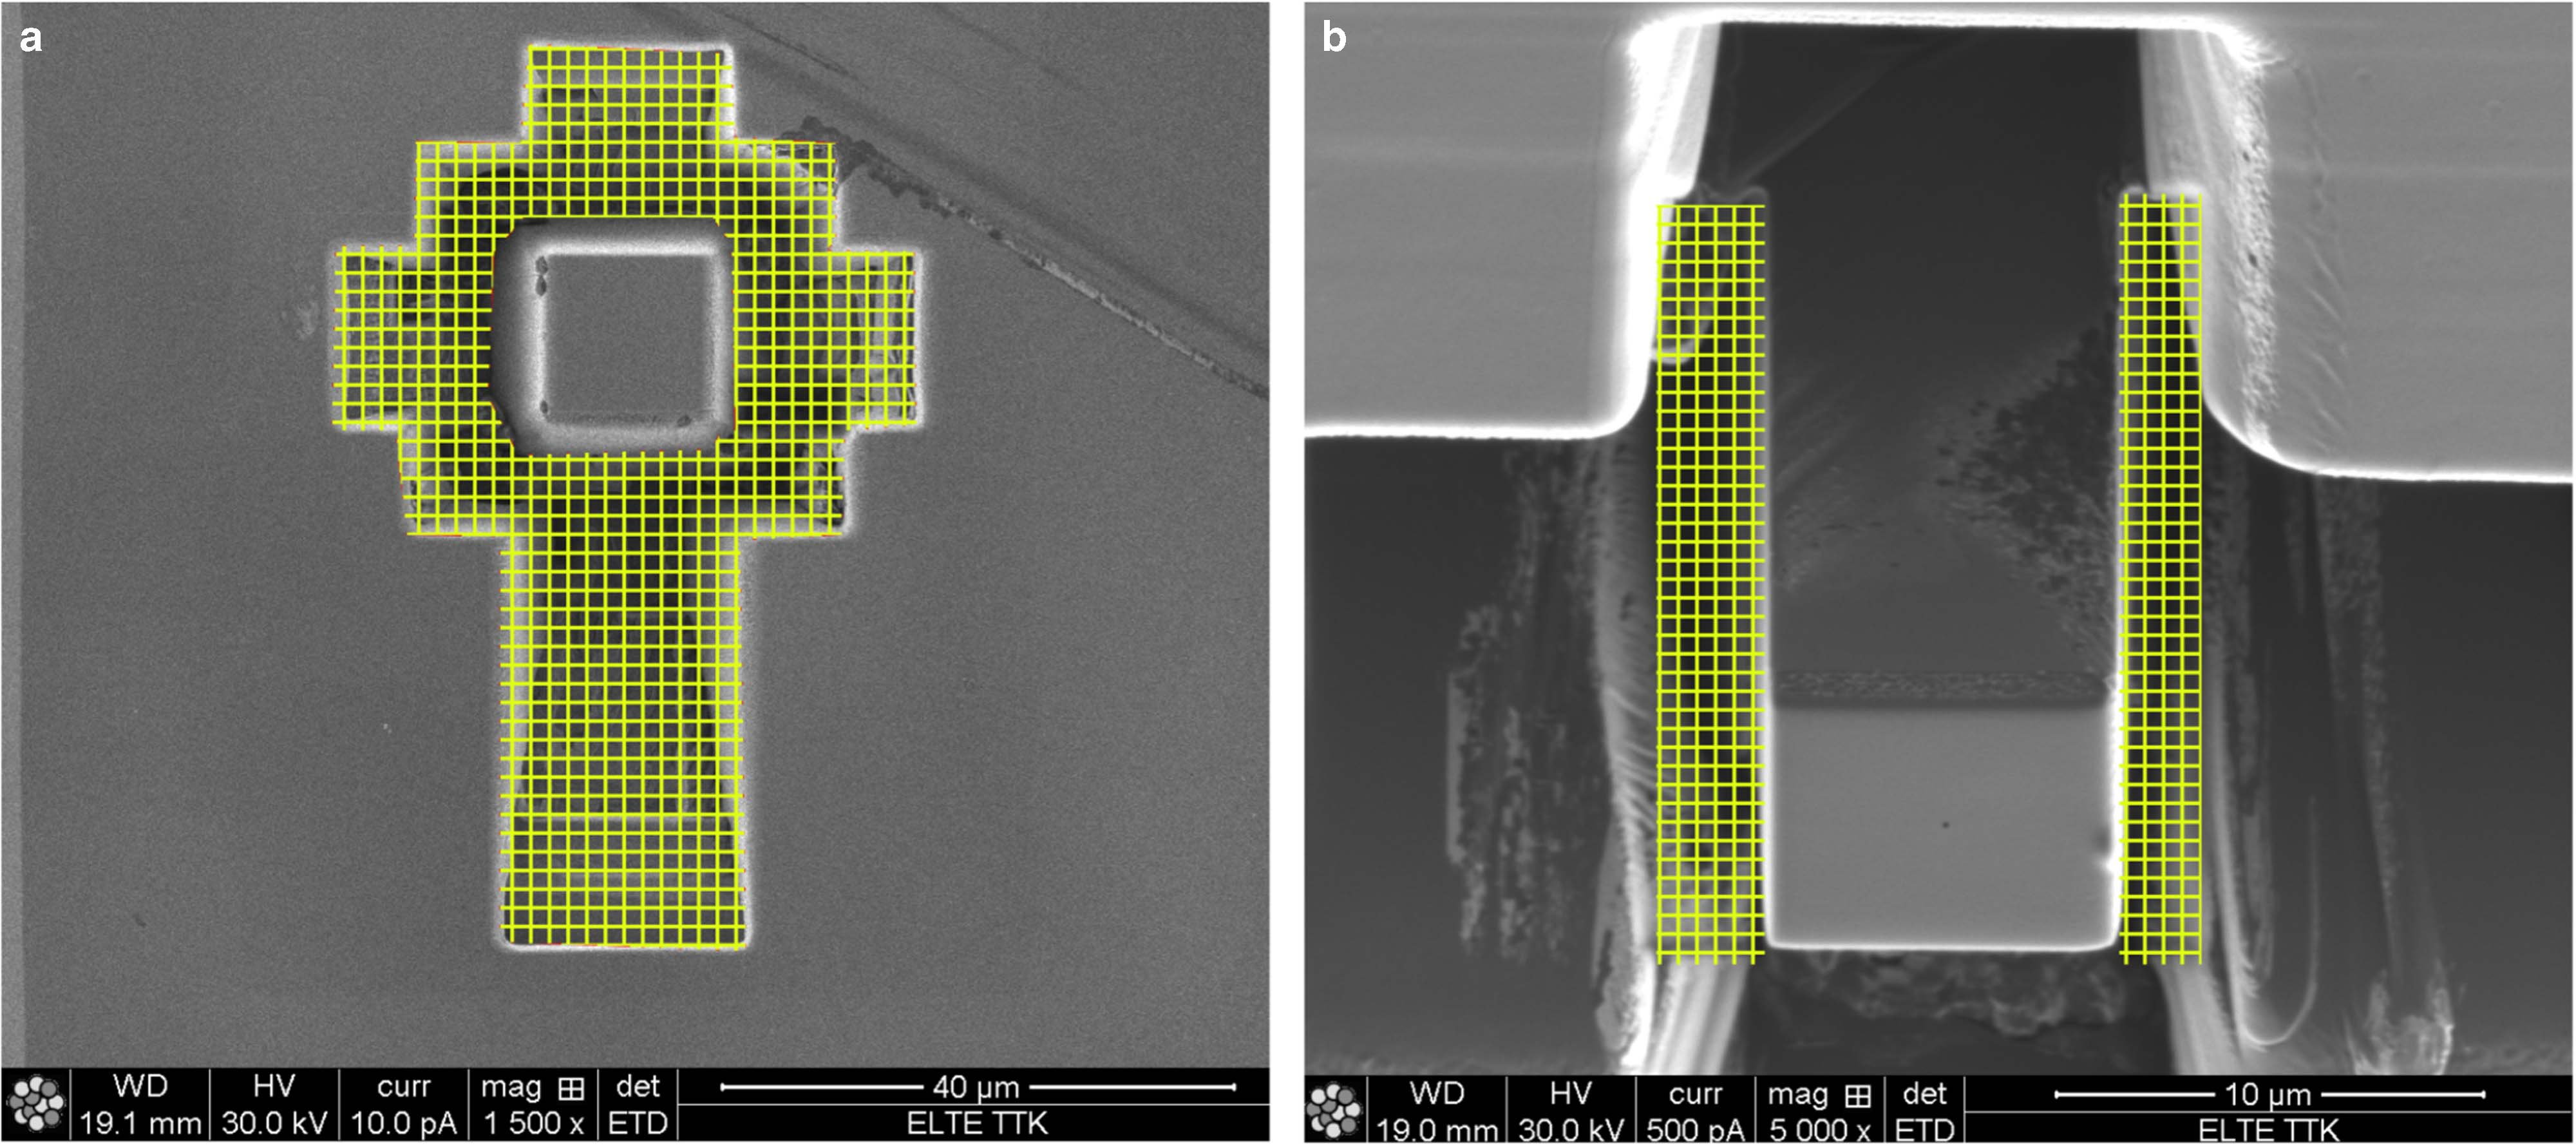
\includegraphics[width=1\textwidth]{Micron-Scale_Deformation2}
\caption[Raw and final pillar fabrication]{Both latheral and annular approaches were used during micropillar fabrication.\\
\textbf{(a)} The pillar was first hewed from the surface. FIB was directed from the point of view perpendicular to the surface marked by the yellow grid at \SI{30}{nA} current and at high voltage to create a whole around the pillar to fasten up further fabrication. The limb at the bottom provides a good view angle during the compression test. \\
\textbf{(b)} During the final milling step the sample was tilted by \SI{45}{\degree} and a smaller ion current of \SI{5}{nA} was used. The FIB was directed from the point of view to the yellow grid. In this step the top of the micropillar was already coated by a thin layer of Pt for protection.}
\label{fig:FIB_approaches}
\end{figure}

Apart from the rough digging mentioned in the first step, high milling angles were used in step~5. Despite the lower digging speed of the last milling steps the whole process was \numrange{2.5}{3} times faster then the commonly used perpendicular-only ion beam setup \cite{doi:10.1093/jmicro/dfh078}. The last step may also help to decrease the Ga ion implantation \cite{bei2007effects} even though it could be improved or revised \cite{greer2008comment}.

The following points sum up the most important features of the milling procedure proposed in this study.\begin{itemize}
\item Micropillars can be fabricated from any part of the flat surface of the bulk sample.
\item Micropillar preparation is touchless, thus damage or predeformation of the pillar can be arbitrary predefined or completely avoided during the the entire production procedure.
\item The final shape of the pillar is taper-free, i.e.\ the inclination of the side of the pillar was less than \SI{\pm0.5}{\degree}.
\item The method is considerably faster than the one suggested earlier, with a net mean milling time of less than \SI{4}{\hour} for the pillar size used in this study (\num{4 x 4 x 12}~\si{\micro m^3}).
\item FIB induced pillar hardening due to Ga implantation is decreased.
\end{itemize}

\begin{figure}[htbp!] 
\centering    
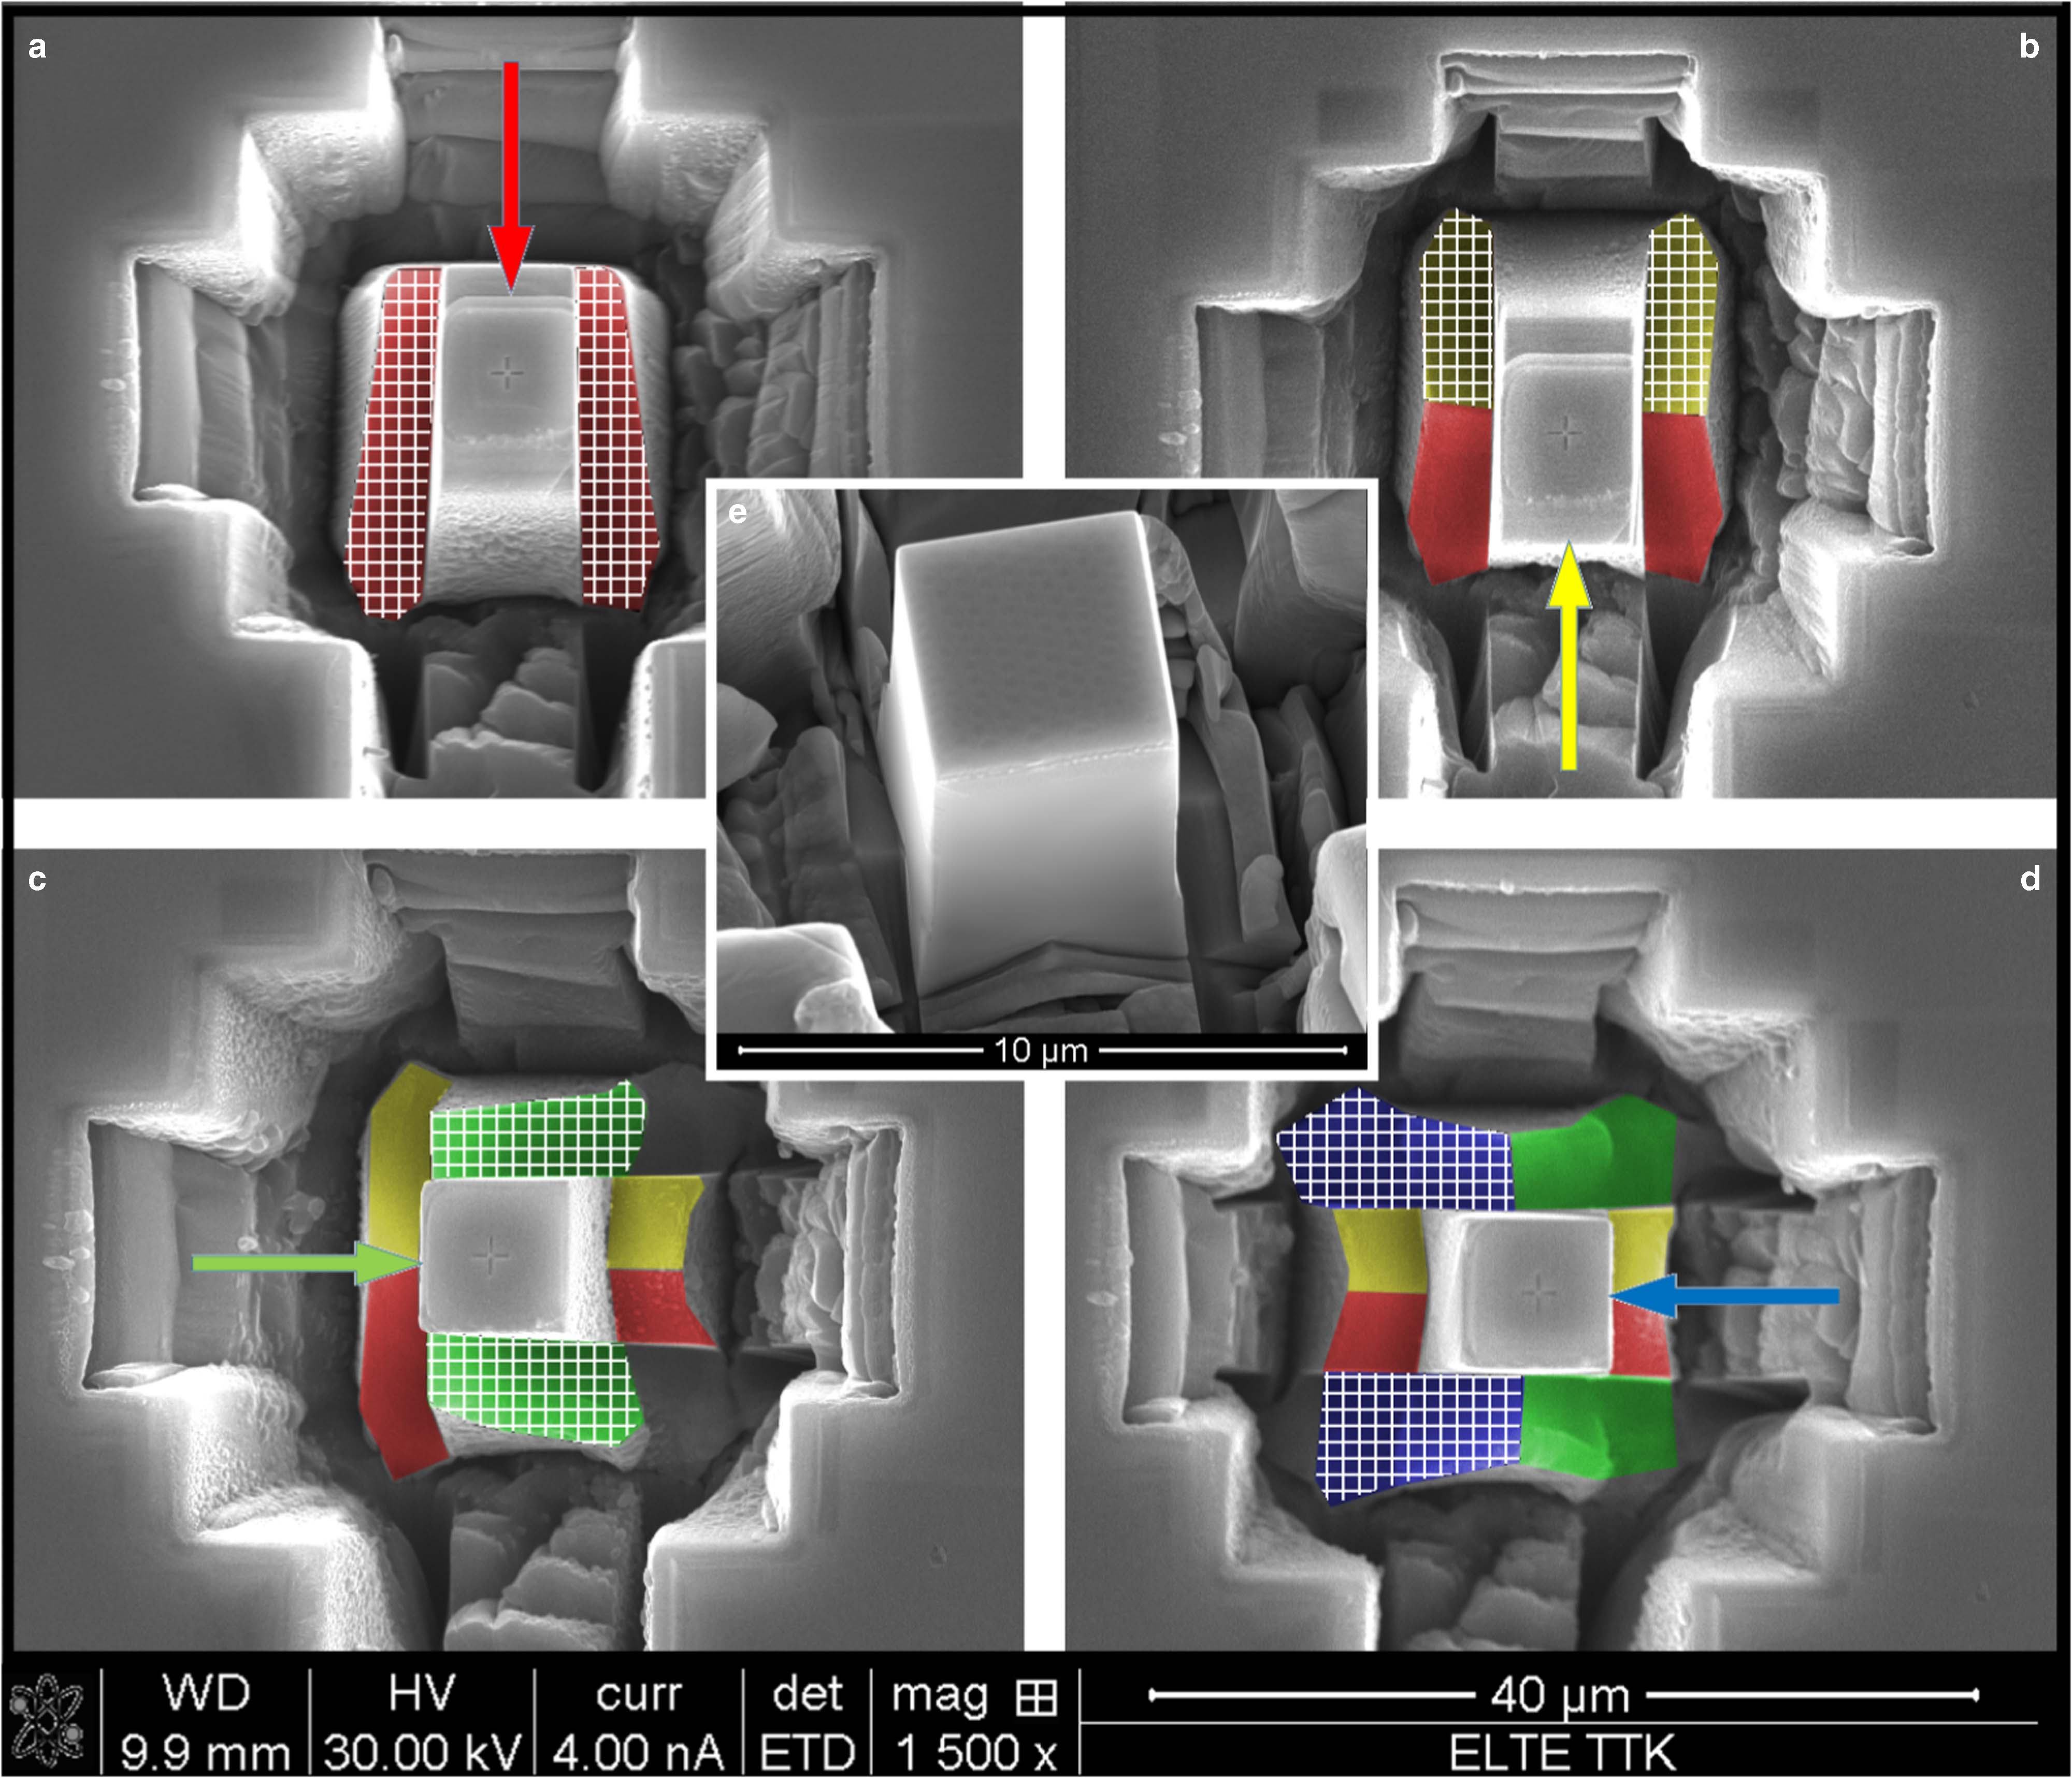
\includegraphics[width=1\textwidth]{Micron-Scale_Deformation}
\caption[Final pillar fabrication details]{Step~5 during pillar fabrication is detailed in this figure. Ion current was \SI{5}{nA}.\\
\textbf{(a)} Right after the raw pillar fabrication showed in Fig~\ref{fig:FIB_approaches}a. the sample was rotated around the pillar axis by a total of \SI{45}{\degree}. FIB was directed to two rectangular area merked by a red grid.\\
\textbf{(b)} The sample was rotated by \SI{180}{\degree} around the pillar axis. FIB was directed to the yellow grid to form the same sides of the sample but from the other direction.\\
\textbf{(c)} The sample was rotated by \SI{90}{\degree} around the pillar axis and the beam was directed to the green grid.\\
\textbf{(d)} The sample was rotated by \SI{180}{\degree} around the pillar axis to finish the shaping of the last two sides. FIB is directed onto the blue grid area.\\
\textbf{(e)} Steps \textbf{a-d} already gave a rectangular shaped pillar but to gain an even smoother shape they were repeated under \SI{1}{nA} first and \SI{0.1}{nA} second. The final pillar is shown in the inset.}
\label{fig:FIB_sides}
\end{figure}


\section{In situ device}
For an in situ micromechanical test the testing device has to fit into the vacuum chamber of the SEM. Such compression devices are commercially available, yet we used an inexpensive solution. The device easily fits into the vacuum chamber of a FEI Quanta 3D SEM\footnote{Produced by FEI, Hillsboro, Oregon, USA}. A schematic sketch is shown in Fig.~\ref{fig:nanotest_schematic}.

Two linear ultrasonic motors (denoted by X and Y in Fig.~\ref{fig:nanotest_schematic}) position the sample in the $x$ and $y$ directions. The AE detector is mounted on the top of the motors X and Y. In $z$ direction the sample can be moved by two motors. The first stage is moved by a gross linear step motor for raw movement moving the sample \SI{0.1}{mm} close to the indentation tip. The second stage is moved by a piezoelectric motor (piezoelectric positioning, PEP) with a resolution of \SI{0.1}{nm}. Only this stage is used for the compression test. The in-house fabricated spring -- which has a low longitudinal but high transversal stiffness -- is mounted onto the PEP stage and its movement is registered by the Z distance sensor, a capacitive sensor with a resolution of \SI{0.1}{nm}. With this latter two units both the deformation of the sample and the force can be determined. The deformation of the sample is $\epsilon = d-e$, where $d$ is the prescribed movement of the PEP stage (by Z fine) and $e$ is the measured elongation of the spring (by Z distance). The acting force can be calculated from $F=k \cdot e$, where $k$ is the spring constant determined from calibration. For pillar compression a flat punch diamond tip was used. To avoid static charges each item was grounded and a weakly conducting boron-doped tip was used.

To benefit from the high precision motors and sensors thermal and elastic elongation of the device must be prevented during the compression tests which take typically several minutes. To keep the temperature of the sample, X and Y motors constant, a Peltier cooling system was also mounted. The cold point of the cooling system was mounted onto the stage while the hot point was mounted onto the Quanta 3D SEM's appropriate, preconceived spot for Peltier cooling. This setup stabilised the temperature of the sample at \SI{15}{\celsius}. As the spring behaves as an harmonic oscillator one has to deal with this disturbing effect. In an in-air environment air flows between the lamellae providing the necessary damping, but this is not the case in a vacuum chamber. Strong permanent magnets were installed next to the spring body to generate eddy current in order to provide the necessary damping.



\begin{figure}[htbp!] 
  \centering
    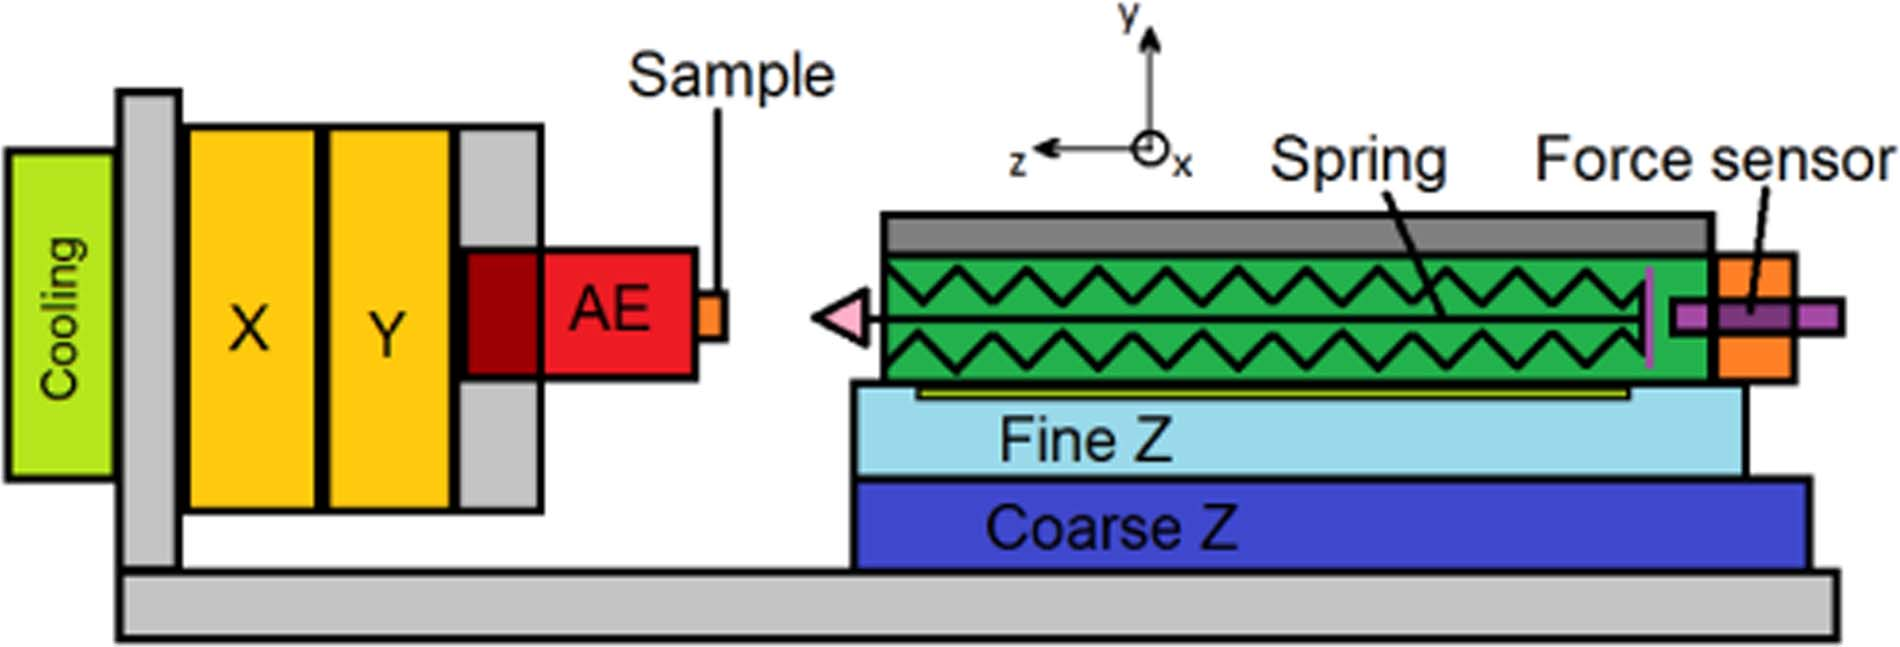
\includegraphics[width=0.5\textwidth]{nanotest}
    \caption{The X, Y, Z fine, Z gross and Z distance sensor are commercially available products while the frame, the cooling, and the Z force motor are in-house designed.\label{fig:nanotest_schematic}}
\end{figure}

To capture the phenomena caused by the PLC effect and dislocation avalanches, a minimum data collection rate of \SI{1}{k\hertz} is required along with a fast feedback controlling system, faster than any commercially available products. An analogous proportional-integral-derivative-type feedback electronics is developed in-house and used along with a fast 16 bit AD converter. The range and resolution parameters available for our device are summarised in table~\ref{table:nanotest_paramters}

\begin{table}[htbp]
\centering
\caption[NanoTest parameters]{The main parameters of our NanoTest device. The force sensor has two operating modes and can be improved or adjusted as the spring is interchangeable.}
\label{table:nanotest_paramters}
\begin{tabular}{llll}
\hline
\multicolumn{1}{c}{Part name} & \multicolumn{1}{c}{total range} & \multicolumn{1}{c}{resolution} & accuracy \\ \hline
X and Y stages  & \SI{\pm8}{mm}         & \SI{0.5}{\micro\meter} & \SI{0.01}{\micro\meter} \\
Z gross stage   & \SI{9}{mm}            & \SI{2}{\micro\meter}   & \SI{0.5}{\micro\meter}  \\
Z fine stage    & \SI{35}{\micro\meter} & \SI{1}{\nano\meter}    & \SI{0.1}{\nano\meter}   \\
Force sensor    & \SIlist{20;50}{mN}   & \SIlist{1;2.5}{\micro\newton} & \SIlist{1;2.5}{\micro\newton}   \\ \hline
\end{tabular}
\end{table}

\section{Acoustic emission measurements}
An AE measuring system was installed right below the sample to study the dynamic processes during the compression of the micropillars. An AE detector detects the transient elastic waves generated by fast elastic energy release processes. Such signals are originated from localised structural rearrangements, such as collective dislocation motion or twinning. As a consequence AE detectors can provide information on dynamic phenomena involved in plastic deformation \cite{heiple1987acoustic}.

AE signals can be used in bulk materials to identify the deformation mechanisms activated at different stages of the stress-strain curve \cite{BOHLEN2004214,PhysRevB.76.224110,dobrovn2009acoustic,KOVACS2014113}. The motion of a single dislocation creates vibration with a characteristic energy below the sensitivity of AE detectors. At least dozens or hundreds of dislocations must move at the same time to generate an "audible" signal for AE detectors meaning that AE signals correspond to collective dislocation motion \cite{doi:10.1179/msc.1981.15.11-12.599}. AE detection was already used in bulk samples, as the crackling or avalanche-like plastic response does not only characterise micron-scale objects \cite{PhysRevB.76.224110}, but due to the huge number of simultaneously moving dislocations in bulk materials, the contribution of each avalanche to the total strain is smaller and smaller as the specimen size increases which results in a smooth stress-strain curve at a specimen size of a millimetre. Therefore AE can be a valuable technique on the macro scale to provide information about the underlying mechanism that cannot be revealed from the stress-strain curves solely. To our knowledge, the first successful investigation of AE signals from micron-sized pillars was performed in the framework of this study.

A Physical Acoustics PCI-2 acquistion board was used to capture and store the preamplified AE signals from the detector until the readout. A \SI{60}{\decibel} gain was applied on the direct signal of the detector between the frequency range from \SIrange{100}{1200}{kHz} then the board mentioned sampled the signal at a \SI{2}{MHz} rate between \SI{\pm 10}{V} using a \SI{18}{bit} A/D converter. The noise of the card (without detector) is \SI{17}{\decibel} and with the detector attached to the surface inside the vacuum chamber was not larger than \SI{24}{\decibel}, which is in agreement with the product bulletin provided by the product manufacturer. In our experiment a threshold level \SI{26}{\decibel} was used. The signal was recorded simultaneously with the stress and strain data.

The series of micropillars were fabricated from the same grain. The sample was pressed against the AE transducer using a metallic spring. To improve the acoustic contact, vacuum grease was also used to fill up the gap between the AE transducer and the sample.

A constant strain rate was applied on the Al - 5\%Mg micropillar during the test. The calculated force and the AE signal recorded are plotted in Fig.~\ref{fig:loadAE_time}. As it can be seen in the figure the sample shows the well-known PLC instability. It is suspected that the stress drops correspond to the collective depinning of the dislocations from the solute atoms as obstacles generating a measurable AE signal marked by the four red lines. From  the negative slope of stress-real strain curve one can identify the strep-drops.

\begin{figure}[htbp!] 
\centering    
\includegraphics[width=0.6\textwidth]{Micron-Scale_Deformation3}
\caption[Load curve and AE signals]{The load and the local maximum of the AE signal versus time obtained from a micropillar compression test under constant strain rate are plotted.\\
\textbf{(a)} Inset \textit{a} shows a typical stress drop enlarged.\\
\textbf{(b)} Inset \textit{b} shows the waveform of an individual AE peak on a \si{m\second} scale.}
\label{fig:loadAE_time}
\end{figure}

Further investigations are required to unfold how stress drops caused by the PLC instability differ from the stress drops caused by dislocation avalanches. Such a comparison could be set up using non-PLC capable pure Al micropillars. As seen in Fig.~\ref{fig:loadAE_time}a, large AE signal is detected right before the onset of the stress drop. The PLC effect can suppress or at least compete with the intrinsic intermittent dislocation motion originated from dislocation avalanches, especially at size scale of the fabricated micropillar (\SI{4x4x12}{\micro m^3}). This two effects screen the well-known periodic stress drop structure of the stress-strain curve by introducing uncorrelated stress-drops due to dislocation avalanches.

The distinguishable large peaks in the acoustic signal shown in Fig.~\ref{fig:loadAE_time}b indicate that AS signal detection related to dislocation avalanches may be feasible even for samples with a small volume of \SI{100}{\micro m^3}.

\section{Summary}
The plastic response caused by the external stress shows intermittent characteristic at the micron scale, a phenomenon not observed in bulk samples. Although the stress-strain curve from compression test differs in general from sample to sample but they may share similar behaviour and an approach based on statistical investigation can be suitable to unravel the underlying stochastic processes and identify some parameter characterising the system examined. Therefore numerous tests must be performed requiring micropillars are needed. For that reason the efficiency of the technique used for micropillar fabrication must be improved in order to produce micropillars in a number suitable for statistical ensembling.

A high precision, fast-feedback micromechanical compression device was used in our laboratory to measure the stress and strain during the compression with extra care. All the data and the in situ SEM arrangement validate the plausible assumptions based on AE signal detection. The unit of the three mutually supportive investigation method gives an original tool suitable to perform micromechanical tests at the aim of revealing the stochastic properties of micron scale plasticity.

\section*{Notes in regard to the thesis}
In this study technological advancement in micropillar fabrication and compression were introduced. It is well emphasised how important they are in order to start mass investigation on micron scale plasticity and a demonstrative example was also given. At this stage one cannot compare yet the properties of micron scale plasticity obtained theoretically with the ones observed experimentally in this study, but the step made here is elementary necessary to achieve this goal. Ongoing research with new results are already available but not achieved the state of a publishable level.

My specific contribution to this study is the following. I played a role in the selection and pretreatment of the cast aluminum and I was also involved in the dislocation density measurement performed by X-ray line profile analysis. Even though many times it required abilities not associated with the skills of a doctoral student in physics, these engineering-like challenges must have been solved to take a step further in the field of micron scale plasticity.

I look forward for challenges in the improvement of the force sensor, the AE signal detection and the data analysis. I believe the resource requested is given to fabricate numerous PLC and non-PLC micropillars, the compression test would serve valuable information on their behaviour and a comparison with bulk samples could provide the next step further for characterising micron scale plasticity.


%!TEX root = ../thesis.tex
%*******************************************************************************
%****************************** Seventh Chapter **********************************
%*******************************************************************************
\chapter[Summary, összefoglaló]{Summary, összefoglaló} \label{chapter:summary}
\section*{In English}
The topic of my doctoral thesis was inspired by the diversity of the collective and stochastic properties of dislocations. Nowadays the size scales accessible for computational simulations and experiments overlap for crystalline materials. They can be modelled with computers and can be investigated by, for example, scanning electron microscopes, even in an in-situ deformation setup too.

As the first step of my thesis I approached the issue from a theoretical point of view. I developed a cellular automaton model based on the continuum theory of dislocations and investigated the role of the relevant parameters in the region of small deformations. The model handles the flow stress on cell-level ($\tau_w$) and it is considered as a random variable and calibrated via lower scale, discrete dislocation dynamic (DDD) simulations. The expected value of $\tau_w$ and the size of the applied discrete plastic strain on the cells are calibrated via the comparison of the stress-strain curve of the CA model and two other DDD models. The efficiency of the multiscale modelling is reflected on that that beyond the fitted properties of the model it shows the same type of universality classes with the DDD simulations. Based on the findings a plasticity model has been also introduced.

The CA model is applicable on materials with internal disorder that undergo strain softening, if the fracture is due to strain localisation. To model this behaviour a softening mechanism has been introduced. The disorder in the material is provided by the distribution of $\tau_w$. The results of the simulations show, that in materials with higher disorder the applicable highest stress is significantly larger, and failure occurs at considerably larger plastic strain.

The CA models used above has strong assumptions on dislocation correlations. To this end the equation of motions of the CA model is extended with stress terms attributable to these correlations. Linear stability analysis (LSA) shows the possibility of dislocation pattern formation and link the free parameters of the model to the characteristic wavelength of the pattern. My simulation results obtained from this CA model follows well the prediction of the LSA, so does a non-discrete model, where in contrary to the extremal dynamics of the CA, hydrodynamic-like transport equations are used. Despite the elemental differences between the models they both built upon new stress terms attributed to the more precise continuum theory, and therefore they indeed show qualitatively same results, showing the robustness of the theory.

In the last part of my thesis I approached the topic from an experimental point of view. In the micron scale the plastic deformation of crystalline materials show avalanche-like behaviour. The key of the research work is the recognition, that in this size scale the deformation response of each micron-sized sample is different from sample to sample, therefore, characterisation of materials must rely on a statistical approach. This requires a large amount of data measured on the samples, and the origin of the data measured must be well interpreted and evaluated. To this and, at one hand, a new micropillar-fabrication method is proposed facilitating the mass production of the samples with the required shape. On the other hand, a unique experimental setup has been implemented making it possible to track the in-situ compression procedure faster than ever before in an electron microscope, and due to an attached acoustic emission detector coupling the avalanches observed with the acoustic signals detected became possible.

\section*{Magyarul}
Doktori tézisem témáját a diszlokációk mozgásának kollektív és sztochasztikus tulajdonságainak a sokszínűsége biztosította. Ma már a vizsgált kristályos anyagok méretskálái összeérnek a numerikus szimulációs és a kísérleti oldalról: olyan anyagok modellezhetőek számítógéppel, amelyek vizsgálhatóak pl. pásztázó elektronmikroszkópban, akár in-situ deformáció közben is.

Doktori munkám első lépéseként elméleti úton közelítettem meg a témakört. A diszlokációk kontinuum-elméleti leírására épülő sejtautomata (CA) modellt fejlesztettem és vizsgáltam a releváns paraméterek szerepét a kis deformációk tartományában. A CA modellben a cellaszintű folyáshatárt ($\tau_w$-t) véletlen változóként kezeltem, és alacsonyabb skálájú, diszkrét diszlokációdinamikai modellek alapján kalibráltam. A $\tau_w$ várható értékét és a cellákban alkalmazott diszkrét deformációs lépés nagyságát pedig a CA, és két másik DDD modell feszültség-deformációs görbéi alapján kalibráltam. A CA modell eredményessége abban mutatkozik meg, hogy az illesztett tulajdonságokon felül a modell azonos típusú univerzális skálázási tulajdonságokat mutat, mint a DDD szimulációk. Az eredmények alapján egy plaszticitás modell is bemutatásra került.

A CA modell alkalmazható olyan alakítási lágyulást szenvedő anyagok törésének modellezésére is, ahol a törést a deformáció lokalizáció okozza. Ehhez bevezettem a modellben egy lágyulási mechanizmust. Az így kapott modellben a rendszer rendezetlenségét a $\tau_w$ eloszlása biztosítja. A szimulációk eredménye azt mutatta, hogy a nagyobb rendezetlenségű anyagokban az alkalmazható maximális feszültség jelentősen nő és jóval nagyobb plasztikus deformáció után következik be a törés.

A fentebb használt CA modell erős feltételezéseket tesz a diszlokáció korrelációkra. Ezért a CA modell mozgásegyenleteit kiegészítettem olyan továbbá feszültségtagokkal, amelyek eredete a korrelációkra vezethető vissza. Lineáris stabilitásanalízis (LSA) alapján tudható, hogy lehetőség van diszlokációmintázatok fejlődésére, valamint az LSA kapcsolatot teremt a modell szabad paraméterei és a mintázat jellemző hullámhossza között. A CA szimulációs eredményei azt mutatták, hogy a modell jól követi az LSA jóslatát, hasonlóan egy nem diszkrét, és a CA modell extrém dinamikájával szemben egy hidrodinamika-szerű transzport-egyenletet használó modellel. Ez a kétfajta megvalósítás alapvetően különbözik egymástól, de ugyanazokon, a pontosabb kontinuumelmélethez tartozó új erőkön alapulnak, és eredményeink alapján éppen ezért minőségileg azonos eredményt is adnak, amely mutatja az elmélet robusztusságát.

A doktori munkámat a téma kísérleti oldalról való megközelítésével zártam. Itt a mikron méretű fémes anyagok plasztikus deformációjában megjelenő lavinaszerű viselkedés vizsgálata volt az előtérben. A munka kulcseleme, hogy ezen a méretskálán minden egyes mikroméretű kristály deformációs válasza más és más, így az anyagoknak csak statisztikai értelemben adhatunk tulajdonságokat. Ehhez elengedhetetlen, hogy nagymennyiségű adatot lehessen a mintákról összegyűjteni, és hogy a mért adatok fizikai háttere világos legyen. Ennek elősegítése céljából egyrészt egy új mikrooszlop-megmunkálási eljárást javasoltunk, amellyel minden eddiginél gyorsabban lehet a kívánt alakú mikrooszlopokat előállítani. Másrészt egy unikális kísérleti összeállítást valósítottunk meg, amelynek segítségével minden eddiginél gyorsabb lekövetéssel lehetséges a mikrooszlopok összenyomásának in-situ elektronmikroszkópos vizsgálata, így egy csatolt akusztikus emissziós detektorral pontosan párosítani tudjuk a diszlokáció lavinákat és az érzékelt akusztikus jeleket.

%!TEX root = ../thesis.tex
%*******************************************************************************
%****************************** Seventh Chapter **********************************
%*******************************************************************************
\chapter{Own publications related to the thesis} \label{chapter:publications}

% **************************** Define Graphics Path **************************
\ifpdf
    \graphicspath{{Chapter7/Figs/Raster/}{Chapter7/Figs/PDF/}{Chapter7/Figs/}}
\else
    \graphicspath{{Chapter7/Figs/Vector/}{Chapter7/Figs/}}
\fi

\begin{itemize}
\item [{[O1]}]

\begin{description}
\item [Title:] Role of weakest links and system-size scaling in multiscale modeling of stochastic plasticity
\item [Publisher:] American Physical Society
\item [Journal:] \href{https://doi.org/10.1103/PhysRevB.95.054108}{Physical Review B, Volume 95, Issue 5, Pages 054108, Year 2017}
\item [Authors:] Péter Dusán Ispánovity$^*$, Dániel Tüzes$^{* \dagger}$, Péter Szabó$^*$, Michael Zaiser$^\dagger$, and István Groma$^*$
\item [Institutes:]~
\begin{description}
\item [$^*$] Eötvös Loránd University, Department of Materials Physics, 1117, Pázmány Péter sétány 1/a., Budapest, Hungary
\item [$^\dagger$] Friedrich-Alexander University Erlangen-Nürnberg (FAU), Institute for Materials Simulation, Department of Materials Science, 90762, Dr.-Mack-Straße 77, Fürth, Germany
\end{description}
\end{description}\label{paper:A2}

\pagebreak

\item [{[O2]}] \label{paper:A3}
\begin{description}
\item [Title:] Disorder is good for you: the influence of local disorder on strain localization and ductility of strain softening materials
\item [Publisher:] Springer Netherlands
\item [Journal:] \href{https://doi.org/10.1007/s10704-017-0187-1}{International Journal of Fracture, Volume 205, Issue 2, Pages 139–150}
\item [Authors:] Dániel Tüzes$^{* \dagger}$, Péter Dusán Ispánovity$^*$, and Michael Zaiser$^\dagger$
\item [Institutes:]~
\begin{description}
\item [$^*$] Eötvös Loránd University, Department of Materials Physics, 1117, Pázmány Péter sétány 1/a., Budapest, Hungary
\item [$^\dagger$] Friedrich-Alexander University Erlangen-Nürnberg (FAU), Institute for Materials Simulation, Department of Materials Science, 90762, Dr.-Mack-Straße 77, Fürth, Germany
\end{description}
\end{description}
\noindent\rule{8cm}{0.4pt}


\item [{[O3]}] \label{paper:A4}
\begin{description}
\item [Title:] Instability of dislocation fluxes in a single slip: Deterministic and stochastic models of dislocation patterning
\item [Publisher:] American Physical Society
\item [Journal:] \href{https://doi.org/10.1103/PhysRevB.98.054110}{Physical Review B, Volume 98, Issue 5, Pages 054110, Year 2018}
\item [Authors:] Ronghai Wu$^{\dagger \ddagger}$, Daniel Tüzes$^*$, Péter Dusán Ispánovity$^*$, István Groma$^*$, Thomas Hochrainer$^\mathsection$, and Michael Zaiser$^{\dagger \mathparagraph}$
\item [Institutes:]~
\begin{description}
\item [$^\dagger$] Friedrich-Alexander University Erlangen-Nürnberg (FAU), Institute for Materials Simulation, Department of Materials Science, 90762, Dr.-Mack-Straße 77, Fürth, Germany
\item [$^\ddagger$] School of Mechanics, Civil Engineering, and Architecture, Northwestern Polytechnical University, Xian, 710129, People’s Republic of China
\item [$^*$] Eötvös Loránd University, Department of Materials Physics, 1117, Pázmány Péter sétány 1/a., Budapest, Hungary
\item [$^\mathsection$] Institut für Festigkeitslehre, Technische Universität Graz, Kopernikusgasse 24/I, 8010 Graz, Austria
\item [$^\mathparagraph$] Department of Mechanics and Engineering, Southwest Jiaotong University, Chengdu, People’s Republic of China
\end{description}
\end{description}

\pagebreak

\item [{[O4]}] \label{paper:A1}
\begin{description}
\item [Title:] Micron-Scale Deformation: A Coupled In Situ Study of Strain Bursts and Acoustic Emission
\item [Publisher:] Cambridge University Press
\item [Journal:] \href{https://doi.org/10.1017/S1431927617012594}{Microscopy and Microanalysis, Volume 23, Number 6, Pages 1076--1081, Year 2017}
\item [Authors:] Hegyi Ádám$^*$, Péter Dusán Ispánovity$^*$, Michal Knapek$^\|$, Dániel Tüzes$^*$, Kristián Máthis$^\|$, František Chmelík$^\|$, Zoltán Dankházi$^*$, Gábor Varga$^*$, and István Groma$^*$
\item [Institutes:]~
\begin{description}
\item [$^*$] Eötvös Loránd University, Department of Materials Physics, 1117, Pázmány Péter sétány 1/a., Budapest, Hungary
\item [$^\|$] Faculty of Mathematics and Physics, Department of Physics of Materials, Charles University in Prague, Ke Karlovu 5, 121 16 Prague 2, Czech Republic
\end{description}
\end{description}
\end{itemize}







% ********************************** Back Matter *******************************
% Backmatter should be commented out, if you are using appendices after References
%\backmatter

% ********************************** Bibliography ******************************
\begin{spacing}{0.9}

% To use the conventional natbib style referencing
% Bibliography style previews: http://nodonn.tipido.net/bibstyle.php
% Reference styles: http://sites.stat.psu.edu/~surajit/present/bib.htm

%\bibliographystyle{apalike}
%\bibliographystyle{unsrt} % Use for unsorted references  


\bibliographystyle{plainnat} % use this to have URLs listed in References
\cleardoublepage
\bibliography{References/references} % Path to your References.bib file

%\bibliographystyleown{plainnat} % use this to have URLs listed in References
%\cleardoublepage
%\bibliographyown{References/references2} % Path to your References.bib file

% If you would like to use BibLaTeX for your references, pass `custombib' as
% an option in the document class. The location of 'reference.bib' should be
% specified in the preamble.tex file in the custombib section.
% Comment out the lines related to natbib above and uncomment the following line.

%\printbibliography[heading=bibintoc, title={References}]


\end{spacing}

% ********************************** Appendices ********************************

\begin{appendices} % Using appendices environment for more functunality

%!TEX root = ../thesis.tex
% ******************************* Thesis Appendix A ****************************
\chapter{Dimensionless units}\label{sec:dimensionless_units}
In the case when dislocation cores can be considered pointlike (e.g.\ all the size scales are orders of magnitude larger), dislocation systems are invariant under the following scaling transformation:
\begin{align}
  {\mathbf{r}} \mapsto {\mathbf{r}}/c \hfill \\
  \gamma  \mapsto c \cdot \gamma  \hfill \\
  \tau  \mapsto c \cdot \tau,  \hfill \\ 
\end{align}
where $\mathbf{r}$ is the spatial coordinate, $\gamma$ is the plastic shear strain, and $\tau$ is the shear stress ($c>0$). This universal feature is a consequence of the $1/r$ type (scale-free) decay of the stress field of the dislocation. This also means that in an infinite dislocation system only one length scale can appear besides the size of the Burgers vector $b$, the mean dislocation distance $\rho^{-1/2}$, where $\rho$ is the average total dislocation density. We, therefore, introduce a dimensionless unit system by choosing $c=\rho^{-1/2}$ and divide all the quantities mentioned before with their corresponding natural material specific unit, 
\begin{alignat}{2}
  {\mathbf{r}}' =  & {\mathbf{r}}/{\rho ^{ - 1/2}} &&  = {\mathbf{r}}/{\rho ^{ - 1/2}} \\ 
  \gamma ' =  & {\rho ^{ - 1/2}}\gamma /b &&  = \gamma /\left( {b{\rho ^{1/2}}} \right) \\ 
  \tau ' =  & {\rho ^{ - 1/2}} \cdot \tau /\left( {\frac{{\mu b}}{{2\pi \left( {1 - \nu } \right)}}} \right) & & = \tau / \left( {\frac{{\mu b{\rho ^{1/2}}}}{{2\pi \left( {1 - \nu } \right)}}} \right), 
\end{alignat}
where $\mu$ is the shear modulus, $\nu$ is the Poisson ratio. At many parts of this thesis, these dimensionless units are used. This interesting and useful principle is elaborated in the work of \citet{0965-0393-22-6-065012}.
% %!TEX root = ../thesis.tex
% ******************************* Thesis Appendix B ********************************

\chapter{Installing the CUED class file}

\LaTeX.cls files can be accessed system-wide when they are placed in the
<texmf>/tex/latex directory, where <texmf> is the root directory of the user’s \TeX installation. On systems that have a local texmf tree (<texmflocal>), which
may be named ``texmf-local'' or ``localtexmf'', it may be advisable to install packages in <texmflocal>, rather than <texmf> as the contents of the former, unlike that of the latter, are preserved after the \LaTeX system is reinstalled and/or upgraded.

It is recommended that the user create a subdirectory <texmf>/tex/latex/CUED for all CUED related \LaTeX class and package files. On some \LaTeX systems, the directory look-up tables will need to be refreshed after making additions or deletions to the system files. For \TeX Live systems this is accomplished via executing ``texhash'' as root. MIK\TeX users can run ``initexmf -u'' to accomplish the same thing.

Users not willing or able to install the files system-wide can install them in their personal directories, but will then have to provide the path (full or relative) in addition to the filename when referring to them in \LaTeX.



\end{appendices}

% *************************************** Index ********************************
\printthesisindex % If index is present

\end{document}
